% Options for packages loaded elsewhere
\PassOptionsToPackage{unicode}{hyperref}
\PassOptionsToPackage{hyphens}{url}
%
\documentclass[
]{book}
\usepackage{lmodern}
\usepackage{amsmath}
\usepackage{ifxetex,ifluatex}
\ifnum 0\ifxetex 1\fi\ifluatex 1\fi=0 % if pdftex
  \usepackage[T1]{fontenc}
  \usepackage[utf8]{inputenc}
  \usepackage{textcomp} % provide euro and other symbols
  \usepackage{amssymb}
\else % if luatex or xetex
  \usepackage{unicode-math}
  \defaultfontfeatures{Scale=MatchLowercase}
  \defaultfontfeatures[\rmfamily]{Ligatures=TeX,Scale=1}
\fi
% Use upquote if available, for straight quotes in verbatim environments
\IfFileExists{upquote.sty}{\usepackage{upquote}}{}
\IfFileExists{microtype.sty}{% use microtype if available
  \usepackage[]{microtype}
  \UseMicrotypeSet[protrusion]{basicmath} % disable protrusion for tt fonts
}{}
\makeatletter
\@ifundefined{KOMAClassName}{% if non-KOMA class
  \IfFileExists{parskip.sty}{%
    \usepackage{parskip}
  }{% else
    \setlength{\parindent}{0pt}
    \setlength{\parskip}{6pt plus 2pt minus 1pt}}
}{% if KOMA class
  \KOMAoptions{parskip=half}}
\makeatother
\usepackage{xcolor}
\IfFileExists{xurl.sty}{\usepackage{xurl}}{} % add URL line breaks if available
\IfFileExists{bookmark.sty}{\usepackage{bookmark}}{\usepackage{hyperref}}
\hypersetup{
  pdftitle={Explore Military Design \& Innovation},
  pdfauthor={C.P. Corvers},
  hidelinks,
  pdfcreator={LaTeX via pandoc}}
\urlstyle{same} % disable monospaced font for URLs
\usepackage{longtable,booktabs}
\usepackage{calc} % for calculating minipage widths
% Correct order of tables after \paragraph or \subparagraph
\usepackage{etoolbox}
\makeatletter
\patchcmd\longtable{\par}{\if@noskipsec\mbox{}\fi\par}{}{}
\makeatother
% Allow footnotes in longtable head/foot
\IfFileExists{footnotehyper.sty}{\usepackage{footnotehyper}}{\usepackage{footnote}}
\makesavenoteenv{longtable}
\usepackage{graphicx}
\makeatletter
\def\maxwidth{\ifdim\Gin@nat@width>\linewidth\linewidth\else\Gin@nat@width\fi}
\def\maxheight{\ifdim\Gin@nat@height>\textheight\textheight\else\Gin@nat@height\fi}
\makeatother
% Scale images if necessary, so that they will not overflow the page
% margins by default, and it is still possible to overwrite the defaults
% using explicit options in \includegraphics[width, height, ...]{}
\setkeys{Gin}{width=\maxwidth,height=\maxheight,keepaspectratio}
% Set default figure placement to htbp
\makeatletter
\def\fps@figure{htbp}
\makeatother
\setlength{\emergencystretch}{3em} % prevent overfull lines
\providecommand{\tightlist}{%
  \setlength{\itemsep}{0pt}\setlength{\parskip}{0pt}}
\setcounter{secnumdepth}{5}
\usepackage{booktabs}
\ifluatex
  \usepackage{selnolig}  % disable illegal ligatures
\fi
\newlength{\cslhangindent}
\setlength{\cslhangindent}{1.5em}
\newlength{\csllabelwidth}
\setlength{\csllabelwidth}{3em}
\newenvironment{CSLReferences}[2] % #1 hanging-ident, #2 entry spacing
 {% don't indent paragraphs
  \setlength{\parindent}{0pt}
  % turn on hanging indent if param 1 is 1
  \ifodd #1 \everypar{\setlength{\hangindent}{\cslhangindent}}\ignorespaces\fi
  % set entry spacing
  \ifnum #2 > 0
  \setlength{\parskip}{#2\baselineskip}
  \fi
 }%
 {}
\usepackage{calc}
\newcommand{\CSLBlock}[1]{#1\hfill\break}
\newcommand{\CSLLeftMargin}[1]{\parbox[t]{\csllabelwidth}{#1}}
\newcommand{\CSLRightInline}[1]{\parbox[t]{\linewidth - \csllabelwidth}{#1}\break}
\newcommand{\CSLIndent}[1]{\hspace{\cslhangindent}#1}

\title{Explore Military Design \& Innovation}
\author{C.P. Corvers}
\date{2021-04-07}

\begin{document}
\maketitle

{
\setcounter{tocdepth}{1}
\tableofcontents
}
\hypertarget{voorwoord}{%
\chapter*{Voorwoord}\label{voorwoord}}
\addcontentsline{toc}{chapter}{Voorwoord}

Sinds januari 2019 heeft het Commando Landstrijdkrachten (CLAS) een vierde directie in de staf opgenomen, de directie Kennis \& Ontwikkeling (DK\&O). Onder deze directie worden drie afdelingen functioneel georganiseerd. Dit zijn de afdeling Strategie \& Plannen (S\&P), afdeling Regie (LWC/Regie) en de afdeling Innovatie (io). Deze laatste is een samenvoeging van de programma's De Adaptieve Krijgsmacht - CLAS (DAK-C) en Concept Development \& Experimentation (CD\&E). Deze organisatorische verandering is een volgende stap in het moderniseren en innoveren van de Landmacht en het landoptreden.

Innoveren in een complexe omgeving en aanpakken van ingewikkelde en ongetemde problemen is een ontdekkingstocht op onbekend terrein met een gevarieerd reisgezelschap. Dit digitale boek deelt ervaringen van eerdere reizigers en geeft tools en technieken die nuttig zijn tijdens de reis. Het beschrijft de ontwikkeling van een nieuw vak, hoe te denken en praktiseren als vakmens en waarom vakmensschap belangrijk is. In de opzet worden de Golden circles van Simon Sinek gevolgd door het redeneren vanuit het `why,' `how' en `what.' Waarom we de doelen willen nastreven (ambitie/effecten), hoe we bij ons doel kunnen komen (routes/activiteiten) en wat we nodig hebben om bij het doel te komen (capaciteiten/mensen/manieren/middelen).

Dit boek is geschreven met twee soorten lezers in gedachten. De vakmensen die zich wil inzetten voor modernisering van het landoptreden en de design-researchers die onderzoeken hoe de Koninklijke Landmacht transformeert richting de toekomst.

In de doorontwikkeling van de tools en technieken waren veel personen betrokken. Zij maakte allen onlosmakkelijk deel uit van het reisgezelschap. Sommige trokken een andere richting op, andere zijn ons vooruitgesneld. We herinneren met liefde en plezier alle reisgenoten en zijn dankbaar voor de leermomenten die we samen mochten ervaren.

\hypertarget{leeswijzer}{%
\subsubsection*{leeswijzer}\label{leeswijzer}}
\addcontentsline{toc}{subsubsection}{leeswijzer}

In chronologische volgorde komen de volgende onderwerpen voorbij.

\textbf{\protect\hyperlink{cde-algemeen}{Organisatie}}
geeft achtergrond kennis over de missie, conceptuele en organisatorische positionering en organisatiestructuur.

\textbf{\protect\hyperlink{kort-cyclisch-moderniseren}{How to think}}
beschrijft hoe te denken in effecten en effectbrengers.

\textbf{\protect\hyperlink{cde-design-model}{How to act}}
geeft handvatten in het ontwikkelen en experimenteren met effectbrengers zoals technieken en tools voor het articuleren, organiseren, uitvoeren en rapporteren. Ook beschrijft dit hoofdstuk hoe de effectbrengers in een samenwerking met interne- en externe partijen ontwikkeld wordt.

\textbf{\protect\hyperlink{cde-routines}{CD\&E routines}}
beschrijft procedures voor besluitvorming over moderniseringsvoorstellen.

\textbf{\protect\hyperlink{cde-process}{Ontstaansgeschiedenis en doorontwikkeling.}}
Transformatie is continue leren en vernieuwen, ook onze tools en technieken transformeren. In dit hoofdstuk zijn de eerdere versies van onze tools, technieken en structuren terug te lezen.

\hypertarget{intro}{%
\chapter{Introduction}\label{intro}}

\begin{figure}
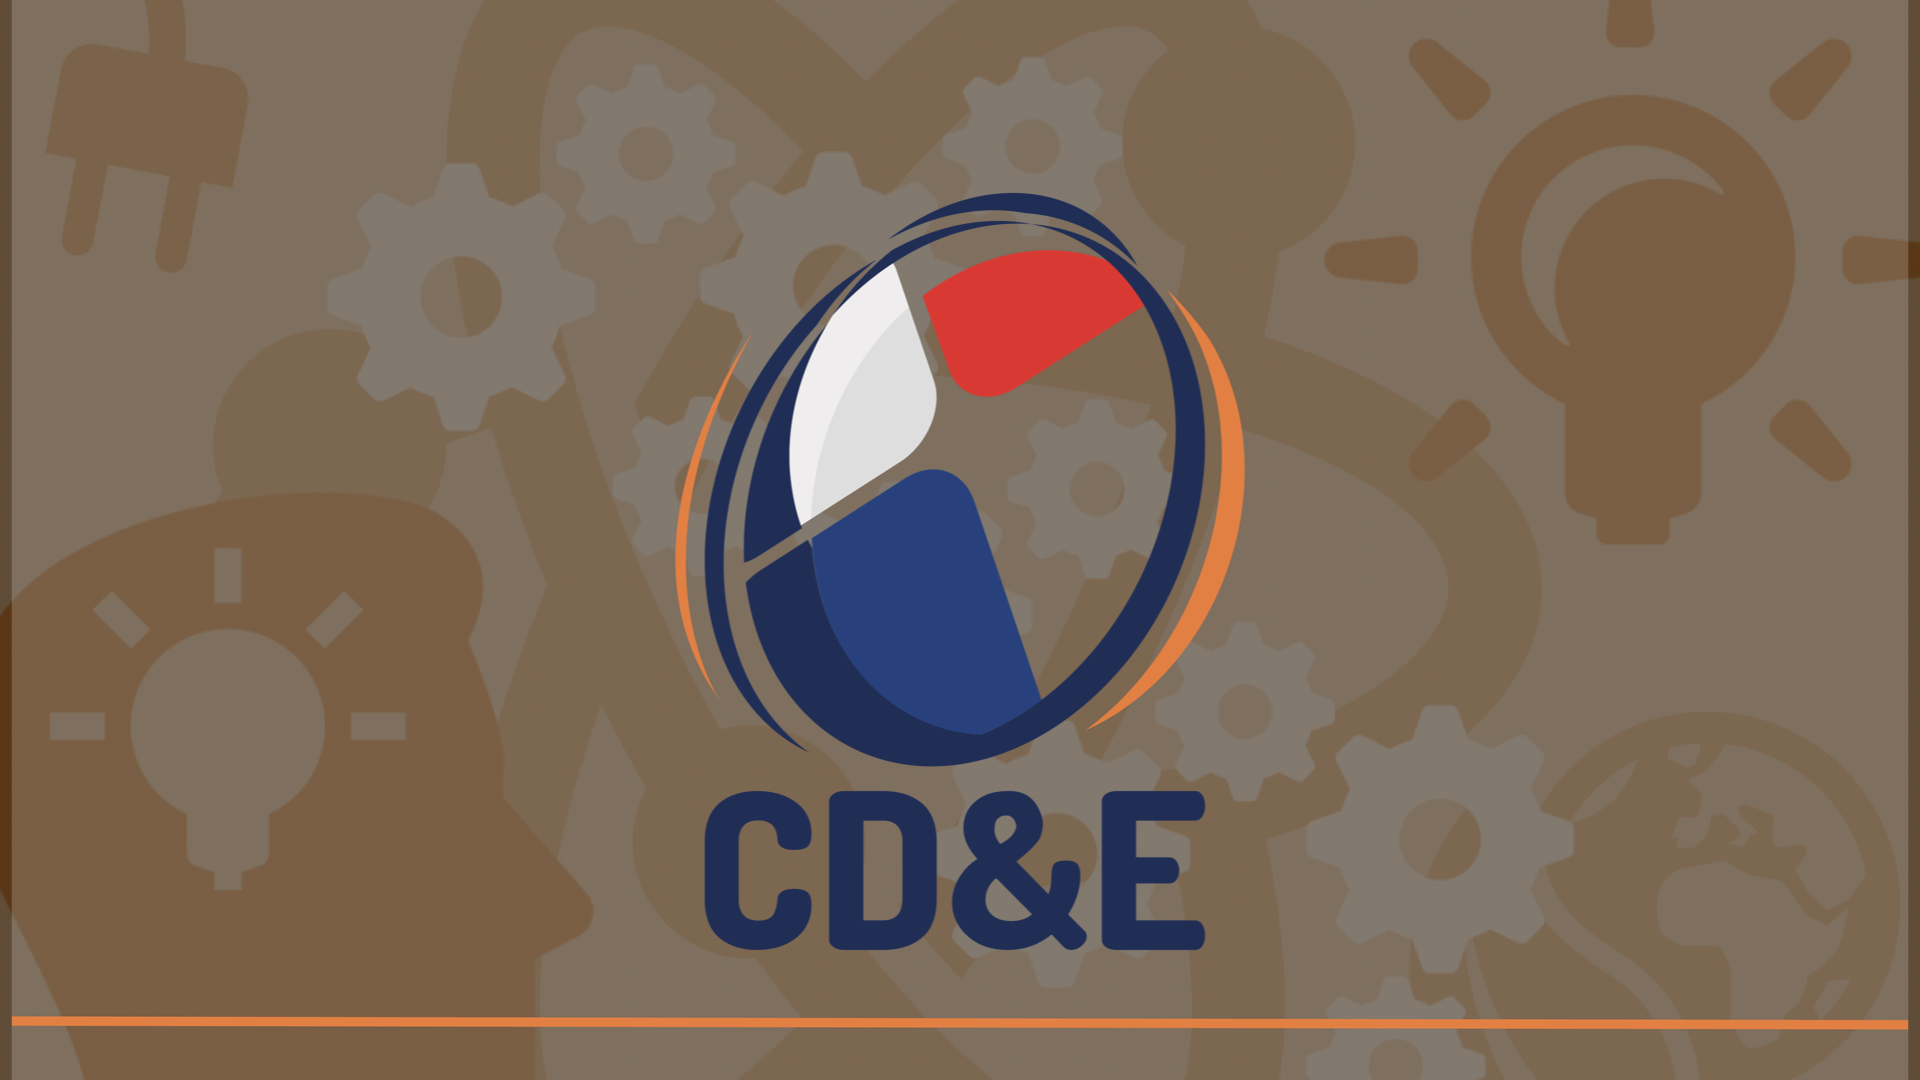
\includegraphics[width=26.67in]{data/keynote-slides/20200430-CDE-Designprocess/20200430-CDE-Designprocess.001} \caption{ }\label{fig:unnamed-chunk-2}
\end{figure}

\hypertarget{benaming}{%
\section{benaming}\label{benaming}}

De naam van ons team en methode is een aantal keer veranderd. We stonden bekend als CD\&E en worden op dit moment de afdeling Innovatie (i.o.) genoemd. Onze methodieken worden weleens benoemd als: CD\&E, kort-cyclisch moderniseren of -innoveren, trajectbegeleiding en programmatische aanpak. Ik zie vooral een `craft' ontstaan waarin deze methode en onze technieken en tools worden gehanteerd door `craftsman.' Ik noem deze `craft' Military Design \& Innovation.

Wat onder de craft Military Design \& Innovation wordt verstaan zal ik in de nabije toekomst beschrijven in dit boek. Dit boek wordt ook nog geredigeerd zodat eenduidige bewoording wordt gegeven aan de afdeling, methode, technieken en tools.

\hypertarget{aanleiding}{%
\section{aanleiding}\label{aanleiding}}

De reden om als Landmacht te innoveren met externe partners ligt in de realiteit dat een leger altijd beter moet zijn dan de tegenstander maar legers niet langer de innovatie aanjagen. De markt en economische marktwerking heeft dit overgenomen. En daar waar de Landmacht het idee had de ontwikkelingen voldoende te kunnen volgen, kreeg de Commandant Landstrijdkrachten de spiegel voorgehouden door de voorzitter/directeur van werkgeversorganisatie FME-CWM tijdens de Future Force Conference in 2015. De Landmacht pakte deze reflectie serieus aan en zoekt met externe organisaties naar samenwerking om in het tempo van de markt te innoveren in het landoptreden. De Landmacht gebruikte hierbij ondermeer de methode Concept Development \& Experimentation (CD\&E) als startpunt voor deze zoektocht.

CD\&E starte in 2015 als zogenaamde kwartiermakersgroep en maakte naam als afdeling, methode en resources voor kort cyclische moderniseren in het landoptreden. Sinds oktober 2017 mag ik bijdragen aan de missie van CD\&E. Startend als algemeen stafofficier junior ontwikkelde we met een klein team een methode, proces, tools en concept waarmee we kenniscentra en parate eenheden in staat konden stellen hun ideeën, en problemen om te zetten in vraagstukken die samen met interne en externe partijen middels experimenten worden beantwoord en ---als ultieme doel--- formeel opgenomen in de organisatie (implementatie). Deze aanpak is geen nieuw format of procedure maar een continue leerproces waarin samen wordt gewerkt aan nieuwe denkmodellen, activiteiten-pallet en craftmanship.

Veel van de CD\&E-aanpak is door de groei, successen (en mislukkingen) en de omgeving verandert, verbeterd of doorontwikkeld. Ook onstaan er nieuwe methode, processen, tools en concepten die de mogelijkheden voor innovatie in het landoptreden vergroten. Al deze nieuwe inzichten en handelingsperspectieven worden omgezet in kennis en vaardigheden die worden geborgt en gedeelt. Deze inspanningen dragen daarmee bij aan de missie.

\hypertarget{missie}{%
\section{missie}\label{missie}}

\begin{quote}
CD\&E ontsluit het innovatieve vermogen van het bedrijfsleven en kennisinstituten voor het moderniseringsproces van de Land- en/of Krijgsmacht zodat onze eenheden tijdens inzet relevant en waar nodig dominant blijven.
\end{quote}

In het vakgebied Military Design \& Innovation borgen en delen we de kennis en vaardigheden in de exploratie van ambities, idee-generatie, vraagarticulatie, samenwerking met externe partijen en implementatie van nieuwe capablities.

\hypertarget{beleid}{%
\section{beleid}\label{beleid}}

\begin{figure}
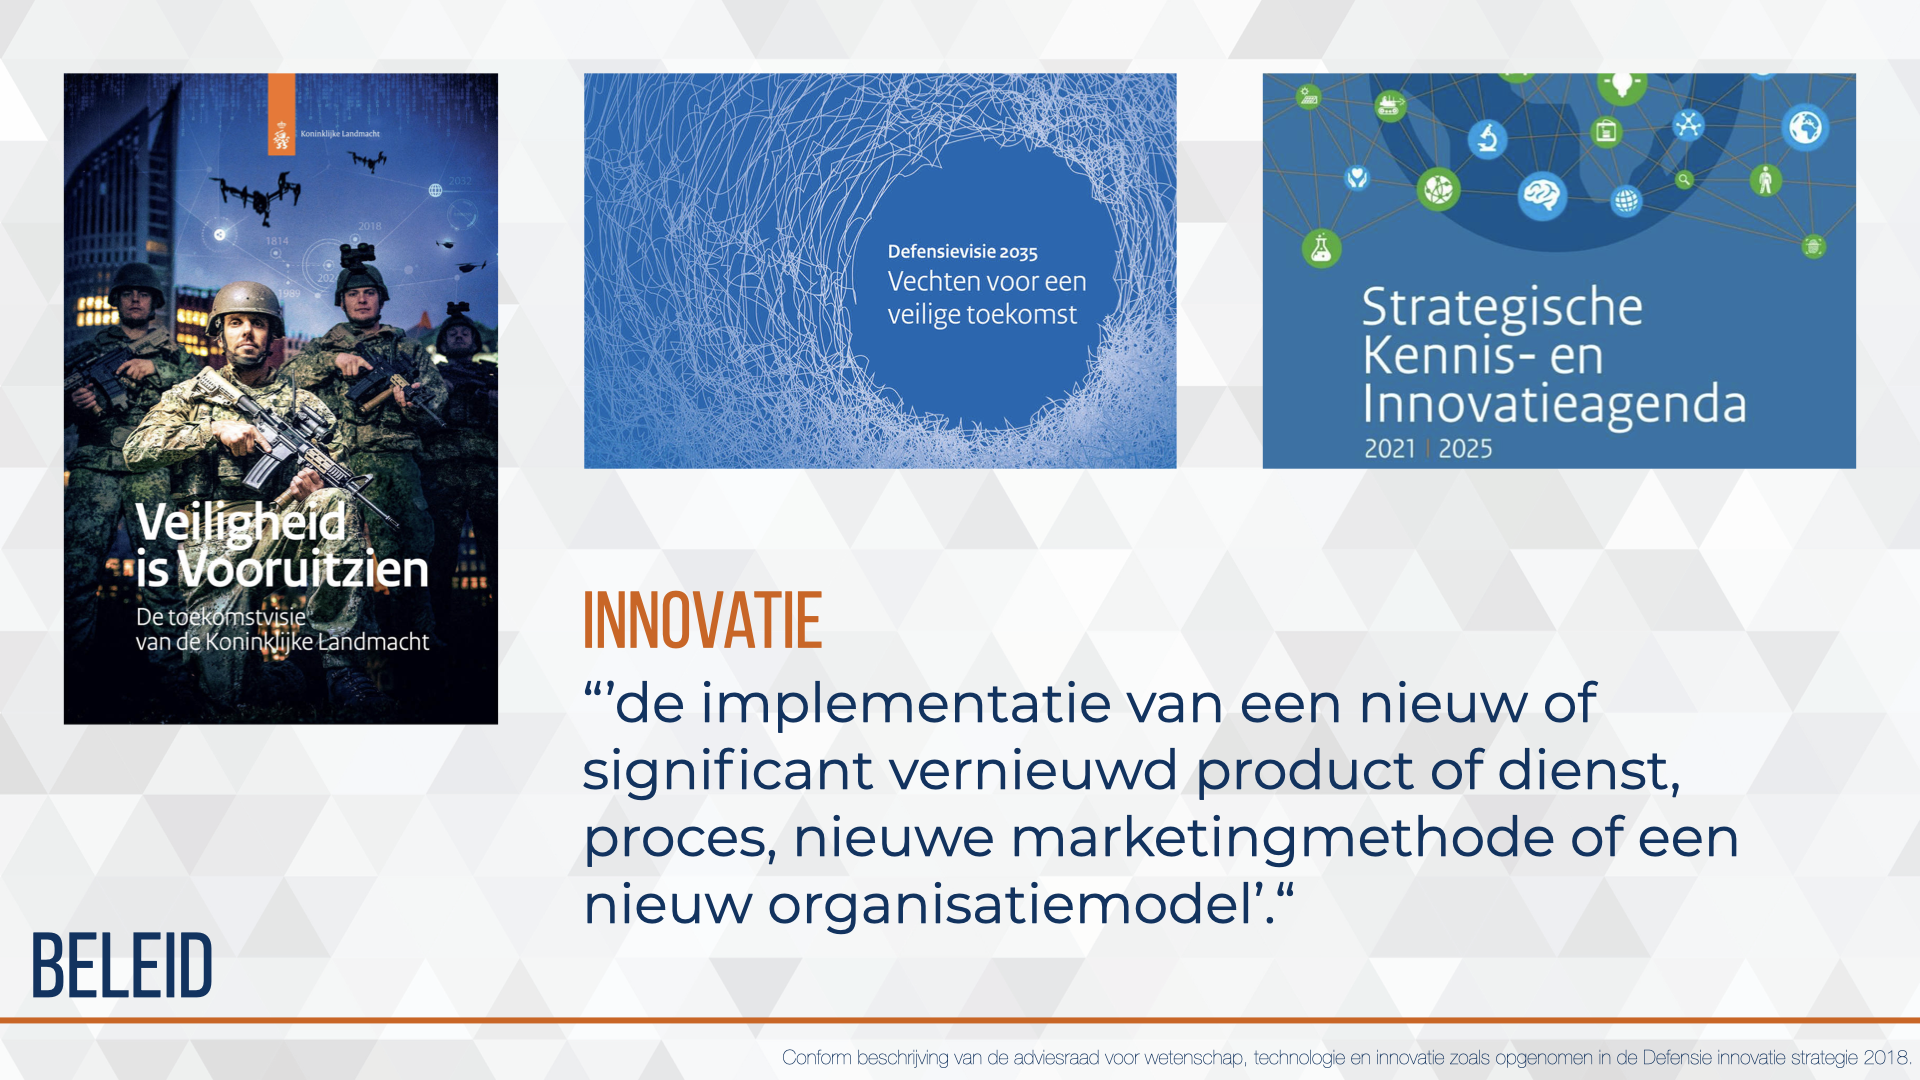
\includegraphics[width=26.67in]{data/keynote-slides/20200430-CDE-Designprocess/20200430-CDE-Designprocess.005} \caption{ }\label{fig:unnamed-chunk-3}
\end{figure}

Er zijn een aantal beleidsdocumenten die het moderniseren en innoveren van de Land- en Krijgsmacht sturen. Drie documenten komen met enige regelmaat terug. De Defensievisie 2035, Vechten voor een veilige toekomst beschrijft de inrichtingsprincipes voor de eerstkomende jaren. De Strategische kennis- en innovatieagenda geeft meer thematisch aan in welke onderwerpen Defensie de focus legt. De Visie Commando Landstrijdkrachten, Veigligheid is vooruitzien, beschrijft het toekomstbeeld van de Kominklijke Landmacht. Deze is intern verder vertaald in het Operationeel kader landoptreden (OKL).

Als definitie voor innovatie volg ik de Adviesraad voor Wetenschap, Technologie en Innovatie.

\begin{quote}
Innovatie: ``de implementatie van een nieuw of significant vernieuwd product of dienst, proces, nieuwe marketingmethode of een nieuw organisatiemodel.`` (\protect\hyperlink{ref-awti-2014}{Adviesraad voor het Wetenschaps- en Technologiebeleid, 2014})
\end{quote}

\hypertarget{uitgangspunten}{%
\section{uitgangspunten}\label{uitgangspunten}}

Bij het ontwikkelen van een modellen en processen zijn er een aantal zaken waar de Landmacht rekening mee moet houden. Bij wet kent de Landmacht een aantal verplichtingen zoals de wijze waarop partners en leveranciers worden geselecteerd of de manier waarop geld wordt uitgegeven.

Daarnaast kent de organisatie een snelle doorstroom van functionarissen en dwingende processen en regels.
Functionarissen doen wat zij kennen, weten en wat de afdeling of eenheid gewoon is te doen vanuit de intentie kwaliteit te willen leveren als vakmensen. Door de snelle doorstroom is het lastig de mogelijkheden van de wet- en regelgeving ten volle te benutten.
Procedures maken de gang van zaken controleerbaar, repeteerbaar en voorspelbaar maar vooral borgt het de sociale waarden van de Landmacht als overheidsorganisatie.

Dit resulteert in drie uitgangspunten die kaderstellend zijn bij het doorontwikkelen van modellen, processen en instrumenten voor Military Design \& Innovation.

\textbf{Landmacht is een aanbestedende dienst}
dus moeten inkoop en verwerving voldoen aan Europese wetgeving.

\textbf{Landmacht is een rijksoverheidsorganisatie}
met een Ministeriële verantwoording aan parlement over verantwoorde uitgave van belastinggeld en handelen naar de Nederlandse overtuigingen en belangen.

\textbf{Landmacht is een bureaucratische organisatie}
waarin processen en regelgeving borgen dat de organisatie non-discriminatief handelt conform Weber's model.

\hypertarget{moderniseringsmodellen}{%
\section{moderniseringsmodellen}\label{moderniseringsmodellen}}

Voor de lang-cyclische modernisering kent de Landmacht het CLAS moderniseringsmodel waar vanuit een future scan (landoptreden van de toekomst LvT) wordt toegewerkt naar een force design (Landmacht van overmorgen LvOM), force building (Landmacht van morgen LvM) en force employment (Landmacht van vandaag LvV).

\begin{figure}
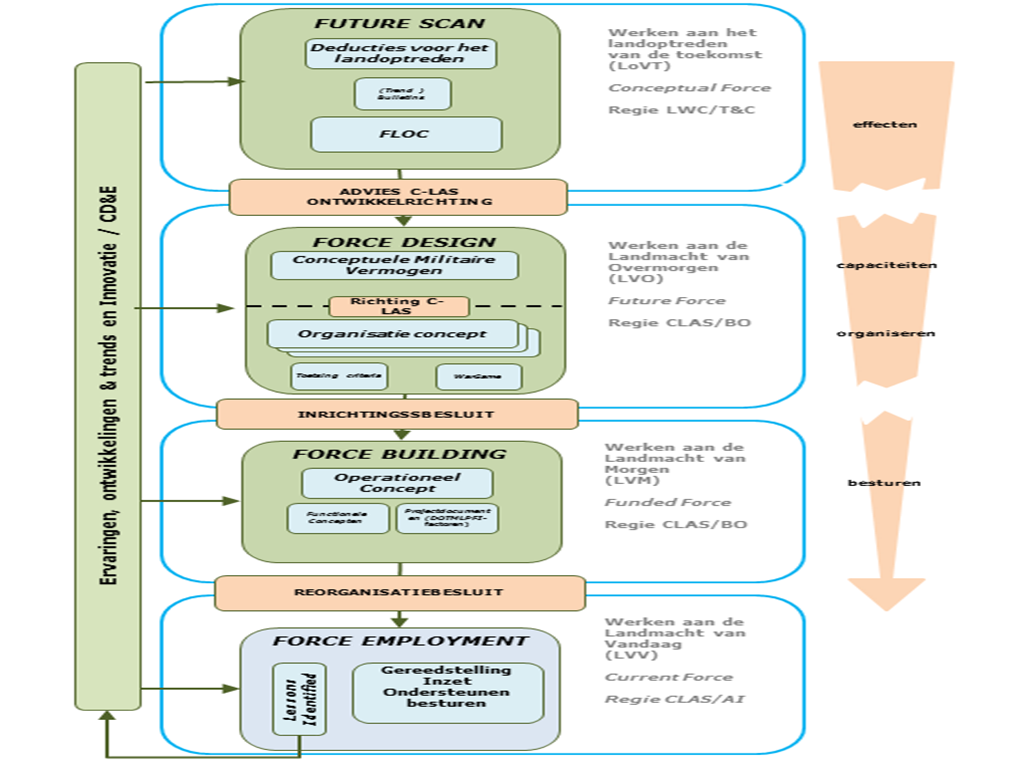
\includegraphics[width=14.29in]{data/images/BO-2016-CLAS-moderniseringsmodel} \caption{CLAS moderniseringsproces lang-cyclisch }\label{fig:unnamed-chunk-4}
\end{figure}

Defensie breed is de lang-cyclische modernisering en innovatie ingericht als een `huis.' Dit kennis- en innovatie model is al jaren in gebruik en voorziet in vele instrumenten en processen om innovatie op lange termijn toe te passen. Echter het gebruiken van nieuwe snel opkomende innovaties kunnen hiermee niet adequaat worden getest en geïmplementeerd.

\begin{figure}
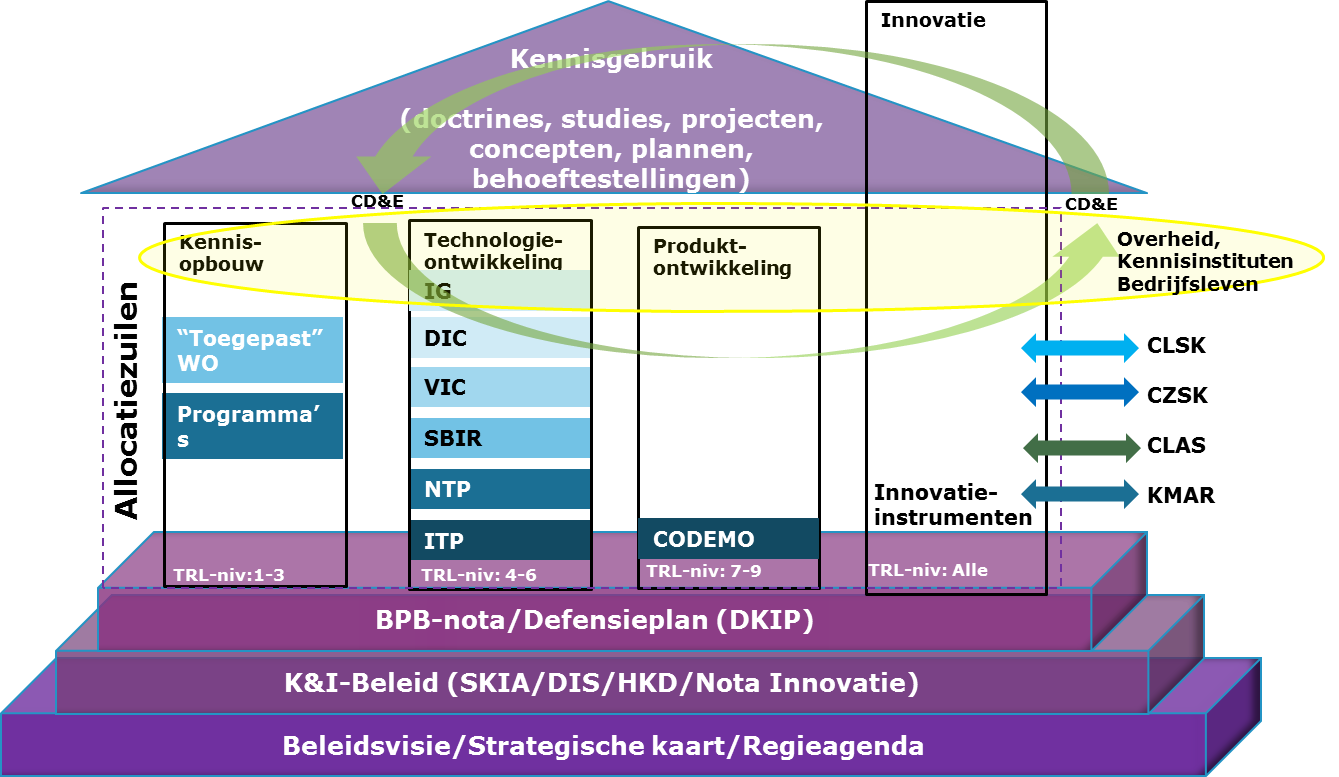
\includegraphics[width=18.6in]{data/images/BO-2016-Defensie-KI-huis} \caption{Visuele weergave van het kennis \& innovatiehuis Defensie}\label{fig:ki-test}
\end{figure}

Met CD\&E werkt de Landmacht sinds 2015 aan het versnellen, verbinden en vermarkten van opkomende technologieën en ambities door het organiseren en structureren van innovatie in het tempo van de markt.

\hypertarget{cde-binnen-clas-modernisering}{%
\subsection*{CD\&E binnen CLAS-modernisering}\label{cde-binnen-clas-modernisering}}
\addcontentsline{toc}{subsection}{CD\&E binnen CLAS-modernisering}

\begin{figure}
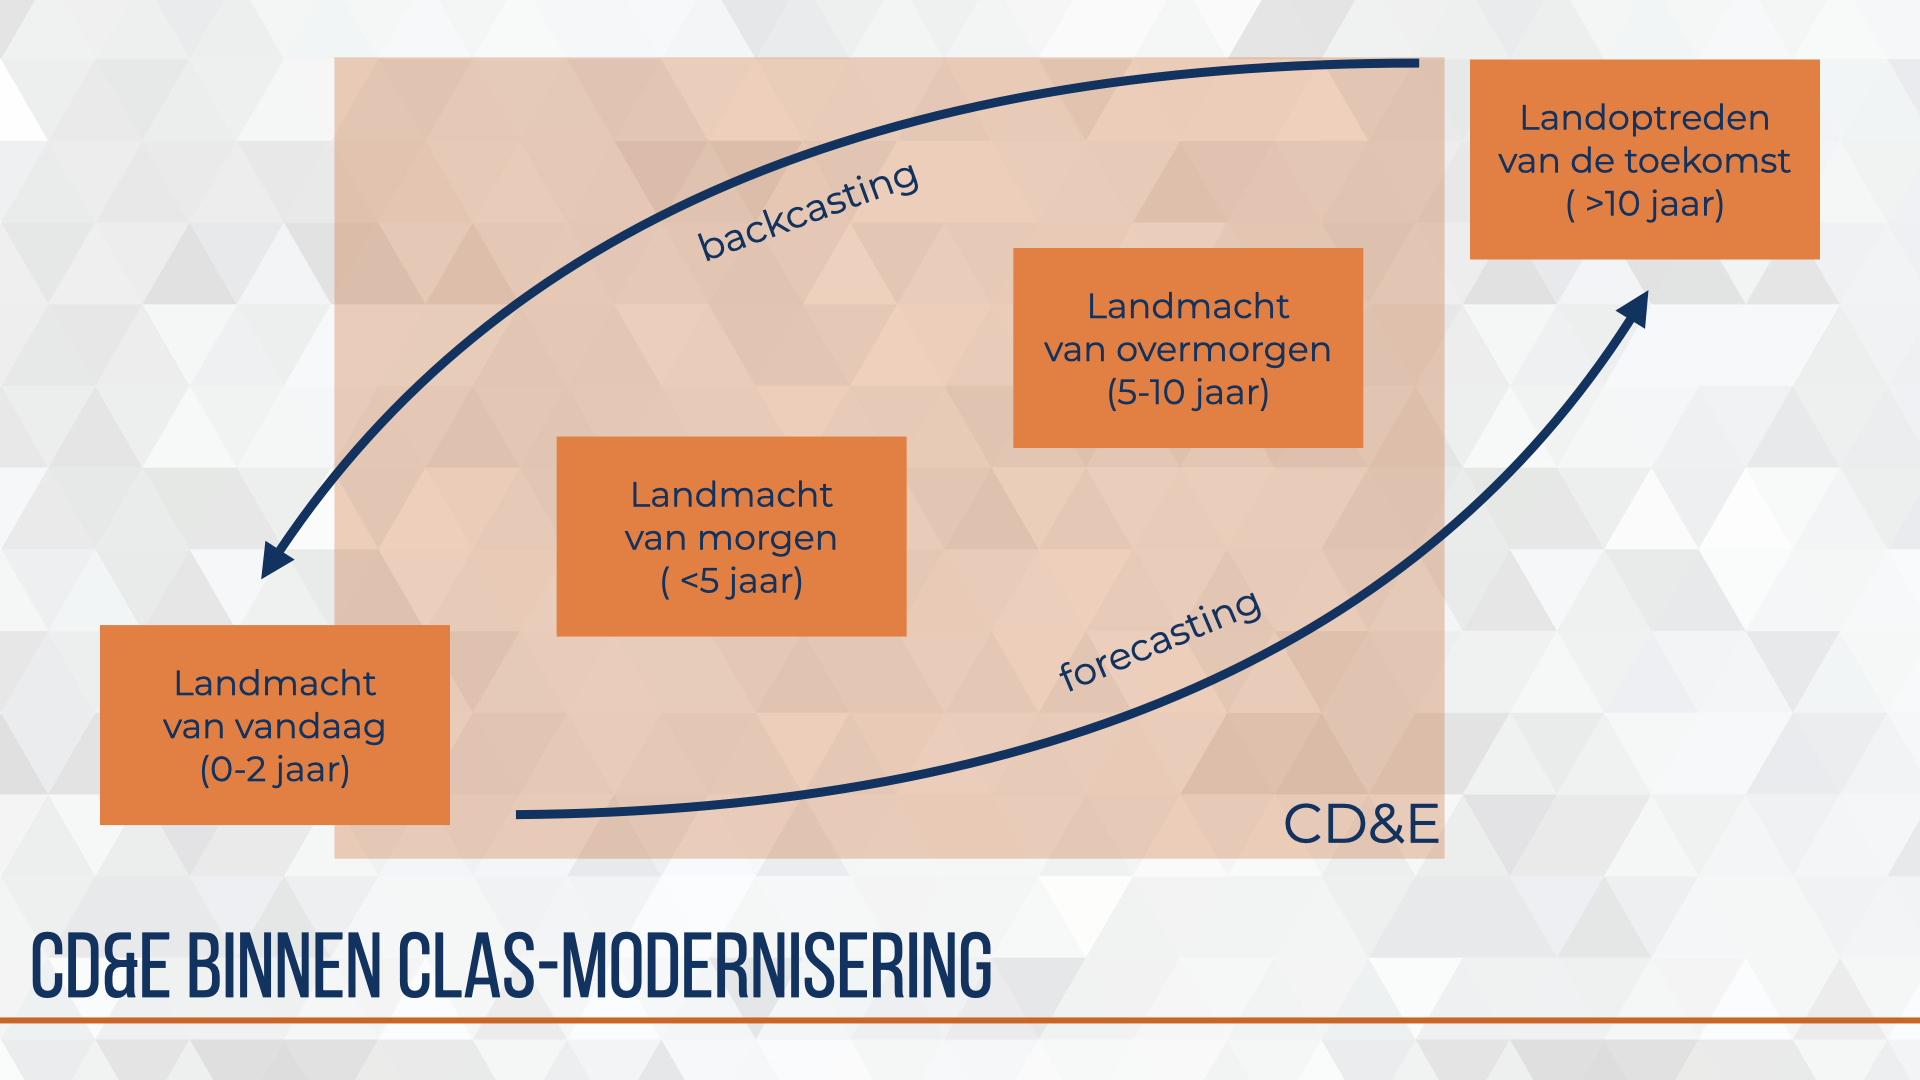
\includegraphics[width=26.67in]{data/keynote-slides/20200430-CDE-Designprocess/20200430-CDE-Designprocess.008} \caption{Eenvoudig CLAS moderniseringsproces met positionering van de CD\&E-methodiek}\label{fig:simpel-proces}
\end{figure}

Figuur \ref{fig:simpel-proces} en vereenvoudigde visualisatie van het `klassieke' moderniseringsproces van de Landmacht. Dit proces kan worden onderverdeeld in vier aandachtsgebieden, de landmacht van vandaag (LvV), morgen (LvM), overmorgen (LvOM) en het landoptreden van de toekomst (LvT). Verschillende organisatie-onderdelen dragen bij aan deze aandachtsgebieden. Grofweg kan de verantwoordelijkheid (responsibility) worden toebedeeld aan respectievelijk de parate eenheid, afdeling strategie \& plannen, kenniscentrum en afdeling trends \& concepts.
In dit proces vindt backcasting plaats doordat onderzoek, studies en verkenningen richting geven aan modernisering voor LvM en LvV en forecasting doordat evaluaties, lessons learned en experimenten richting geven aan beleid, budgettering en kennisplanning.

CD\&E draagt hoofdzakelijk bij aan de landmacht van morgen en overmorgen.

\hypertarget{cde-algemeen}{%
\chapter{Organisatie}\label{cde-algemeen}}

\hypertarget{positionering-in-defensie-organisatie}{%
\section{positionering in defensie organisatie}\label{positionering-in-defensie-organisatie}}

\begin{figure}
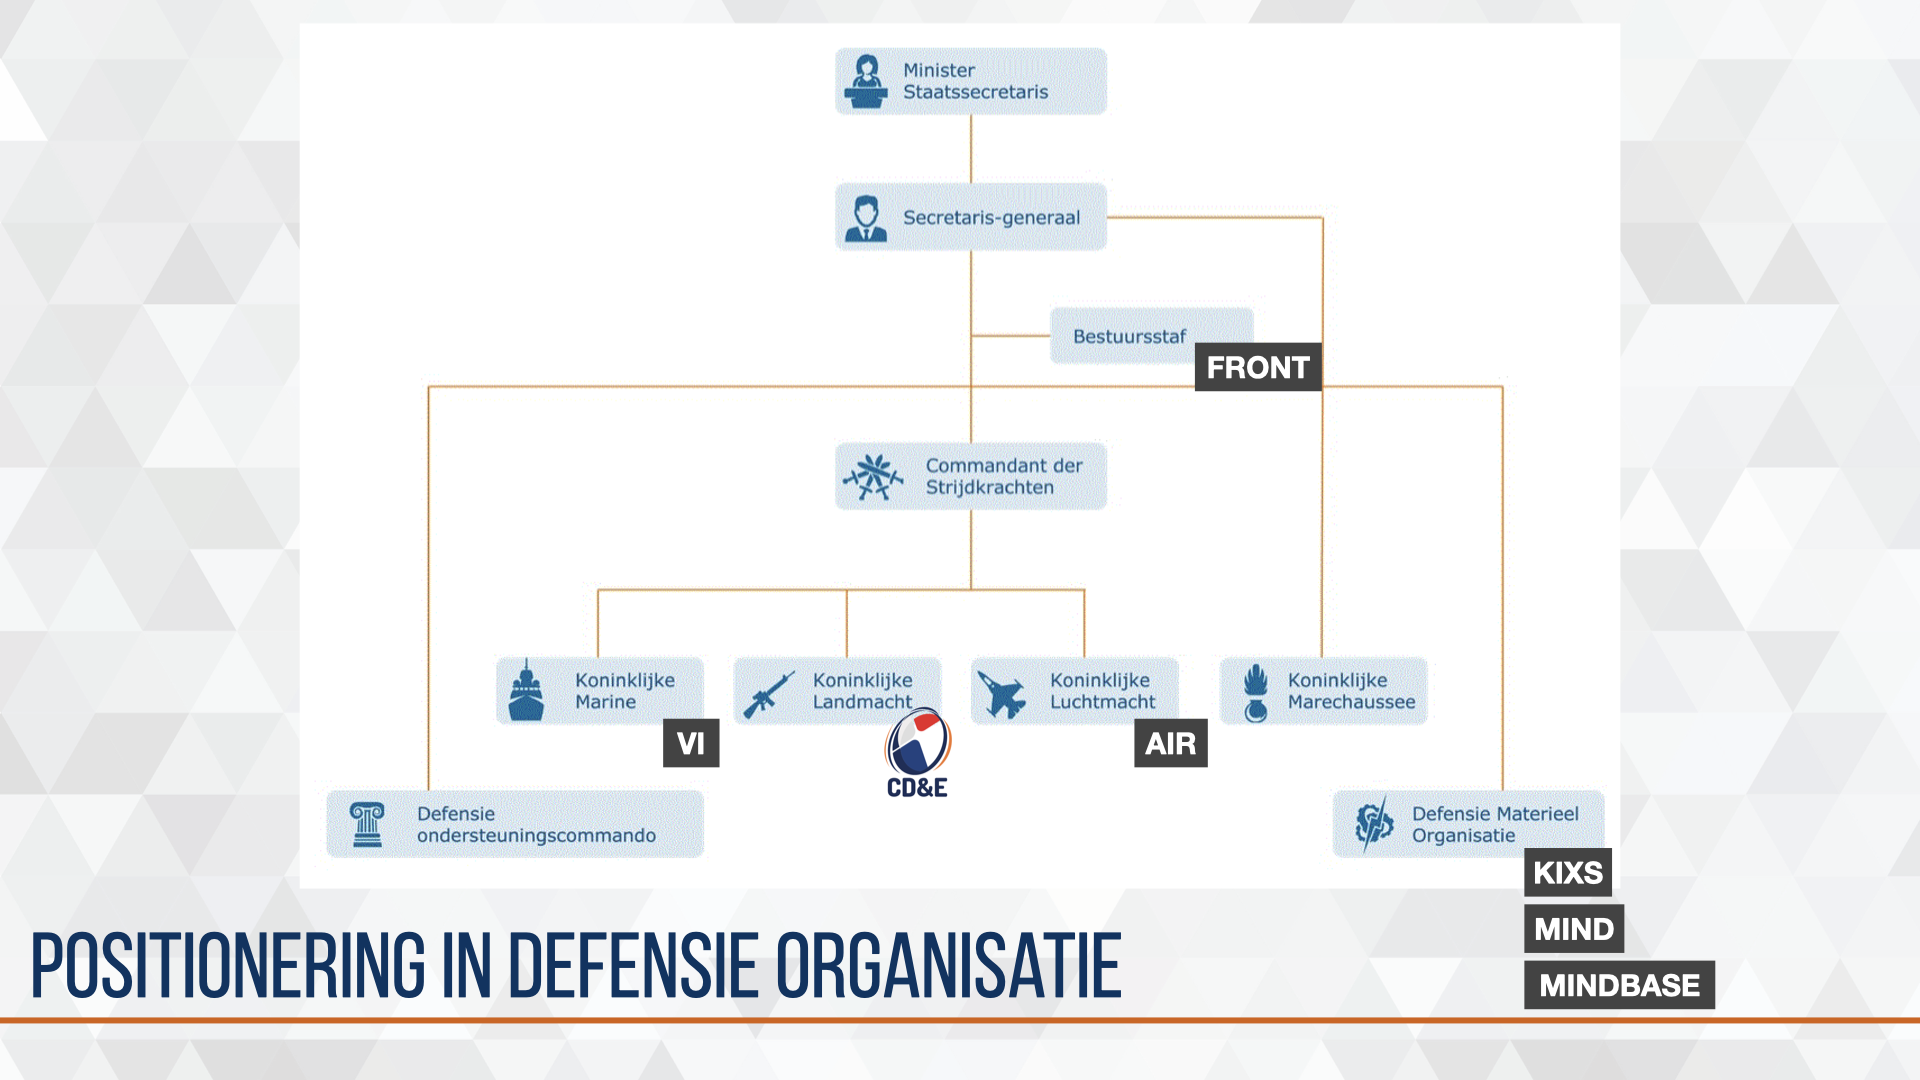
\includegraphics[width=26.67in]{data/keynote-slides/20200430-CDE-Designprocess/20200430-CDE-Designprocess.009-1} \caption{Positionering innovatiecentra binnen Defensie }\label{fig:unnamed-chunk-6}
\end{figure}

CD\&E is het innovatiecentrum van de Landmacht. Ook de andere defensieonderdelen kennen innovatiecentra, ieder opgebouwd in de kenmerken en cultuur van het defensieonderdeel.

\hypertarget{organisatorische-ontwikkelingen}{%
\section{organisatorische ontwikkelingen}\label{organisatorische-ontwikkelingen}}

\hypertarget{organisatie-2019-multi-project-management}{%
\subsection{organisatie 2019: multi-project management}\label{organisatie-2019-multi-project-management}}

\begin{figure}
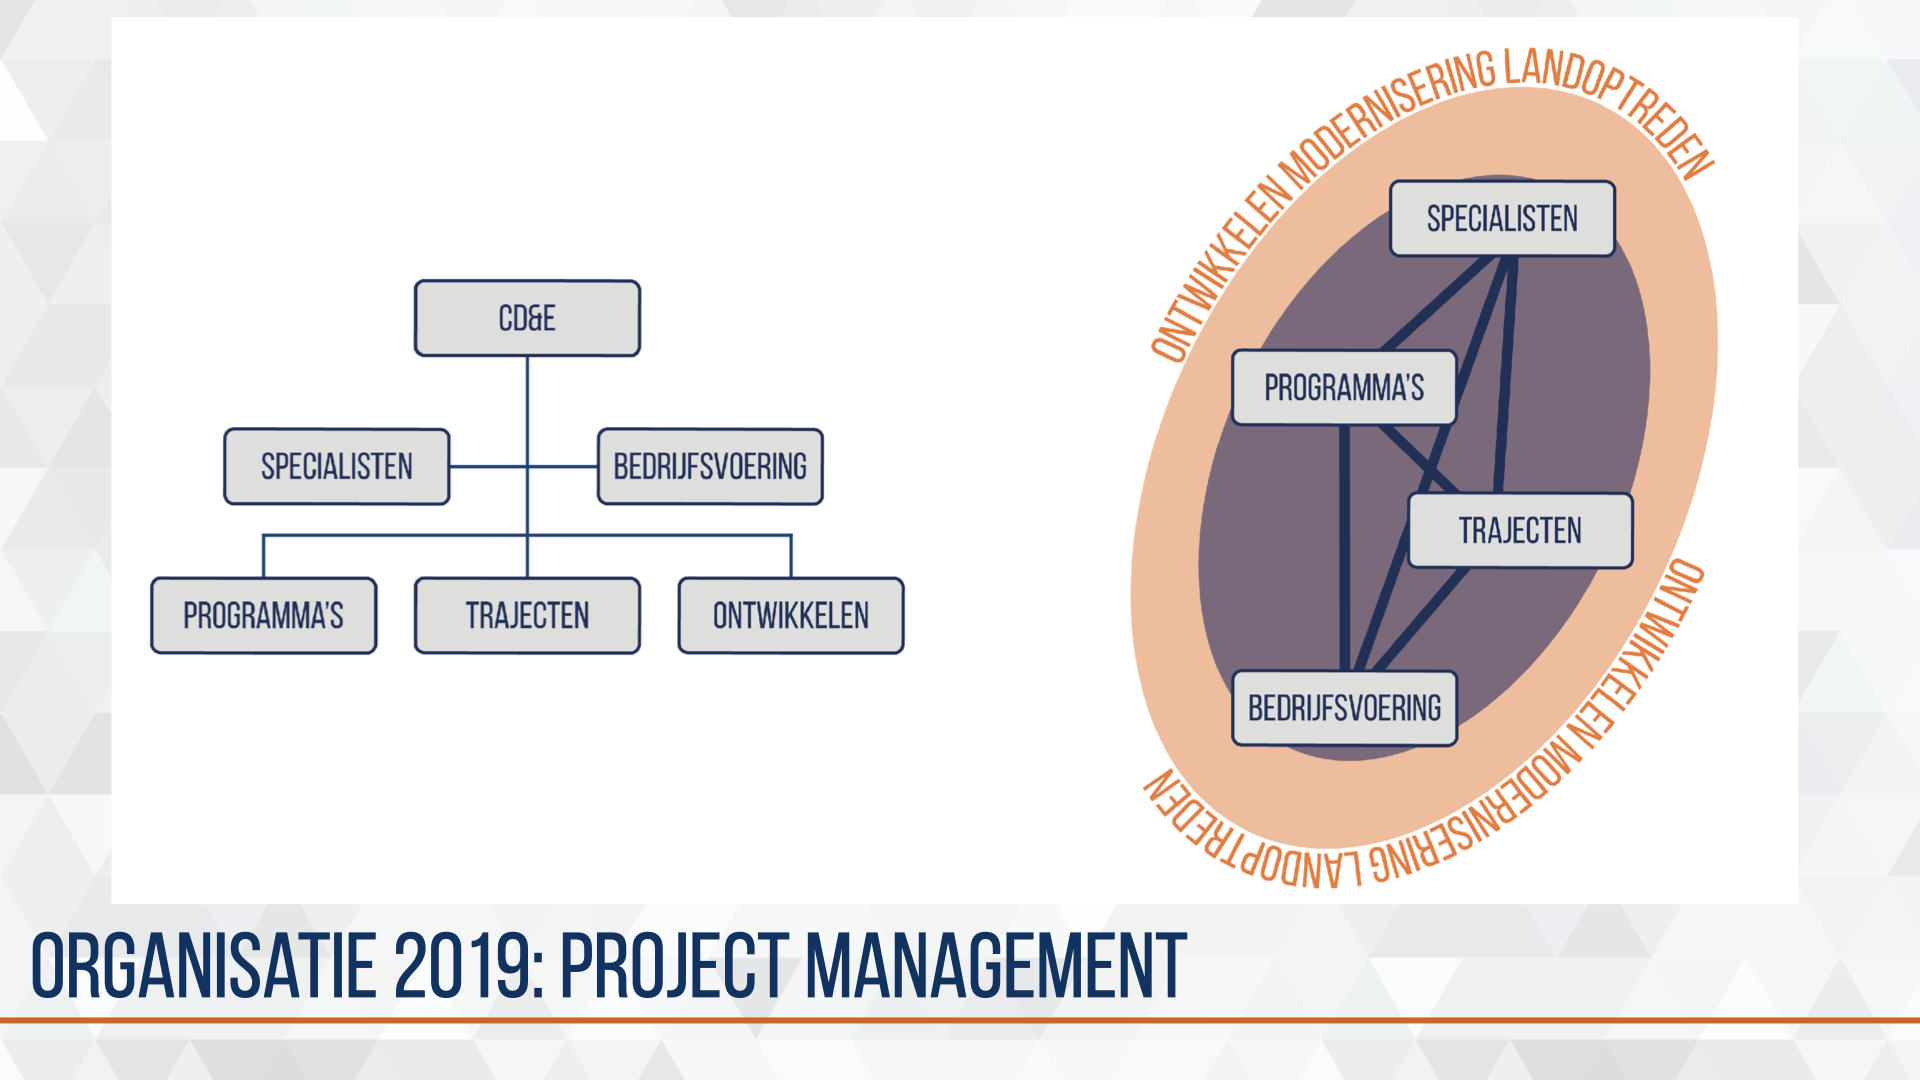
\includegraphics[width=26.67in]{data/keynote-slides/20200430-CDE-Designprocess/20200430-CDE-Designprocess.009-2} \caption{Organisatie structuur voor multi-project management }\label{fig:unnamed-chunk-7}
\end{figure}

In 2019 groeide het team dusdanig dat enige verdeling en specialisatie onvermijdelijk werd. Teams werden ingericht naar activiteiten en het niveau waarop hoofdzakelijk werd gesteund.

Trajecten groepeerde de trajectbegeleiders en werkte voornamelijk met de kenniswerkers (kennis- en expertise centra) en stafmedewerkers (parate eenheid).

Binnen Programma's zaten programma-managers die de kennisadviseurs (commandanten van opleiding- en trainingscentra) en dossierhouders (afdeling Strategie en Plannen) steunde in het opzetten van routekaarten van operationele wensen en behoefte.

Ontwikkelen was gericht op de strategische inbedding van alle inspanningen.

Bedrijfsvoering behelst alle CD\&E ondersteunende processen, uitvoering van evenementen en logistieke ondersteuning.

De vele individuele of specifieke teamleden werden onder Specialisten geschaard.

De aanpak is een olievlekwerking. Met trajecten en programma's creëren we voorbeelden waardoor operationele en bedrijfsmatige knelpunten zichtbaar worden zodat deze geadresseerd kunnen worden bij de juiste entiteiten. Dit draagt bij aan het structureel kort-cyclisch moderniseren in het landoptreden.

\hypertarget{transitie-2020}{%
\subsection{transitie 2020}\label{transitie-2020}}

\begin{figure}
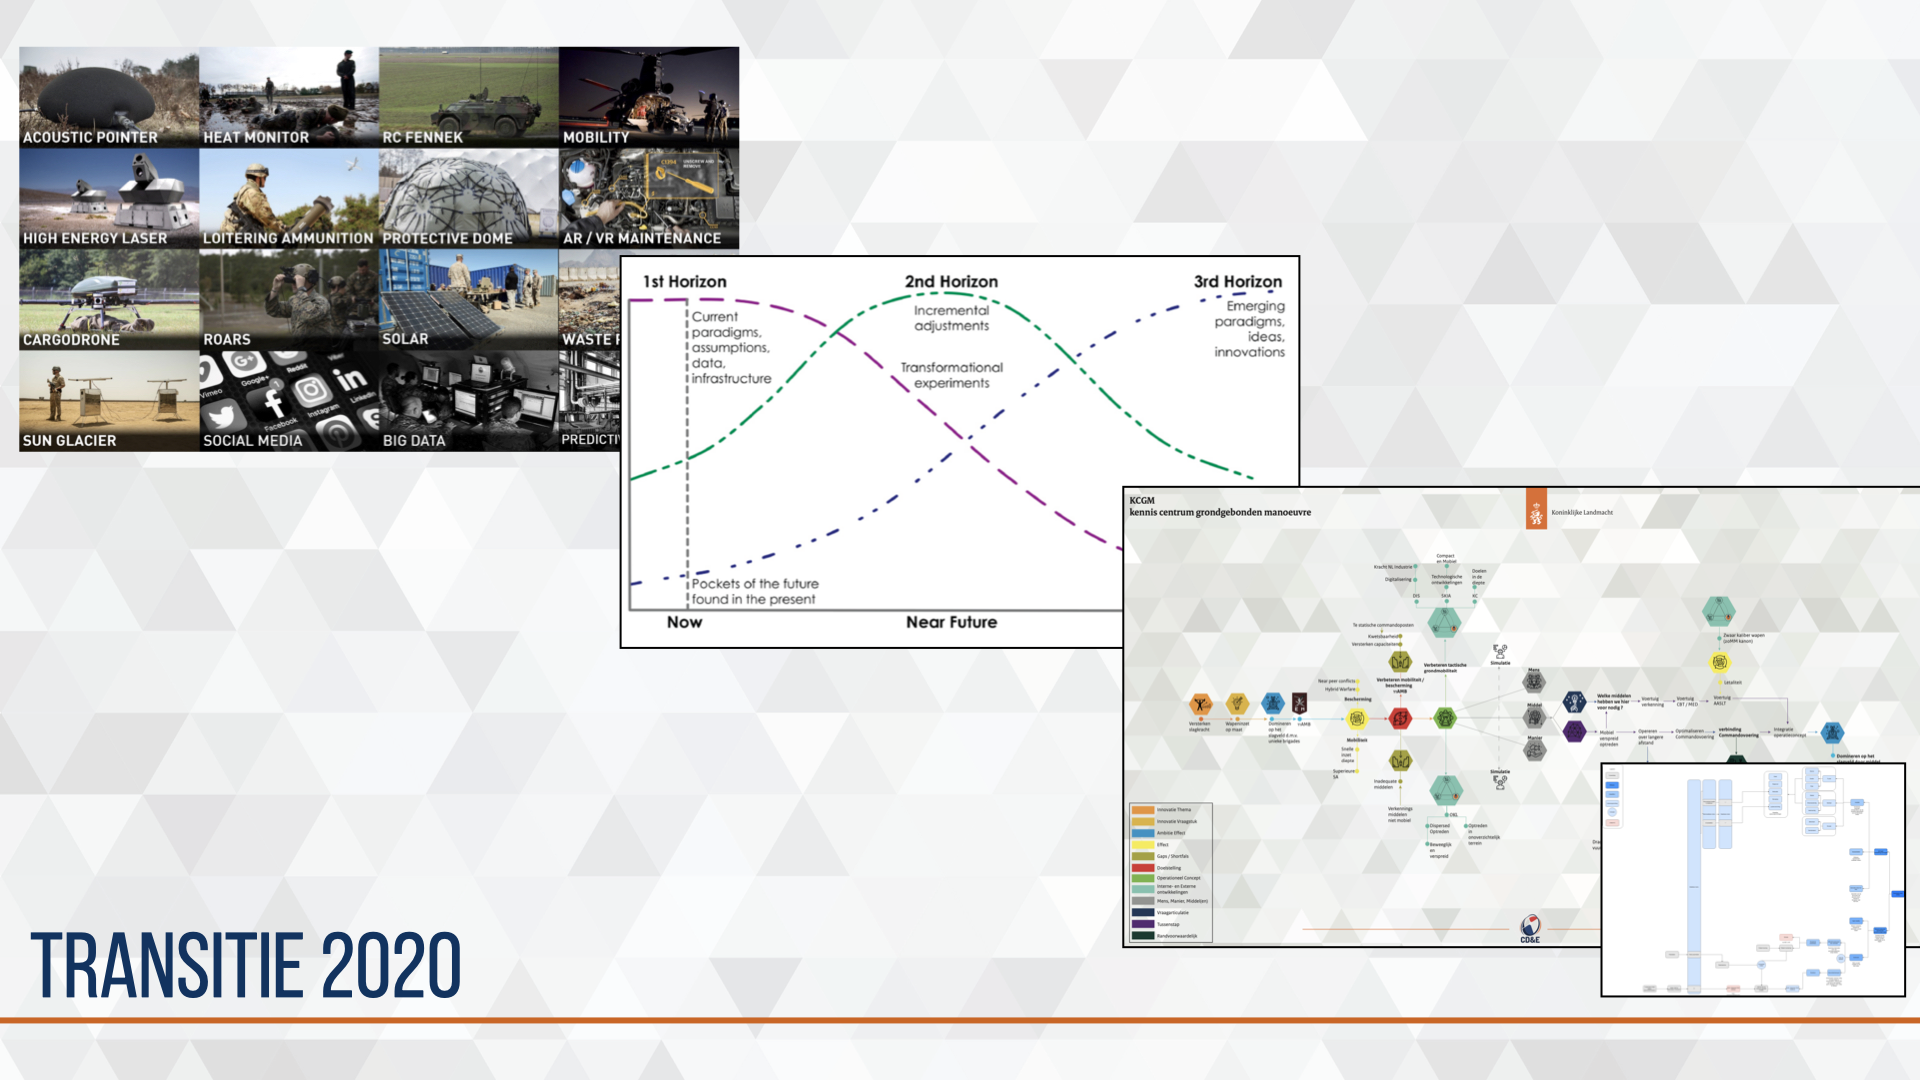
\includegraphics[width=26.67in]{data/keynote-slides/20200430-CDE-Designprocess/20200430-CDE-Designprocess.009-3} \caption{Van multi projecten via 3-horizon model naar routekaarten.}\label{fig:unnamed-chunk-8}
\end{figure}

In 2020 deden we een herijking op het project portfolio zodat de focus blijft op de juiste initiatieven. Deze herijking was een staf integraal proces waarin projecten werden beschouwd op relevantie, urgentie, noodzaak en realiseerbaarheid binnen het landoptreden. De herijking maakte de vele initiatieven inzichtelijk en keuzen door Directeur Kennis \& Ontwikkeling mogelijk. De multi-project aanpak creëerde daarmee een vorm van overzicht, inzicht en regie. (Foto brownpaper nog toevoegen)

Het werd tijd voor de volgende stap waarin meer richting wordt gegeven aan de initiatieven vanuit ambitie, markt tempo en markt potentieel. De programmatische aanpak werdt daarvoor gekozen. Programma-managers inventariseren moderniseringsinitiatieven bij de 9-14 kennisadviseurs m.b.v. Boill Sharp's 3-horizon model en visualiseren deze initiatieven in een hiërarchie-boom-structuur die routekaart werd genoemd.

\hypertarget{organisatie-2021-programma-management}{%
\subsection{organisatie 2021: programma management}\label{organisatie-2021-programma-management}}

\begin{figure}
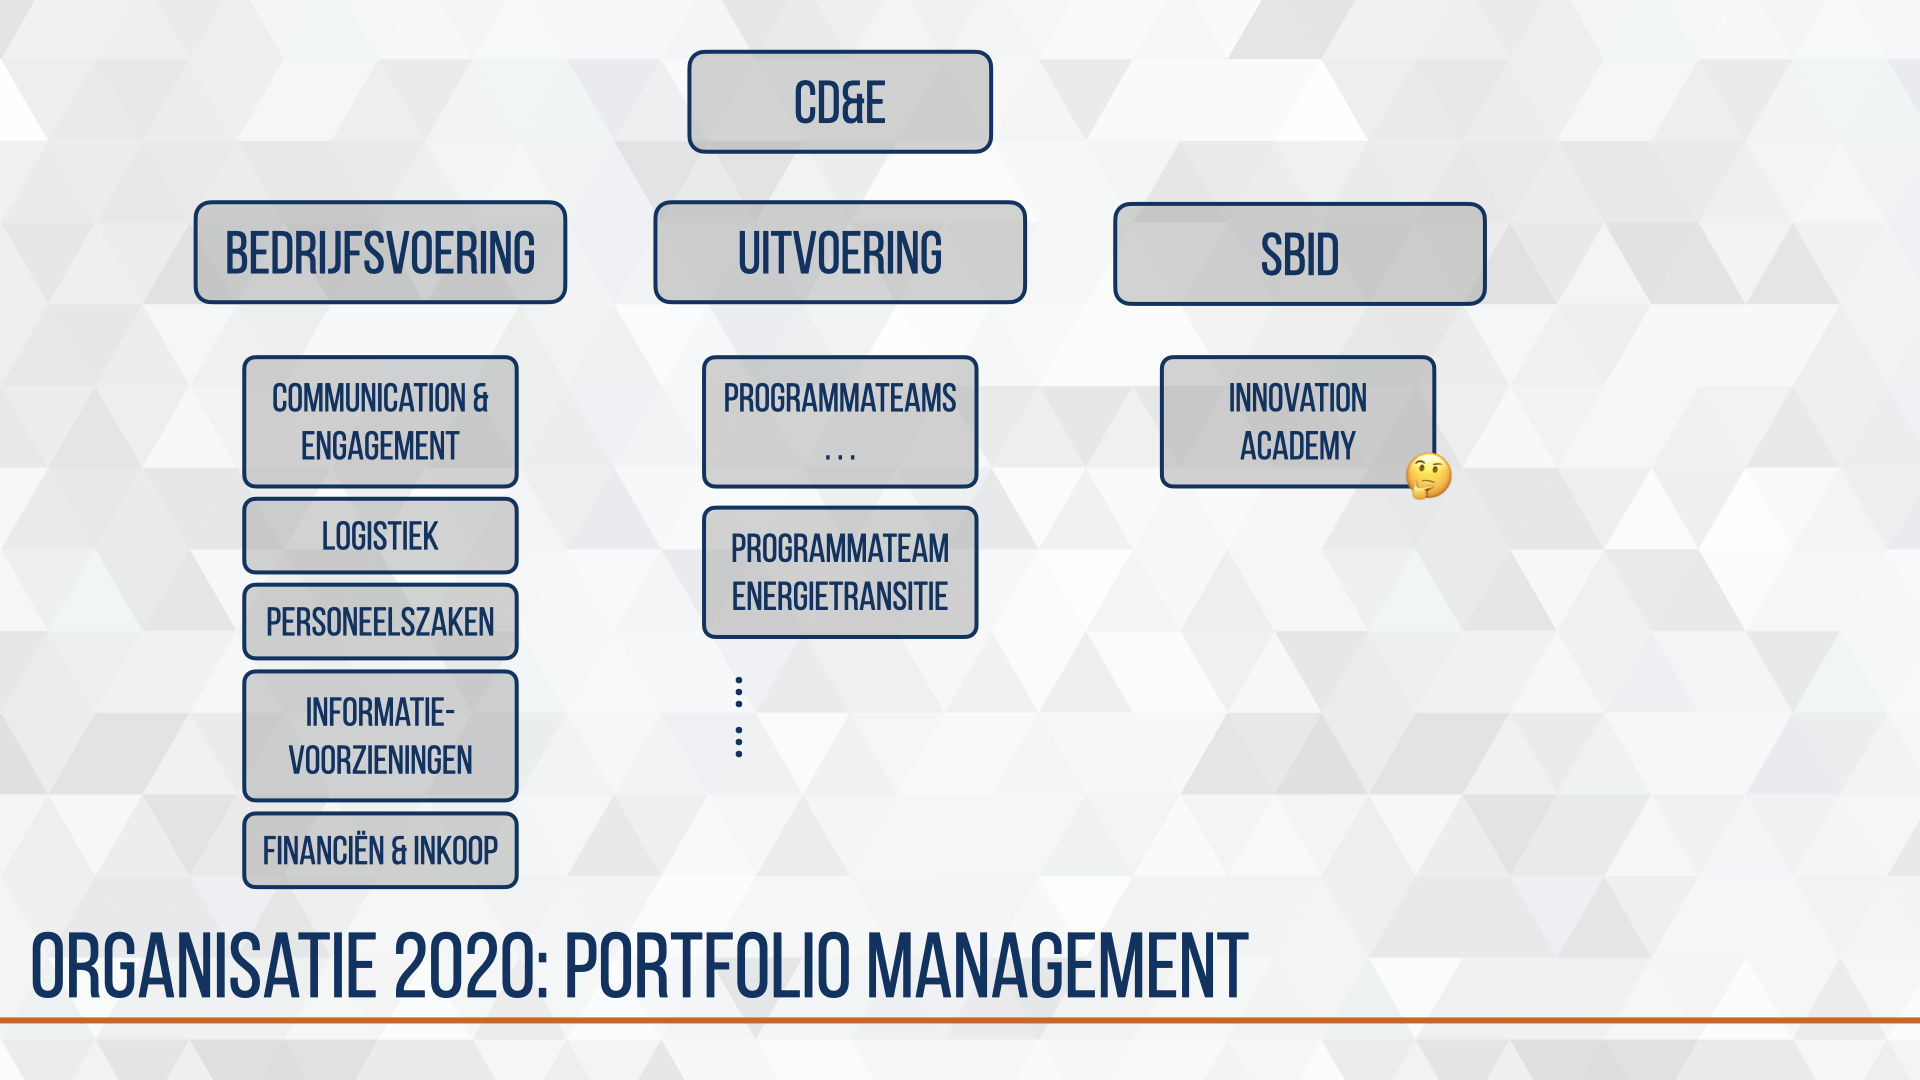
\includegraphics[width=26.67in]{data/keynote-slides/20200430-CDE-Designprocess/20200430-CDE-Designprocess.009-4} \caption{Organisatie structuur naar programmatische aanpak }\label{fig:unnamed-chunk-9}
\end{figure}

In 2020 groeide CD\&E uit tot een volwaardige innovatie partner, werden CD\&E en DAK-C samengevoegd in een Afdeling Innovatie onder de Directie Kennis \& Ontwikkeling, consolideerde het budget, werden de moderniseringsvraagstukken groter en complexer en werd zichtbaar en merkbaar voortgang geboekt met strategische inbedding.

Het was tijd om opnieuw de structuur en benadering aan te passen. Programma-management is de gekozen aanpak omdat dit planbaar en beheersbaar is in de interne bedrijfsvoering en herkenbaarheid en vertrouwen creëert in de samenwerking met externe partners (koepelorganisaties, MKB-ers, kennisinstituten). Er worden daarom hoofd-programma's geformeerd rondom een specifiek thema, hierin zitten verschillende moderniseringsprojecten. Een programmateam met programma-managers en trajectbegeleiders werken samen aan het hoofdprogramma.

Alle programma's komen onder Uitvoering terwijl de (door)ontwikkeling en strategische inbedding worden samengebracht bij Strategic Business \& Innovation Development (SBID). Er komst dus een scheiding tussen toekomst, uitvoering en ondersteuning.

\hypertarget{middelen}{%
\section{middelen}\label{middelen}}

De uitvoering van innovatieprojecten vindt plaats op locatie en in eigenaarschap van een kenniscentrum of parate eenheid, de afdeling Innovatie (io) steunt en faciliteert. Hiervoor heeft de afdeling Innovatie (io) een aantal middelen en diensten tbeschikbaar. Dit zijn de middelen en diensten die niet vanzelfsprekend toegankelijk zijn voor de betrokken partijen of vanwege schaarste of efficiëntie beter tot hun recht komen door centrale positionering.

\hypertarget{begeleiden-en-faciliteren}{%
\subsection{begeleiden en faciliteren}\label{begeleiden-en-faciliteren}}

De belangrijkste diensten van de afdeling Innovatie (io) zijn het begeleiden van de Landmacht-professionals bij het innoveren in hun vak en van hun vakmanschap. Daarom neemt de afdeling Innovatie (io) geen primair eigenaarschap in de programma's of projecten maar steunt de opdrachtgever, -nemer en overige betrokkenen in het gehele traject tot implementatie en escaleert naar de juiste niveaus waar nodig.

\hypertarget{rollen}{%
\subsubsection{rollen}\label{rollen}}

Het beschrijven van context, selecteren van activiteiten en betrekken van partners is eerder een kunst dan wetenschap. Deze kunst is het craftmanship van trajectbegeleiders, programma-managers en SBID-medewerkers. De verschillende rollen die bijdragen in een traject worden hier -in een later moment- beschreven. De kwaliteiten en kwalificaties van deze rollen volgen uit de doorontwikkeling Military Design \& Innovation 2021.

\hypertarget{trajectbegeleider}{%
\paragraph*{trajectbegeleider}\label{trajectbegeleider}}
\addcontentsline{toc}{paragraph}{trajectbegeleider}

\hypertarget{programma-manager}{%
\paragraph*{programma-manager}\label{programma-manager}}
\addcontentsline{toc}{paragraph}{programma-manager}

\hypertarget{sbid-medewerker}{%
\paragraph*{SBID-medewerker}\label{sbid-medewerker}}
\addcontentsline{toc}{paragraph}{SBID-medewerker}

\hypertarget{opdrachtgever}{%
\paragraph*{opdrachtgever}\label{opdrachtgever}}
\addcontentsline{toc}{paragraph}{opdrachtgever}

\hypertarget{opdrachtnemer}{%
\paragraph*{opdrachtnemer}\label{opdrachtnemer}}
\addcontentsline{toc}{paragraph}{opdrachtnemer}

\hypertarget{experimenteer-omgeving}{%
\subsection{experimenteer omgeving}\label{experimenteer-omgeving}}

Nieuwe middelen, manieren, concepten en systemen maken in experimenten contact met de werkelijke wereld. Dit gebeurt in een experimenteer omgeving. Afhankelijk van vele factoren kan dit een gecontroleerde omgeving zijn zoals een lab of opleidingsomgeving maar ook in near-real-life omgevingen zoals een oefening of missiegebied. Door onze contacten en relaties zijn de mogelijke experimenteeromgevingen bijna eindeloos. In sommige trajecten of vraagstukken worden speciale experimenteer omgevingen gecreëerd. De Landmacht en haar potentiele partners hebben zeker behoefte aan een kampement zoals in missiegebieden wordt gebruikt. Daarvoor is het Fieldlab Smartbase ontworpen en gebouwd.

\hypertarget{fieldlab-smartbase}{%
\subsubsection{Fieldlab Smartbase}\label{fieldlab-smartbase}}

\begin{figure}
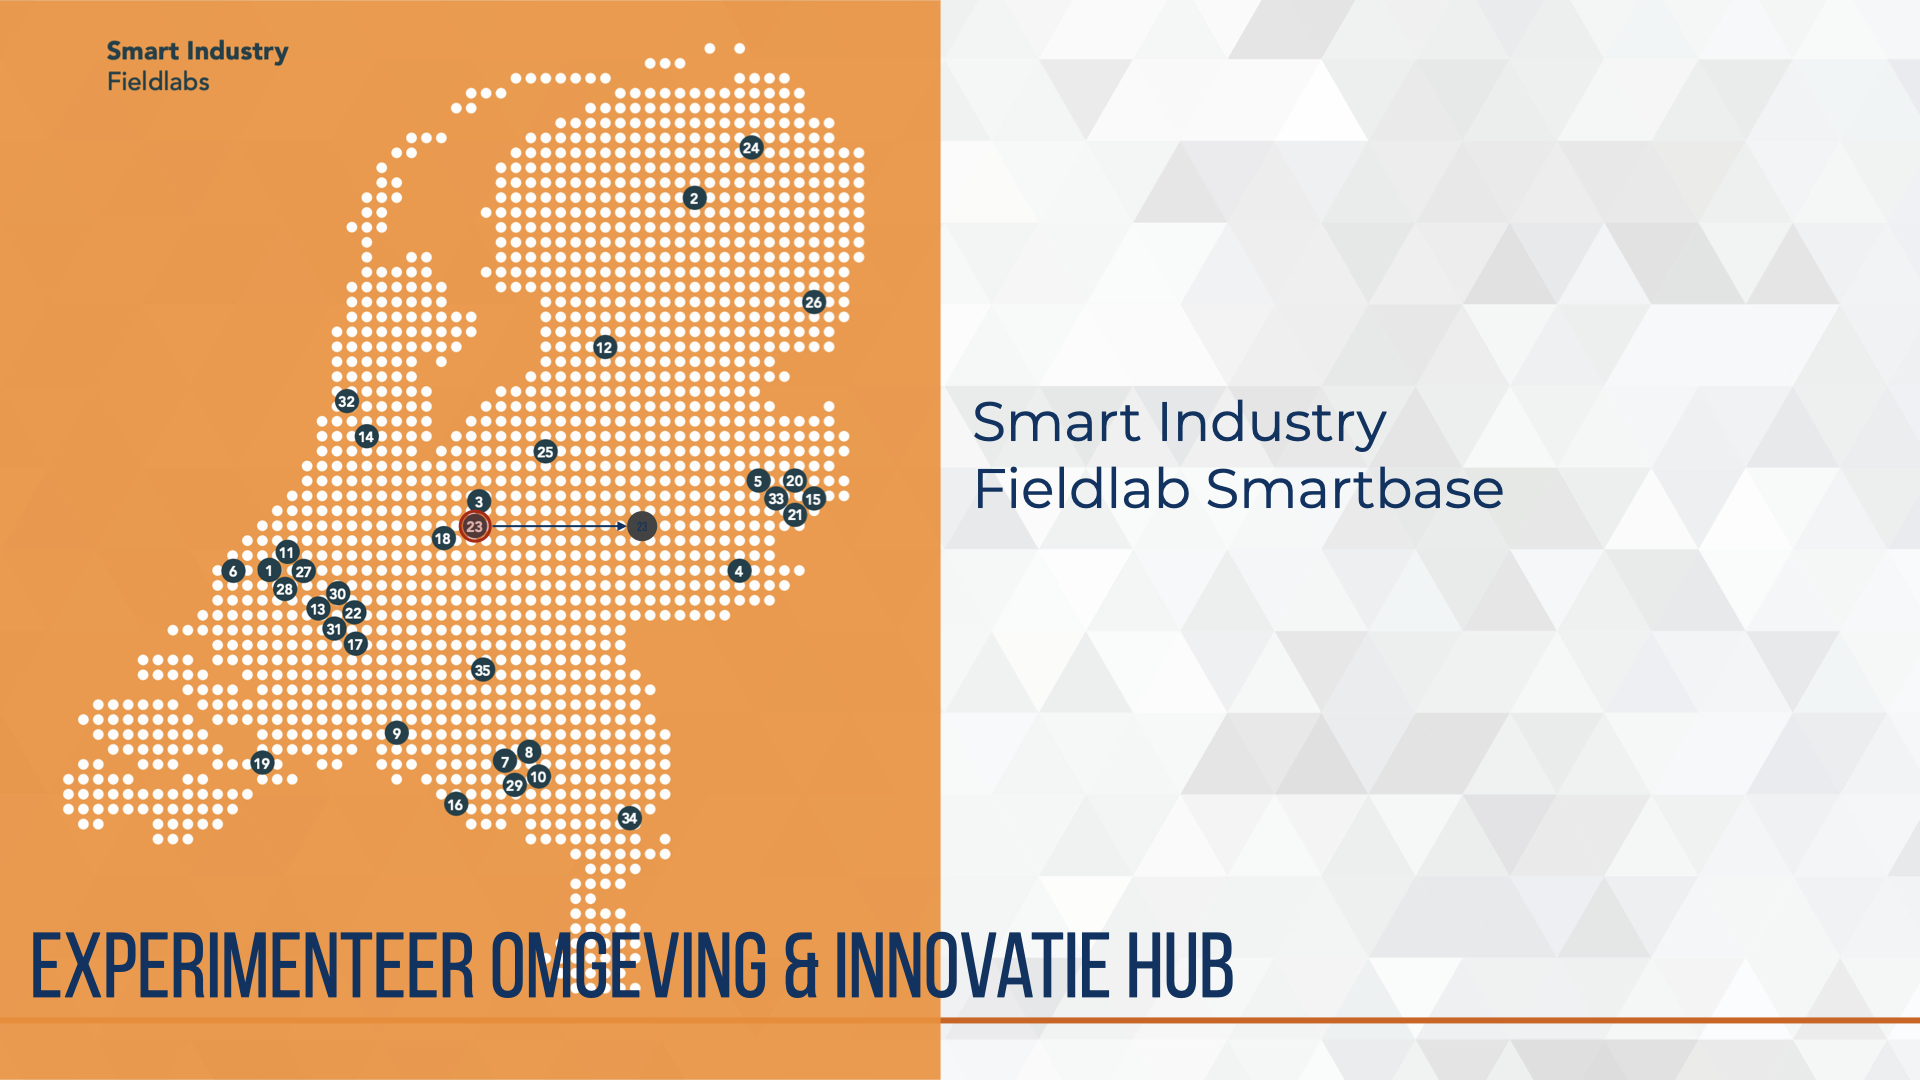
\includegraphics[width=26.67in]{data/keynote-slides/20200430-CDE-Designprocess/20200430-CDE-Designprocess.009-6} \caption{Fieldlabs van Smart industry in Nederland }\label{fig:unnamed-chunk-11}
\end{figure}

De eerste grootschalige uitvraag aan de markt heeft in 2016 plaats gevonden. Gericht op de base van de toekomst zijn de uitdagingen geschetst op de thema's energie, bescherming, water en logistiek. Op Kamp Soesterberg is de basis van een militair kampement opgebouwd met de formele fieldlab status van Smart Industry. Dit Fieldlab Smartbase heeft de Landmacht veel ervaring en kennis opgeleverd over proces en inhoud.

Sinds september 2019 is het Fieldlab Smartbase verhuist naar Complex Ede-Driesprong waar externe partners kunnen experimenteren binnen de militaire context.

\hypertarget{incubatiehub}{%
\subsubsection{incubatiehub}\label{incubatiehub}}

De Landmacht participeert in verschillende challenges om studenten en start-ups mee te laten denken met onze innovatie vraagstukken. De TU Challenges is daarvan een voorbeeld. Wij hopen op termijn te werken aan incubatiehubs waar verschillende partners samen werken aan innovatie vraagstukken waaronder die van de Landmacht.

\hypertarget{kort-cyclisch-moderniseren}{%
\chapter{How to think}\label{kort-cyclisch-moderniseren}}

De landmacht is een overheids organisatie die -waar nodig- een zwaardmacht moet zijn op plekken waar vrede en veiligheid geen vanzelfsprekendheid is. Vanuit de grondwettelijke taken is afgeleid hoe de Landmacht optreedt, welke materieel en personele middelen daarvoor nodig zijn en hoe dit wordt georganiseerd. Deze lineaire denkmodellen dragen decenia lang bij aan de innovatie in het landoptreden. De bestaande Landmacht organisatie is in een continue verbeter modus vanuit deze volgordelijkheid.

De technologische en sociale innovaties gaan echter zo snel dat ook op andere, snellere manieren moet worden gekeken naar modernisering van de bestaande organisatie en vernieuwing voor de toekomstige organisatie.

Military Design \& Innovation geeft manieren om innovatie bij de Landmacht uit te voeren in het tempo van de markt. Centraal staat daarbij een integrale aanpak, met externe partijen door experimenten. Het denkmodel wat we hierbij gebruiken heet `de effectbrenger.'

\hypertarget{effectbrenger}{%
\section{effectbrenger}\label{effectbrenger}}

\begin{figure}
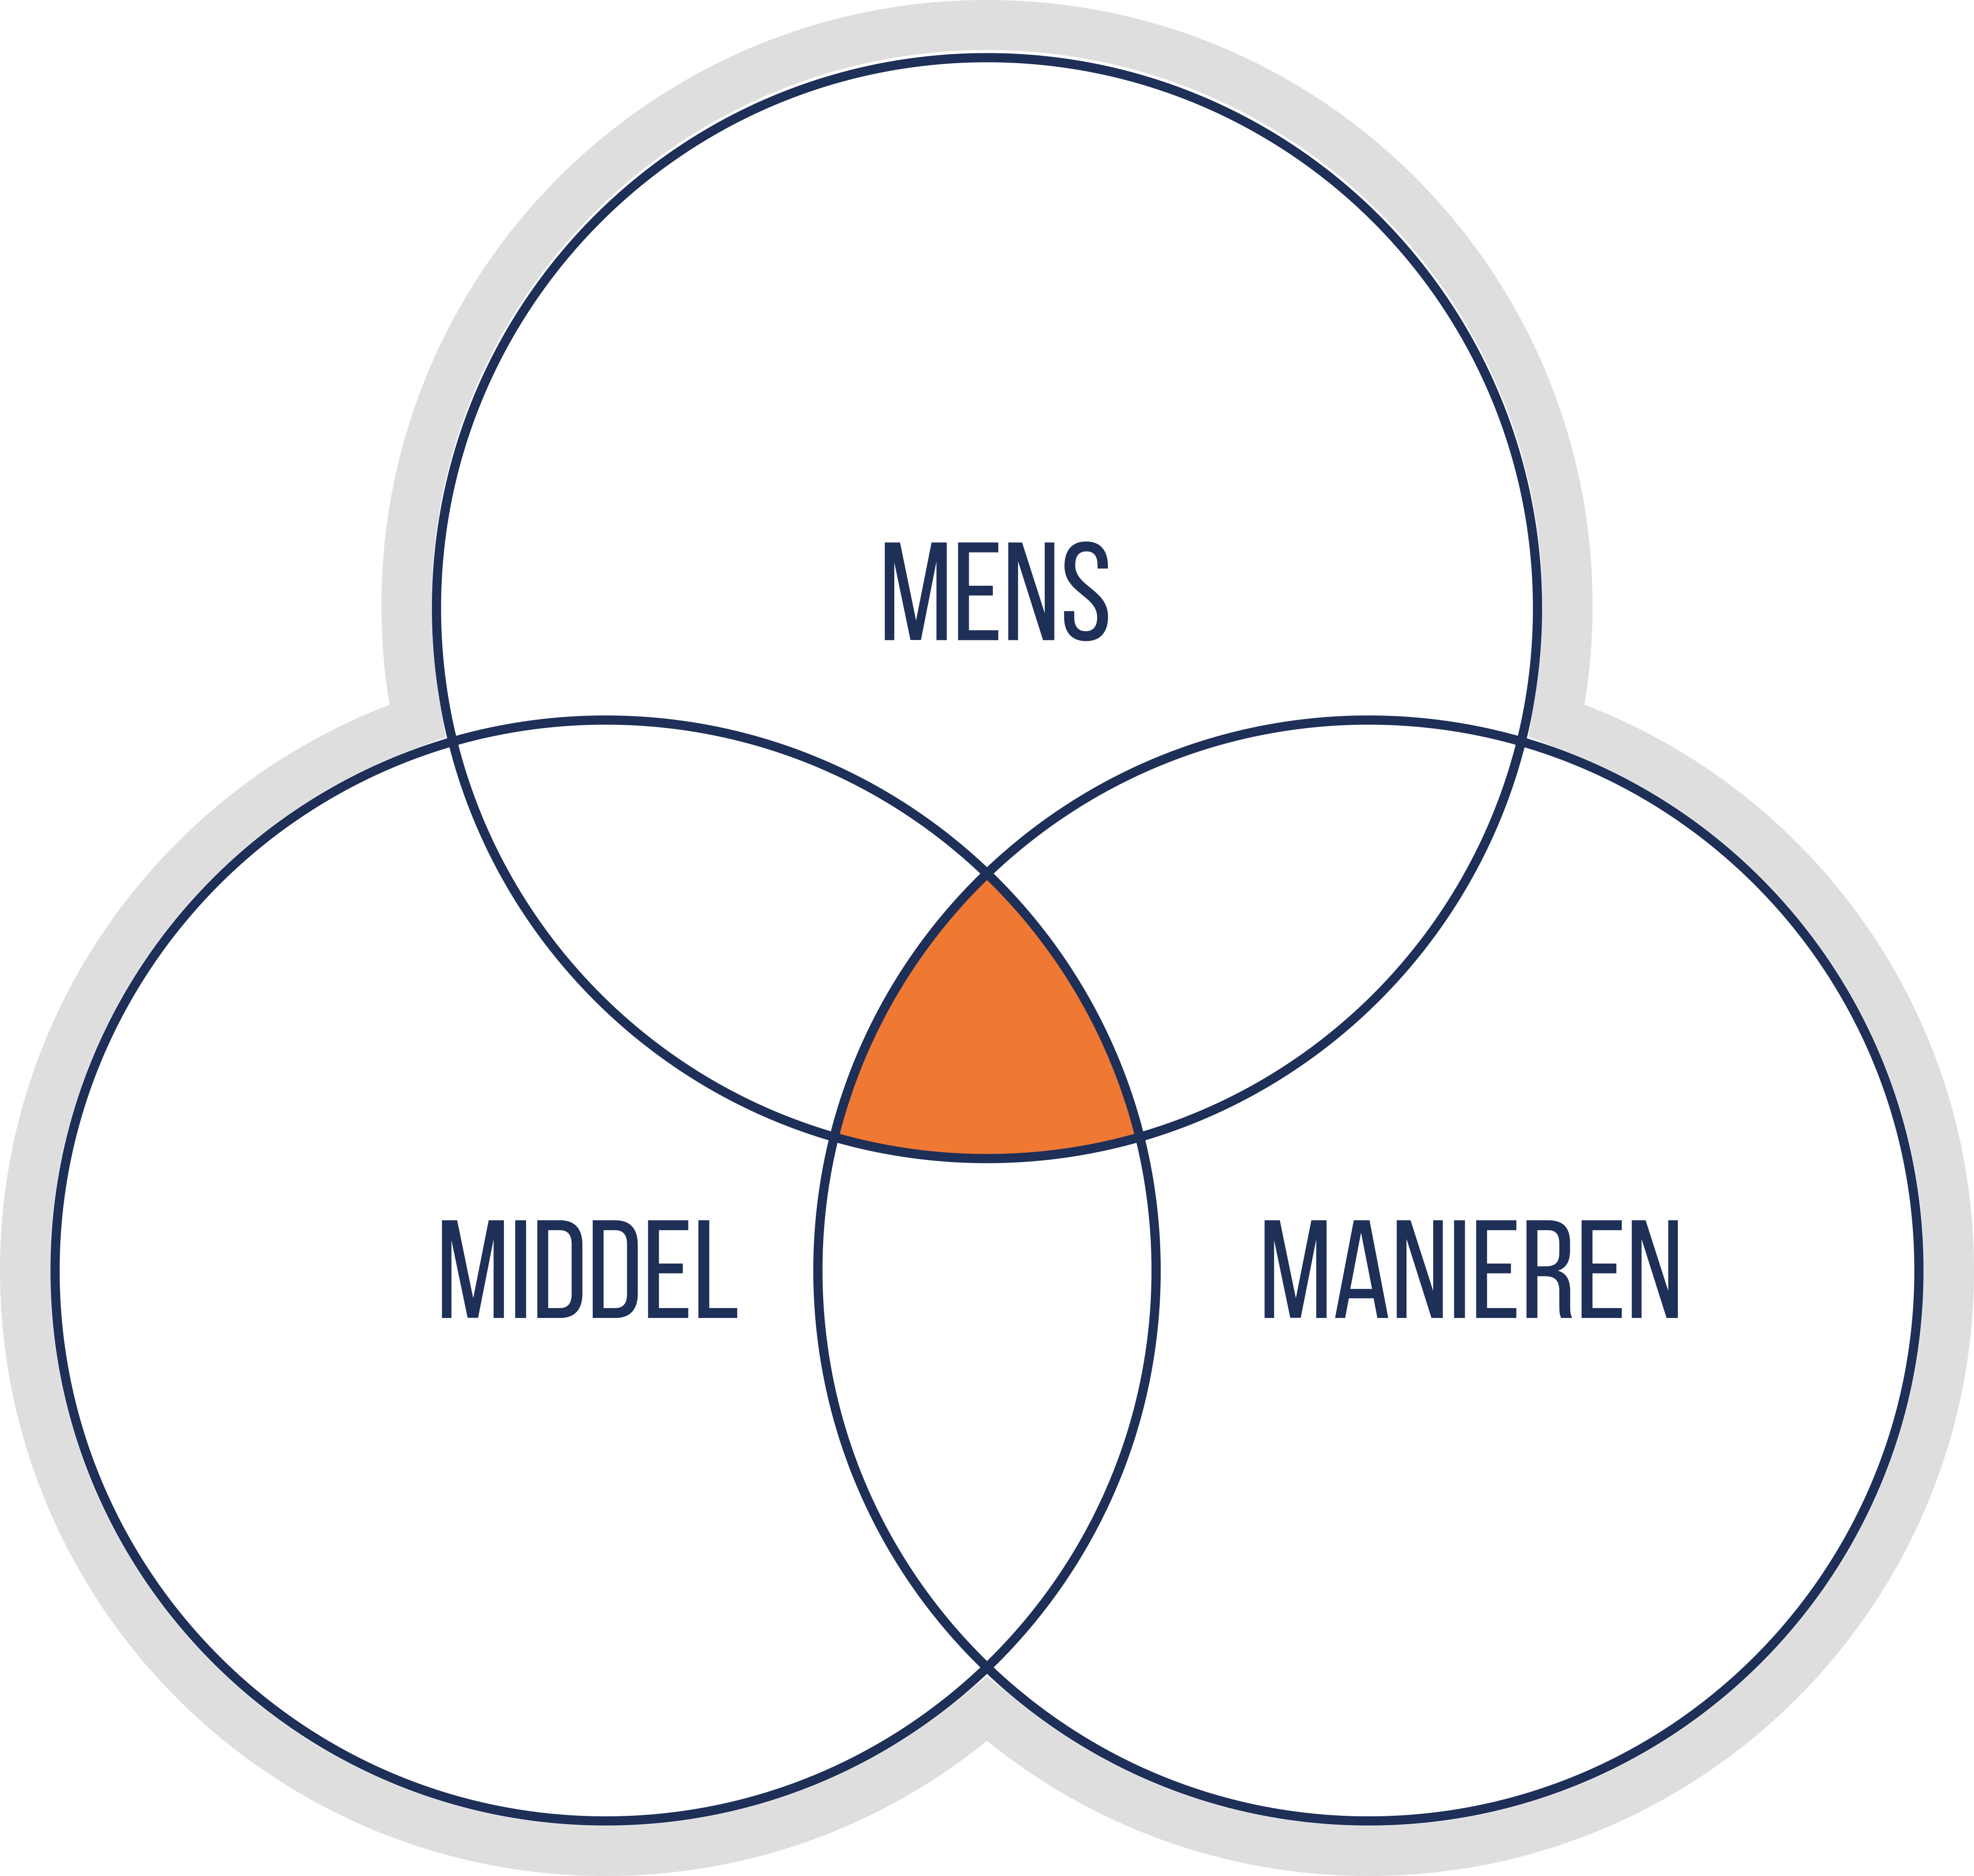
\includegraphics[width=350pt]{data/images/20210324-MDI-mmm-model} \caption{De unieke combinatie van mens, manier en middel maakt een effectbrenger.}\label{fig:mmm-model}
\end{figure}

Een military capability, organisatie onderdeel of subsysteem is een unieke combinatie van mens, manieren en middel(en). Deze unieke combinatie noemen we een effectbrenger.

\begin{figure}
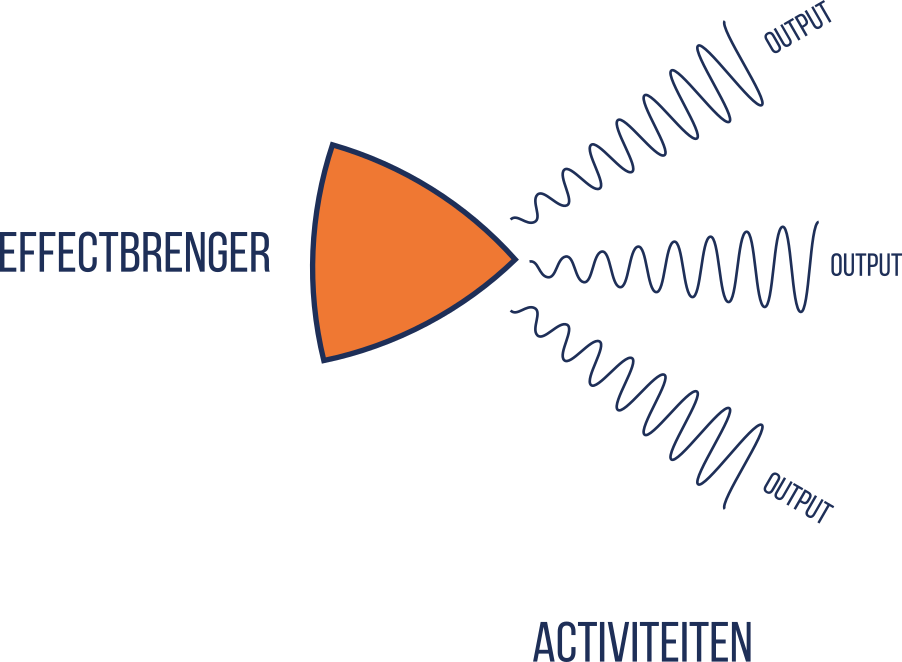
\includegraphics[width=400pt]{data/images/20210324-MDI-effectbrenger} \caption{Een effectbrenger genereert activiteiten met een specifieke output.}\label{fig:effectbrenger}
\end{figure}

Deze effectbrenger voert activiteiten uit met een specifieke, direct te relateren, output. Dit geheel van effectbrenger, activiteiten en output is een zelfstandig en gesloten systeem. De output is afhankelijk van de effectbrenger en activiteiten.

\begin{figure}
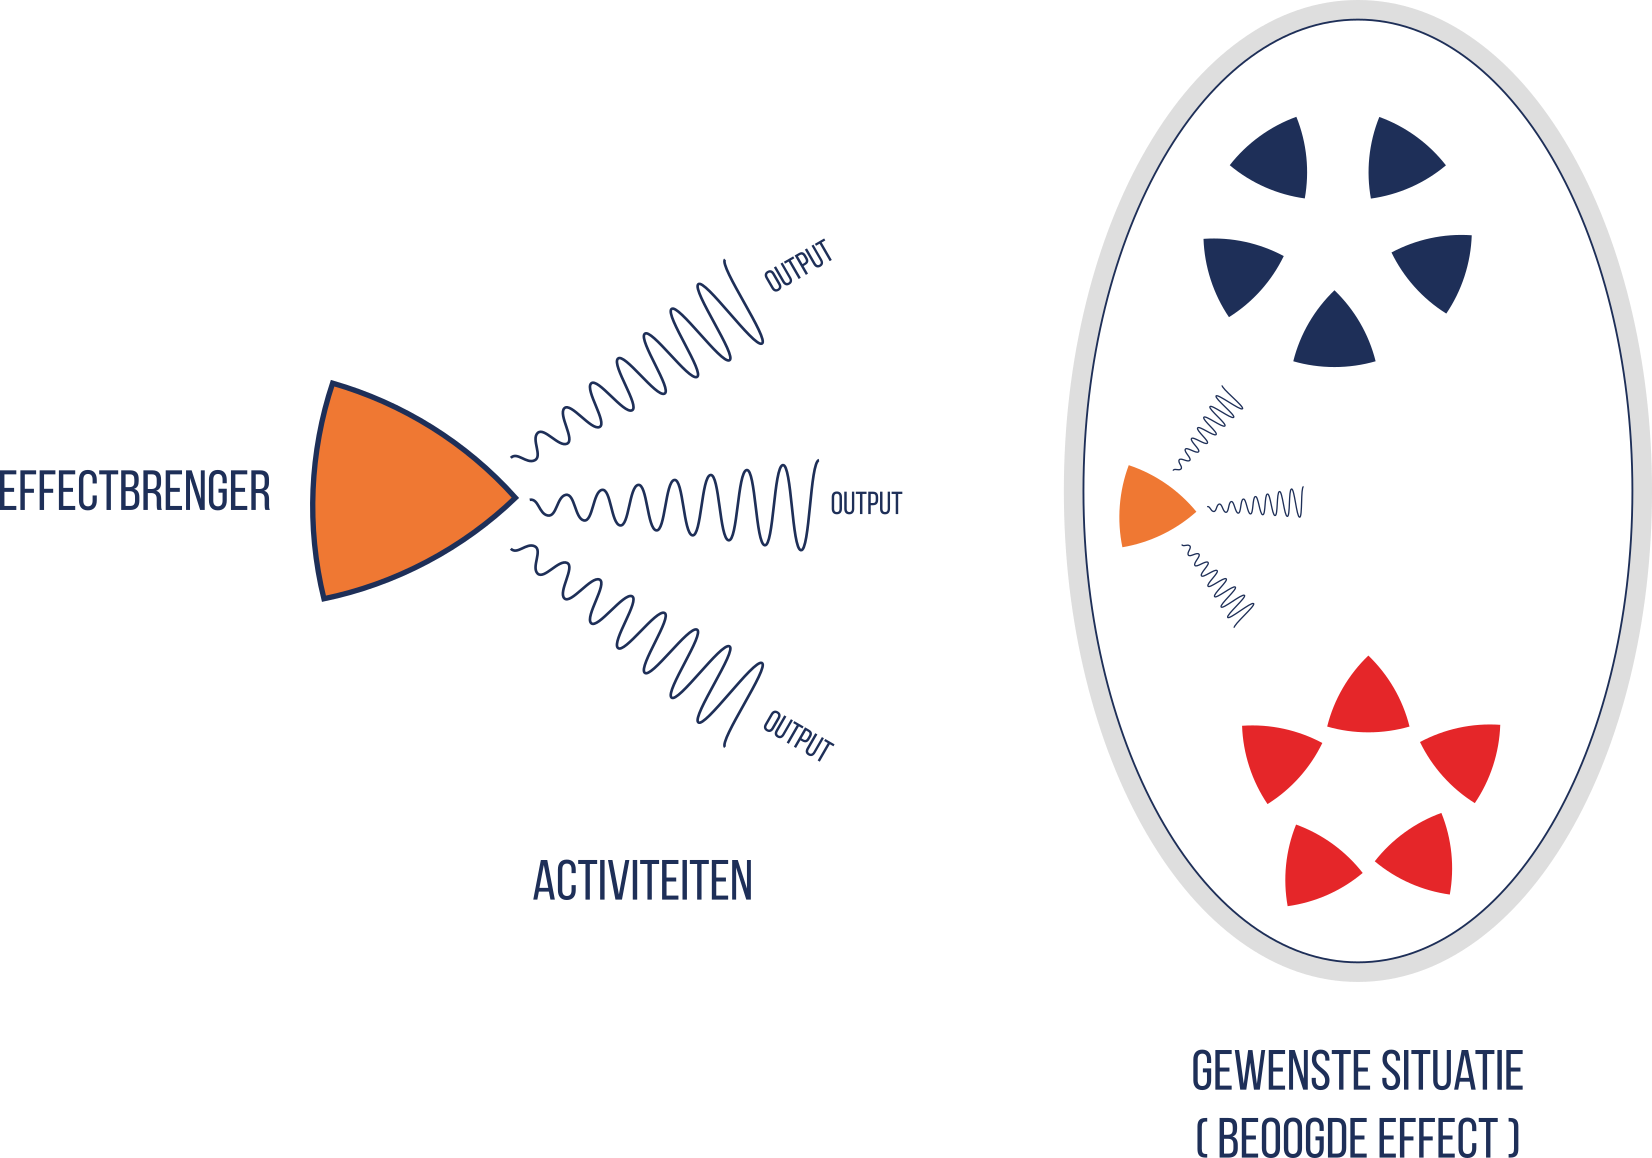
\includegraphics[width=450pt]{data/images/20210324-MDI-effectbrenger-ei} \caption{In een specifieke context creëert een effectbrenger met acitiviteiten en output een effect vanuit de omgeving.}\label{fig:effectbrenger-met-ei}
\end{figure}

\hypertarget{effect}{%
\section{effect}\label{effect}}

De activiteiten en output genereren een reactie in de omgeving, het indirect te relateren, effect. Dit creëert de waarde en impact van de effectbrenger in een specifieke context.

\begin{figure}
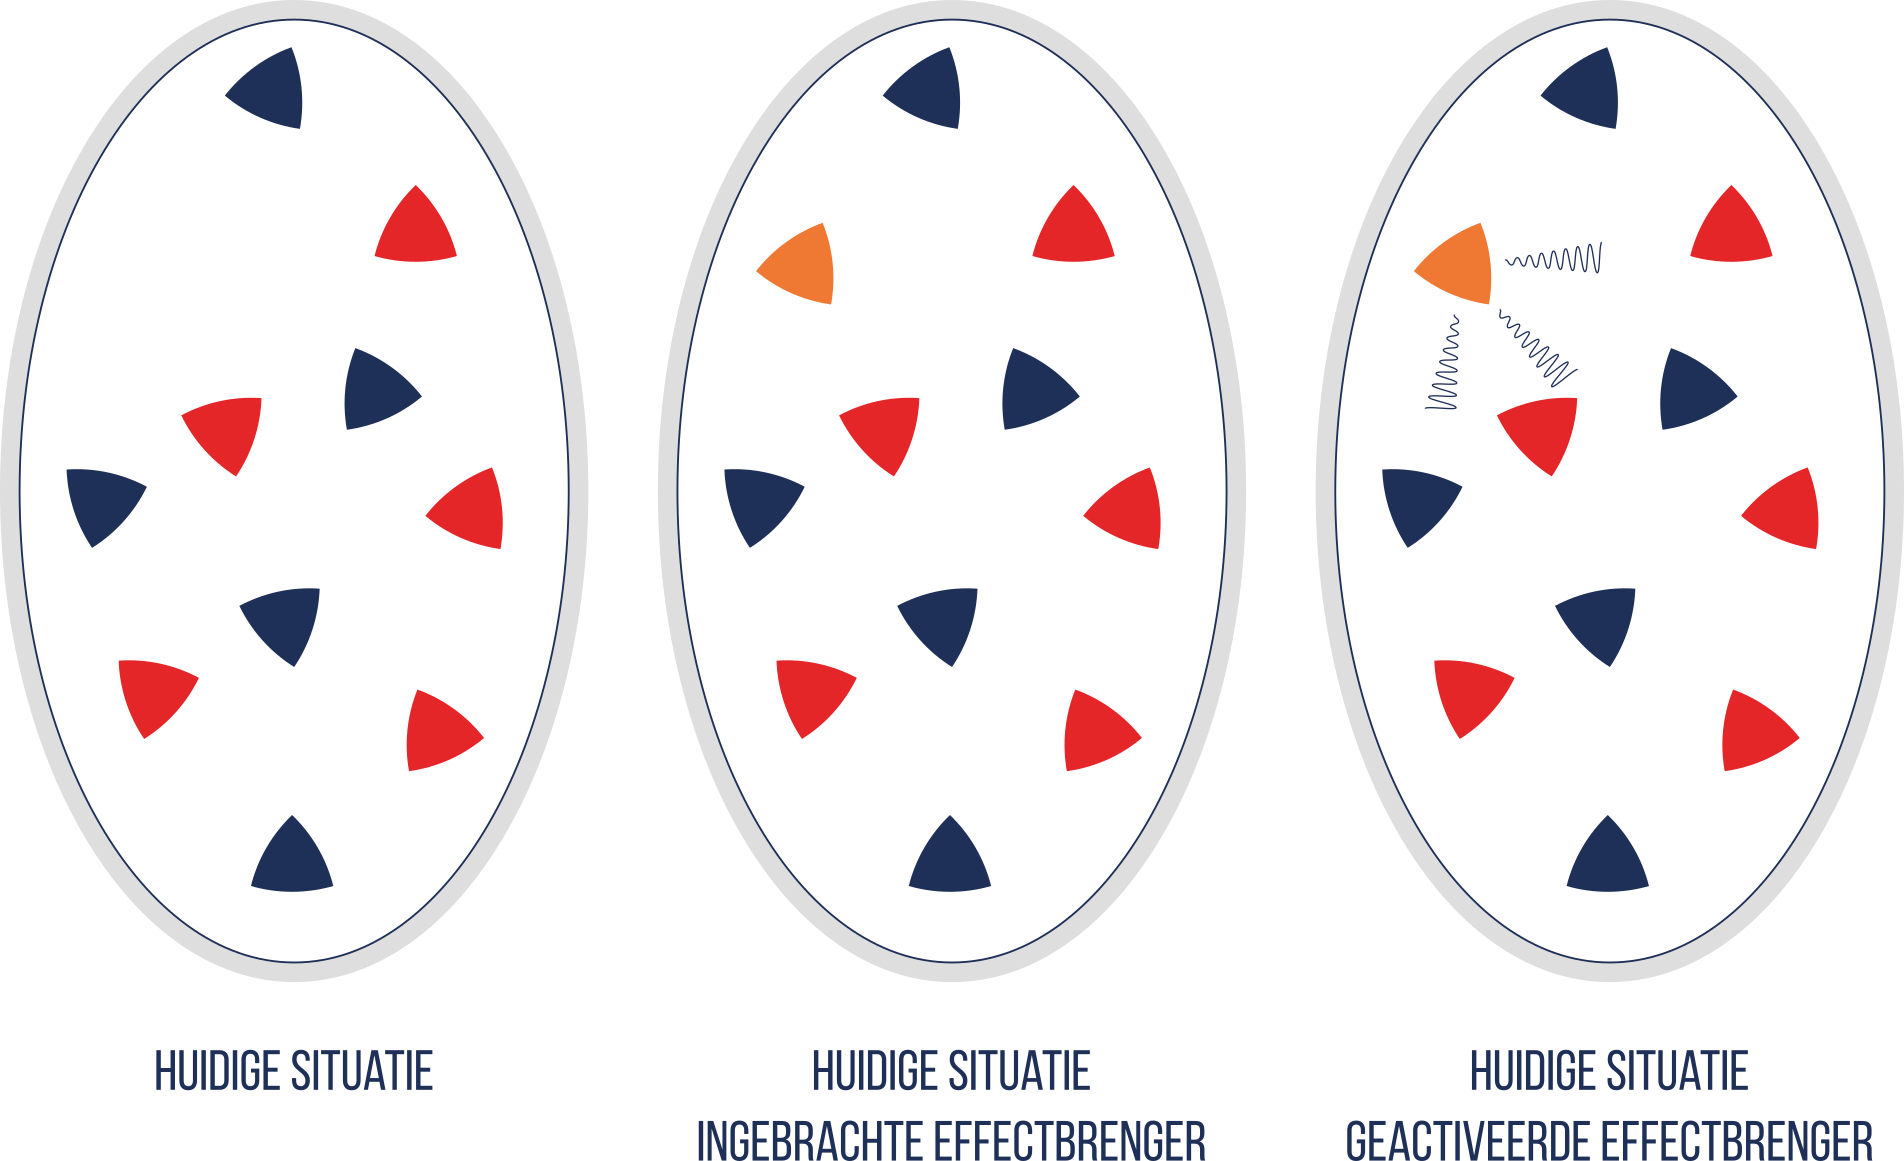
\includegraphics[width=550pt]{data/images/20210324-MDI-eieren-huidig} \caption{Abstracte vormgeving van een specifieke context met een ingebrachte en geactiveerde effectbrenger.}\label{fig:effectbrenger-in-eieren}
\end{figure}

Het feit dat de context veranderd bij het inbrengen of activeren van een effectbrenger is geen causaliteit maar hoogstens een correlatie. Gedegen experimenteren en valideren is daarom van belang.

\hypertarget{context}{%
\section{context}\label{context}}

In de beschrijving van de paragraaf \ref{effect} effecten werd een eerste relatie gelegd met een context. In deze paragraaf \ref{context} worden de soorten context beschreven die regelmatig terugkomen binnen Military Design \& Innovation. Allereerst een kleine `side step' over de betekenis van context.

Oxford Dictionary spreekt over ``The circumstances that form the setting for an event, statement, or idea, and in terms of which it can be fully understood.''"(\protect\hyperlink{ref-context}{{``Context,''} n.d.}) en het Van Dale woordenboek definieert context als `samenhang.' De beschrijving die Military Design \& Innovation --voorlopig-- aanhoudt is:

\begin{quote}
``de plaats- en tijdsgebonden setting van samenhangende relevante actoren en factoren van invloed rondom een specifieke effectbrenger, bezien vanuit verschillende standpunten, perspectieven en percepties.''
\end{quote}

De context is daarmee beschrijvend en geeft betekenis aan de opgaaf, eenheid en effectbrenger. Bij het innoveren, moderniseren en transformeren binnen de Koninklijke Landmacht is de setting gedefinieerd als `het landoptreden,' zodat de inspanningen gericht blijven op de operationele taak. We onderscheiden hierin de probleem, experimentele en toekomstige context.

Actoren en factoren die nodig zijn voor een innovatie worden binnen Military Design \& Innovation gezien als randvoorwaardelijke mensen, manieren en middelen voor het organiseren en realiseren van innovatie.

\hypertarget{probleem-context}{%
\subsection{probleem context}\label{probleem-context}}

\begin{figure}
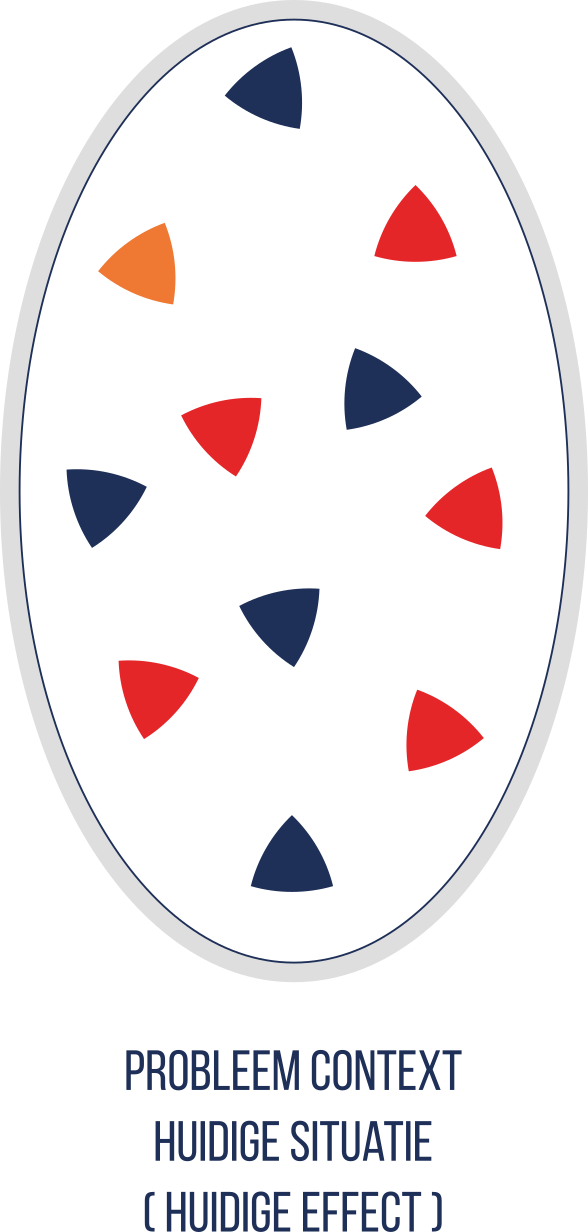
\includegraphics[width=150pt]{data/images/20210324-MDI-eieren-beweging-1} \caption{Abstracte vormgeving van probleem context.}\label{fig:eieren-in-beweging-1}
\end{figure}

Door het opzetten van een probleem context krijgen de betrokken actoren een gemeenschappelijk beeld van de operationele militaire setting waarop het innovatie vraagstuk gericht is.

In een probleem context beschouwen we een voorgestelde --vernieuwde-- effectbrenger en beschrijven we de huidige operationele setting van een eenheid. Meestal is sprake van een bestaande effectbrenger die verbeterd wordt, soms wordt een geheel nieuwe effectbrenger ontwikkeld.

Potentiële partners plaatsen de opgaaf in militair operationele setting. Voor militairen is deze setting `normaal' omdat het hun vakgebied en realiteit is maar voor een niet-militair kan het bijzonder, soms `ver van het bed' en vaak slecht inleefbaar zijn. Dit betekend ook dat militairen blinde vlekken hebben voor de setting en niet-militaire nieuwe inzichten geven. Gezamenlijk werken aan de probleem contrext verijkt daarmee de vraagarticulatie en aanbodspecificatie.

\hypertarget{experimentele-context}{%
\subsection{experimentele context}\label{experimentele-context}}

\begin{figure}
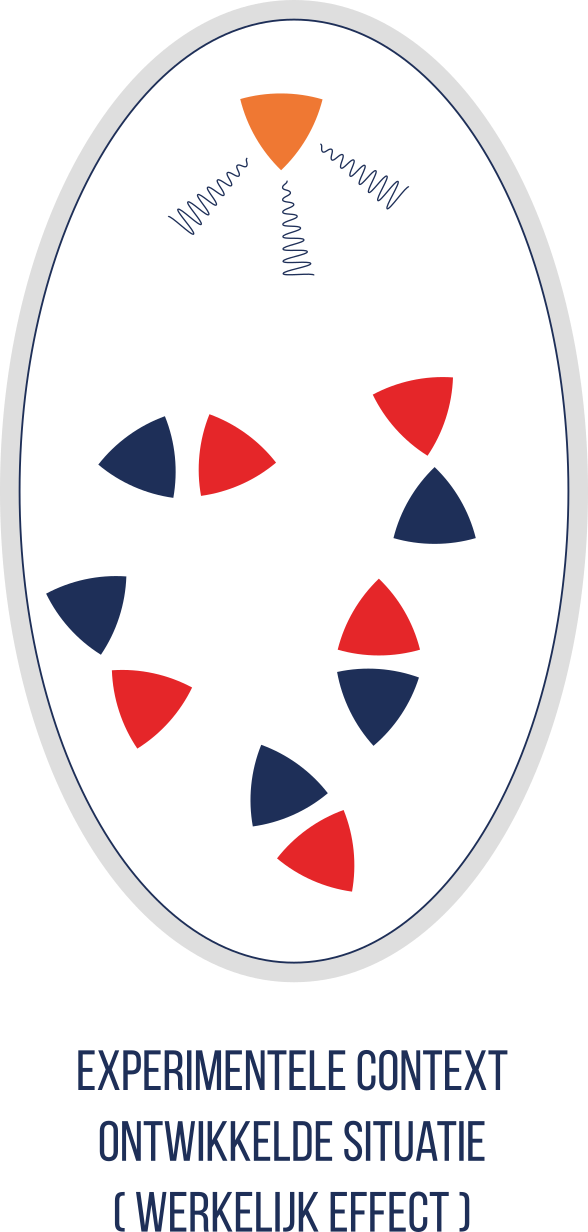
\includegraphics[width=150pt]{data/images/20210324-MDI-eieren-beweging-2} \caption{Abstracte vormgeving van experimentele context.}\label{fig:eieren-in-beweging-2}
\end{figure}

Door het opzetten van een experimentele context kan de ontwikkelde effectbrenger worden beproefd en kunnen de werkelijke reacties van de omgeving worden waargenomen.

Militaire experimenten vinden zelden plaats in een laboratorium of operationele realiteit. Toch is een gecontroleerde omgeving noodzakelijk voor het meten en valideren van ontwikkelde effectbrengers. De mate van controle is mede afhankelijk van het technical readiness level (TRL) van middelen, de maturiteit van de effectbrenger en vigerende wet- en regelgeving. Ook de wijze van meten en valideren beinvloed de gewenste setting van het experiment.

Omdat we het traject zoveel mogelijk in samenhang doorlopen en tempo willen behouden, starten we zo vroeg mogelijk met het opzetten en vaststellen van de expermentele context. Samen met interne en externe partners, het kenniscentrum creëeren we een gecontroleerde operationele omgeving met een eenheid in training, oefening of bij inzet.

\hypertarget{toekomstige-context}{%
\subsection{toekomstige context}\label{toekomstige-context}}

\begin{figure}
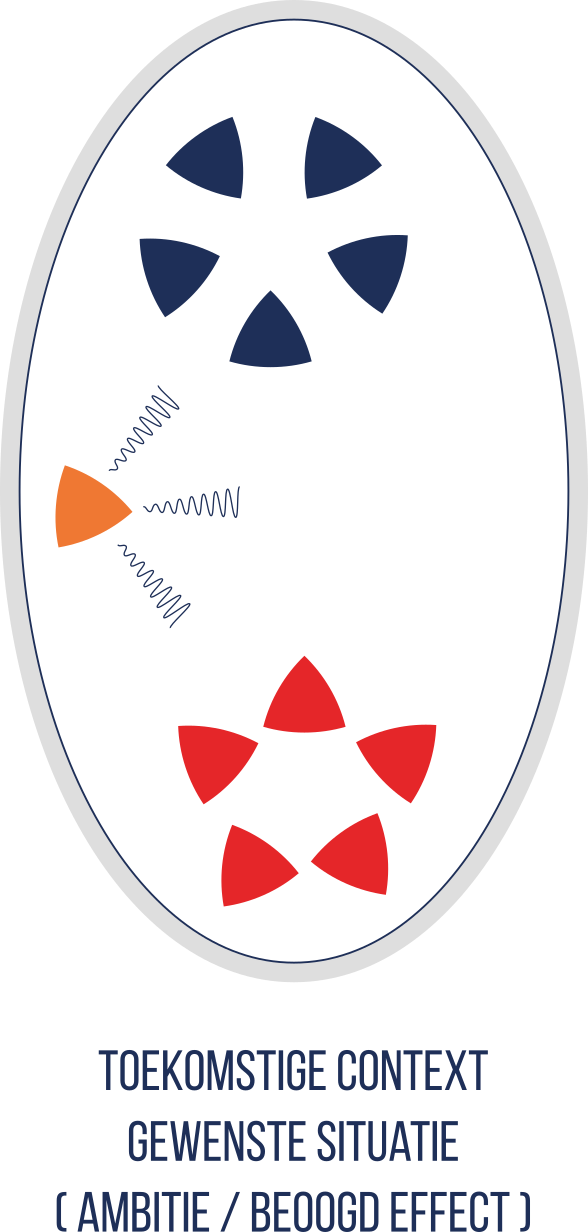
\includegraphics[width=150pt]{data/images/20210324-MDI-eieren-beweging-3} \caption{Abstracte vormgeving van toekomstige context.}\label{fig:eieren-in-beweging-3}
\end{figure}

Het Ministerie Defensie schetste toekomstscenario's en formuleerde ambities en inrichtingsprincipes. De Koninklijke Landmacht beschreef een visie en ontwikkellijnen. Het is aan kennisadviseurs, kenniswerkers en subject matter experts om daarbinnen ambities, operationele wensen en behoeften, technologische ontwikkelingen en inventies te programmeren.

Dit bereiken we door samen met relevante actoren te werken aan een gemeenschappelijk beeld van de toekomstige setting waarin militaire capaciteiten optreden. Daarin worden ook de gewenste effecten gedefinieerd die het optreden moeten creëeren. De setting met de gewenste effecten maakt de toekomstige context.

Door de toekomstige context in het denkmodel te plaatsen onstaat inzicht in de de ontwikkelrichting en meerwaarde van de beoogde effectbrenger. Dit inzicht draagt bij aan designkeuzes en indicatoren voor validatie.

\hypertarget{cde-design-model}{%
\chapter{How to act}\label{cde-design-model}}

Dit hoofdstuk beschrijft een aantal veel gebruikte en doorontwikkelde handelingsperspectieven om gezamenlijk een idee of ambitie te verwezenlijken. Inspiratie voor deze handelingsperspectieven komen van verschillende vakgebieden zoals netwerk- en ketenregie, design-research, aliantiekunde, militaire doctrines, innovatiekunde, engineering, natuurkunde, en militaire inlichtingen. De handelingsperspectieven zijn verwerkt tot technieken en tools van de craftman en beschreven in dit hoofdstuk.

In het aanpakken van een innovatie vraagstuk beschouwen wij deze als een ongetemd probleem in een complexe context. De eerste paragraaf \ref{inleiding-in-wicked-problems} geeft een korte inleiding en achtergrond bij dit soort problemen. De daarop volgende paragrafen beschrijven het frame \ref{framework}, de activiteiten, tools \ref{activiteiten-pallet} en technieken \ref{regisseren} van de crafstman. Kortweg geeft het richting hoe we handelen, wat we doen en in welke volgorde werken we aan het voorliggend vraagstuk.

\hypertarget{inleiding-in-wicked-problems}{%
\section{inleiding in wicked problems}\label{inleiding-in-wicked-problems}}

\begin{quote}
DISCLAIMER: Het belang om dit onderwerp op te nemen kwam tijdens het schrijven van de eerste versie naar voren. Deze paragraaf \ref{inleiding-in-wicked-problems} is nog niet herschreven naar de laatste inzichten maar komen voort uit speaker notes van verschillende presentaties.
\end{quote}

\hypertarget{ongetemde-problemen}{%
\subsection{ongetemde problemen}\label{ongetemde-problemen}}

Wanneer potentiele samenwerkende partners verschillende oorzaken of invalshoeken zien voor een probleem spreken we van een ongetemd probleem of `wicked-problem.' Deze ongetemde problemen komen voor in alle lagen, sectoren en gebieden van organisaties en maatschappijen. Ongetemde problemen zijn niet zomaar opgelost en kennen geen afzonderlijke probleemeigenaar of centrale verantwoordelijke. Het `vacuüm' van centrale verantwoordelijke wordt steeds vaker opgevuld door een alliantie van diverse organisaties. Deze allianties zijn van tijdelijke aard en hebben een horinzontale machtsrelatie. In de praktijk creëren deze allianties verrassende oplossingen voor ongetemde problemen.

\hypertarget{aanpak-ongetemde-problemen}{%
\subsection{aanpak ongetemde problemen}\label{aanpak-ongetemde-problemen}}

Er is geen pasklaar antwoord of eenduidig proces om ongetemde problemen met een alliantie aan te pakken. Wel bestaan er succesvolle voorbeelden met terugkerende activiteiten. De Military Design \& Innovation aanpak is deels geinspireerd door voorbeelden van innovatieve cooperaties en gemeentelijke- en provinciale overheden.

Een aanpak begint met het exploreren van de context en actoren, centraal stellen van (organisatorische) behoeften, belangen, waarden en plichten, en het organiseren in netwerken of ketens. Vervolgens leren de relevante partijen door samen te werken aan oplossingsrichtingen en deze met experimente in de praktijk te brengen. Deze aanpak van exploreren, articuleren en experimenteren passen we toe in Military Design \& Innovation.

\hypertarget{aanpak-in-militaire-context}{%
\subsection{aanpak in militaire context}\label{aanpak-in-militaire-context}}

Bij het exploreren van het vraagstuk en de actoren bevinden we ons op onbekend terrein. Aan de hand van succes-indicatoren, canvassen en ambities brengen we in werksessies de context, bestaande initiatieven en stakeholders in kaart, zoals een ontdekkingsreiziger een kaart intekent en daarbij navigeert op bekende referentiepunten met kompas en sextant.

Het resultaat zijn een gearticuleerd probleem, probleemcontext en vraag waarmee potentiele partijen worden benaderd. Partijen willen deelnemen vanwege hun belangen, waarden, interesse of machtspositie en worden geselecteerd als zij een effectieve bijdrage kunnen leveren aan de oplossing(srichting). Afhankelijk van de abstracte of concrete beschrijving van het vraagstuk vinden meerdere iteraties plaats om de vragen en mogelijke oplossingen helder te krijgen.

Een consistente vraagarticulatie slaat een brug tussen de probleem context en ambitie, opdrachtgever en -nemer en idee en implementatie. Het militairy design framework ondersteund de samenwerkende partijen bij het creëren van een consistent geframde en gearticuleerde vraag.

\hypertarget{framework}{%
\section{framework}\label{framework}}

Het framework biedt houvast voor het ontwerpen, ontwikkelen \& experimenteren en samenwerken aan gemoderniseerde effectbrengers in specifieke situaties. De betrokken vakmensen creëeren inzicht en overzicht op hun handelingsperspectieven in een traject. Het military design framework modeleert in één figuur (\ref{fig:design-model}) de ontwikkeling van een effectbrenger, oftewel het traject van idee tot en met valideren, in een abstracte visualisatie.

\begin{figure}
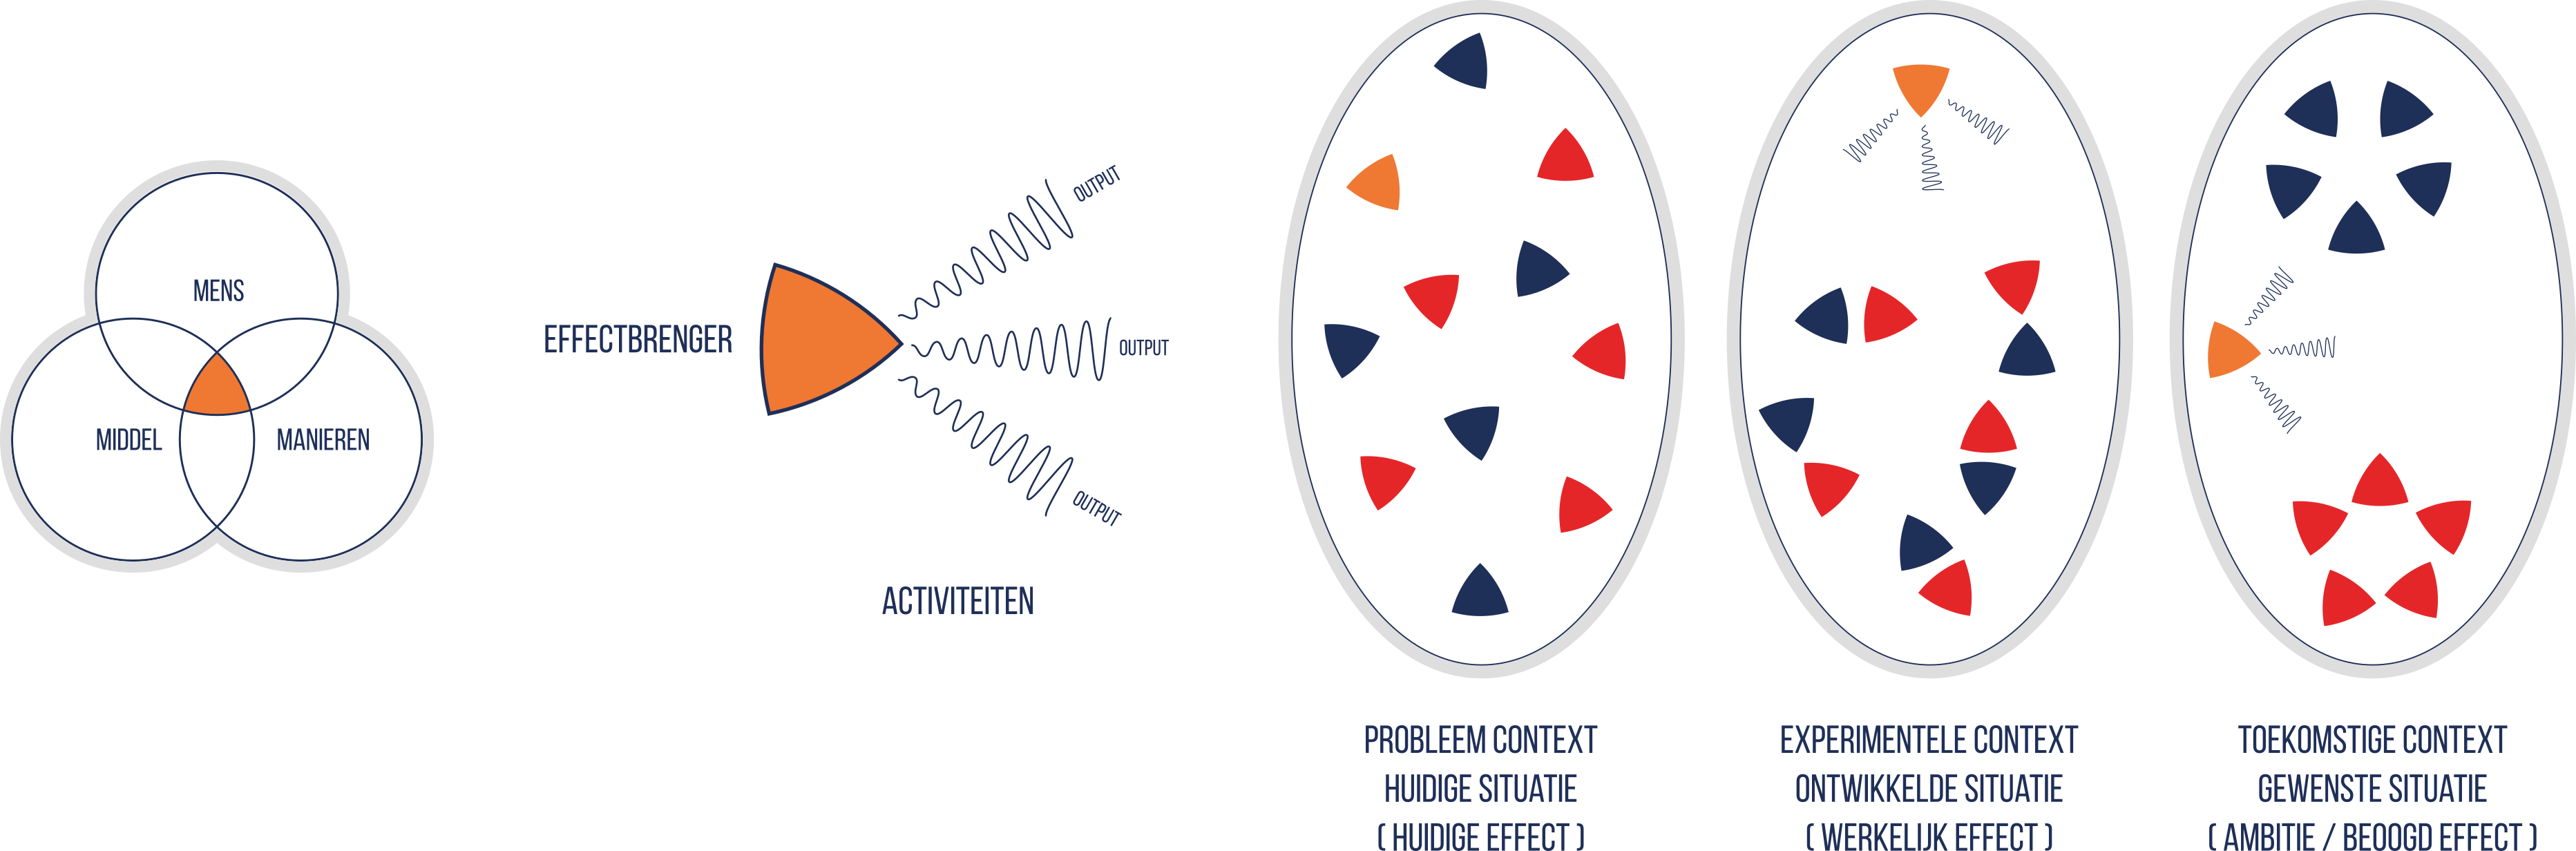
\includegraphics[width=51.79in]{data/images/20210324-MDI-design-model} \caption{Military Design framework.}\label{fig:design-model}
\end{figure}

Gezamenlijk wordt inzicht gecreerd in de mogelijkheden van de markt voor de --toekomstige-- utidagingen in het landoptreden. Daarin zagen we twee bewegingen, vanuit de toekomstige context (forecasting) of vanuit de huidige context (backcasting). Forecasting gaat van links naar rechts. Dat wil zeggen, door het maken van nieuwe combinaties van mens, manieren en middel ontstaan (ver)nieuwde effectbrengers. Met hun activiteiten dragen zij bij aan vernieuwde effecten in een toekomstige context. Backcasting gaat van rechts naar links. Dat wil zeggen, vanuit ambities en operationele behoeften worden de gewenste effecten, output en activiteit inzichtelijk. Hiermee wordt de beoogde effectbrenger geschetst. Verschillende variaties van de beoogde effectbrenger worden ontwikkeld door het combineren van mensen, manieren en middelen.

In een traject stellen we de hypothese dat een gemoderniseerde effectbrenger bijdraagt aan een gewenst effect in een toekomstige context. Tijdens de experimenten worden gemoderniseerde effectbrengers ingebracht in een afgebakende, gecontroleerde situatie. In deze experimentele context worden de prestaties en effecten gemeten.

\hypertarget{activiteiten-pallet}{%
\section{activiteiten pallet}\label{activiteiten-pallet}}

\begin{figure}
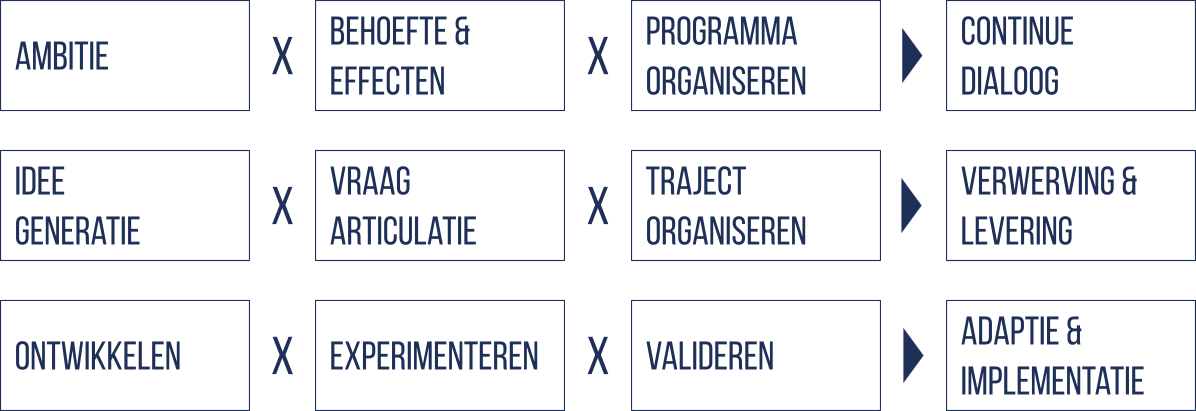
\includegraphics[width=16.61in]{data/images/20210401-MDI-activiteiten-pallet} \caption{Pallet aan activiteiten binnen Military Design \& Innovatie.}\label{fig:unnamed-chunk-17}
\end{figure}

Om ambities en ideëen te brengen naar implementatie moeten veel activiteiten worden ingezet. Omdat we een idee binnen Military Design \& Innovation benaderen als een ongetemd probleem is er geen uitgestippeld pad maar ligt er een ontdekkingstocht in het verschiet. In deze tocht reflecteren we na iedere stap. Wat kunnen de volgende stappen zijn en welke richting moeten deze stappen opgaan?

In deze paragraaf worden de activiteiten van het huidige pallet toegelicht zodat ze worden begrepen. Het doorgronden van de activiteiten vindt plaats in de praktijk. Daarom is praktische uitvoering onder begeleiding belangrijker dan theoretisch bestuderen of werken volgens het boekje.

\hypertarget{idee-generatie}{%
\subsection{idee generatie}\label{idee-generatie}}

\begin{figure}
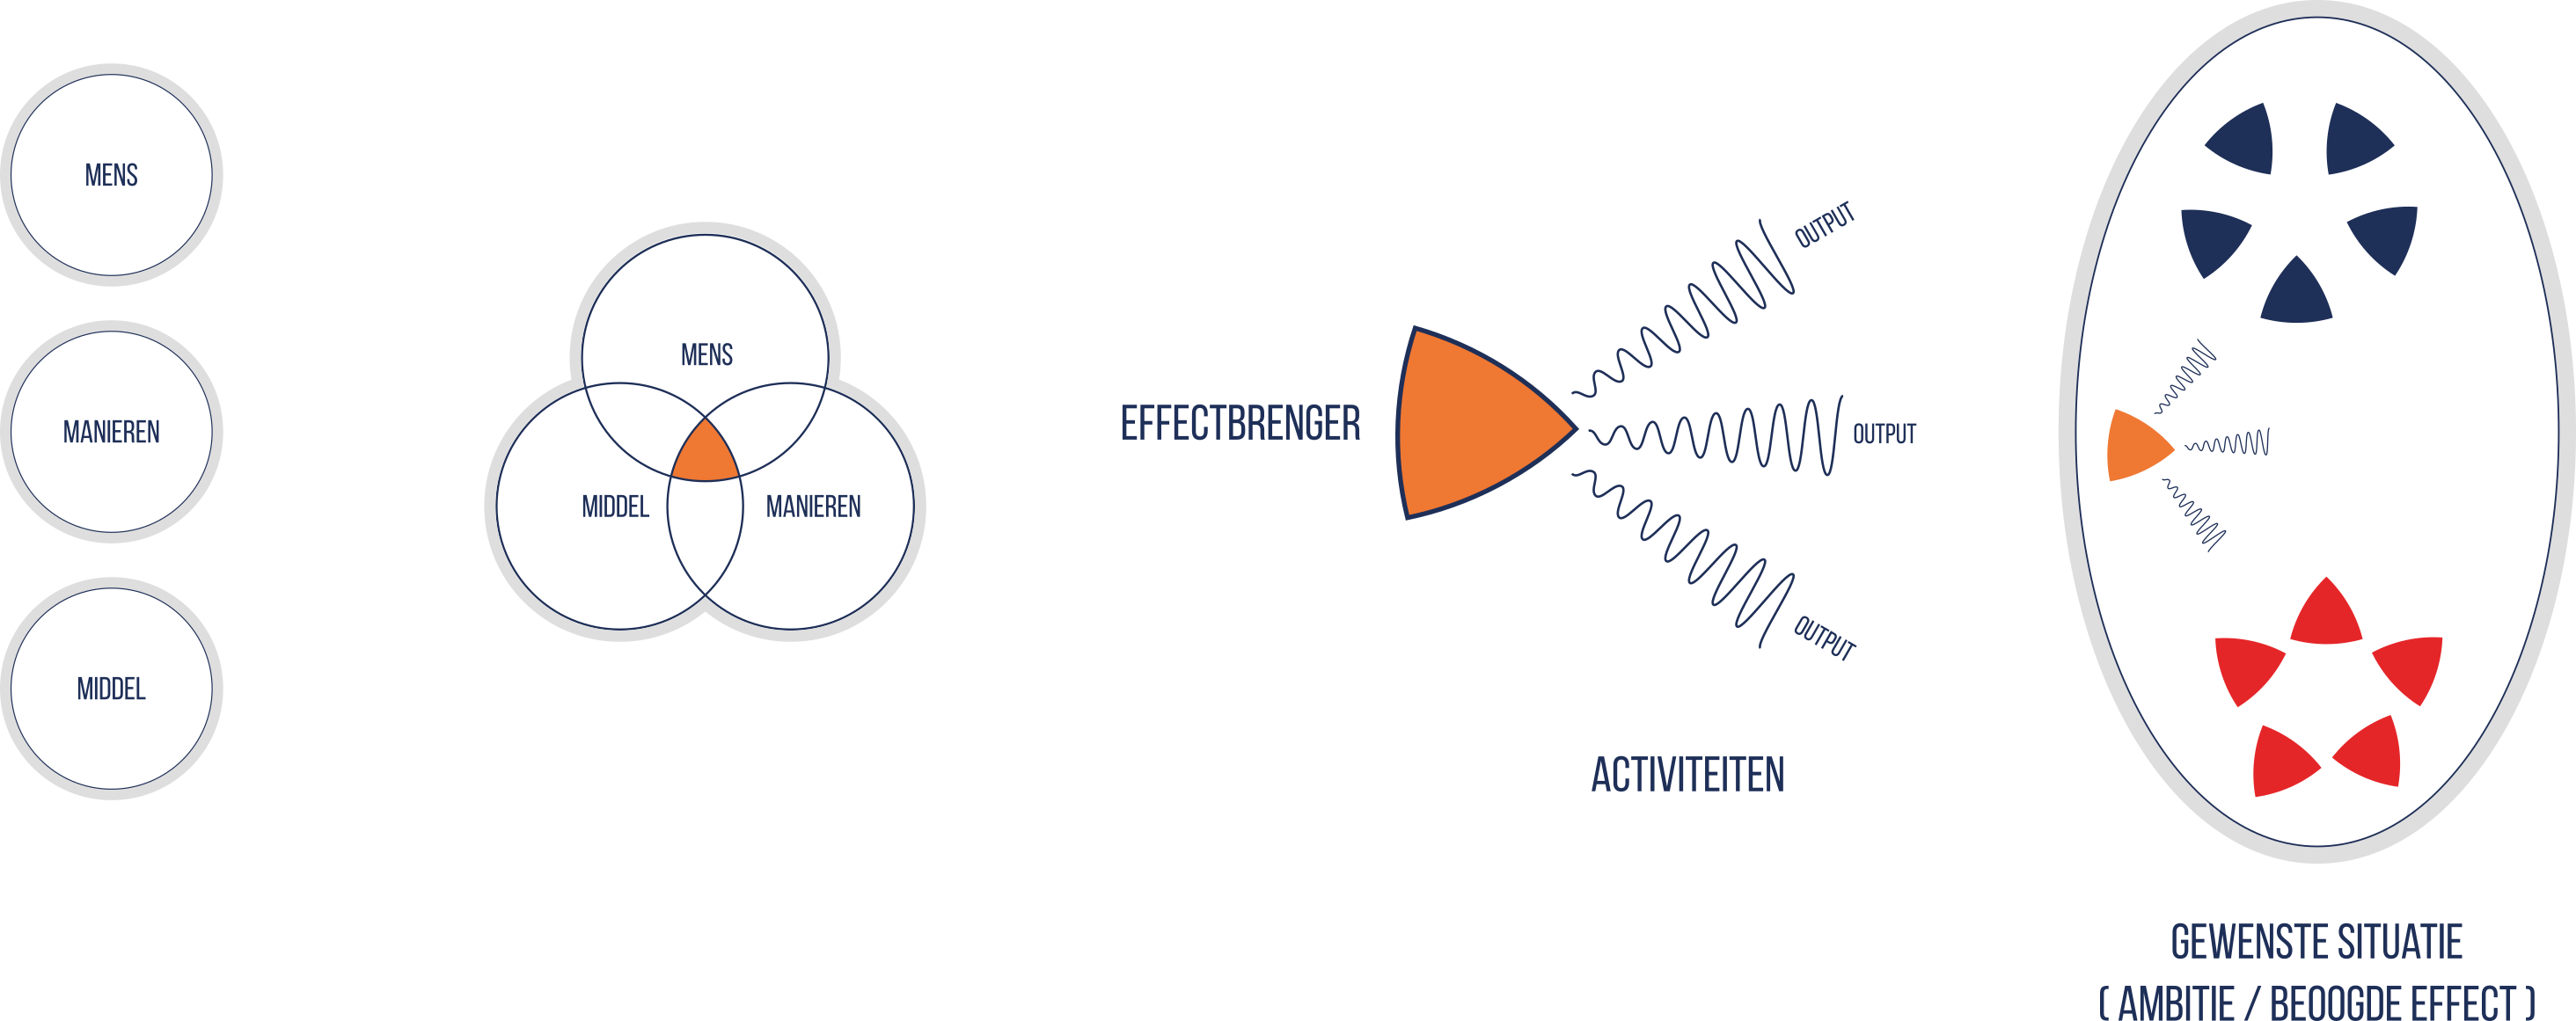
\includegraphics[width=40.67in]{data/images/20210401-MDI-ideegeneratie} \caption{ }\label{fig:unnamed-chunk-18}
\end{figure}

In een forecasting komt een kenniswerker of collega van een parate eenheid met een idee wat een verbetering beloofd op de directe taakstelling, werkomgeving of specifiek vakgebied. Het idee is meestal onvolledig of mist voldoende houvast om direct door te pakken, maar het idee geeft veel informatie over latente vraagstukken, problemen en kansen in een specifieke context. Het is daarom belangrijk om goed te luisteren naar de `binnenlopende ideëen' en deze uit te werken tot een eerste concept. Als ondersteunende tool is hiervoor het canvas `idee generatie 'ontwikkeld. Het stellen van verdiepingsvragen en de 'socratische dialoog' zijn gesprekstechnieken die daarin ondersteunend zijn. De idee-inbrenger beschrijft de beoogde effectbrenger en de toekomstige context kort en bondig zodat dit als idee of design-concept overdraagbaar is.

De centrale deelvragen in deze activiteit zijn:

\begin{enumerate}
\def\labelenumi{\arabic{enumi}.}
\tightlist
\item
  Wat is het idee?
\item
  Wat is er tot nu toe gedaan voor dit idee?
\item
  Wat heb je nodig om dit idee te realiseren?
\item
  Welke stakehodlers of actoren identificeer je?
\end{enumerate}

In een backcasting worden ideëen gegenereerd vanuit ambitie. Het Ministerie van Defensie schetst toekomstscenario's en formuleert ambities en inrichtingsprincipes. De Koninklijke Landmacht beschrijft een visie en ontwikkellijnen. Kennisadviseurs, kenniswerkers en subject matter experts programmeren daarbinnen ambities, operationele behoeften en gewenste effecten. In een backcasting worden de operationele behoeften, gewenste effecten, technologische ontwikkelingen en briliante inventies samengebracht. Samen met externe partijen genereren we ideëen voor mogelijke effectbrengers. Voor idee generatie in backcasting wordt de `continue dialoog' gevoerd in een aantal werksessies (zie paragraaf \ref{continue-dialoog}).

\href{data/images/20200116-CDE-canvassen-ideegeneratie.svg}{Canvas idee generatie}

\hypertarget{vraag-articulatie}{%
\subsection{vraag articulatie}\label{vraag-articulatie}}

\begin{figure}
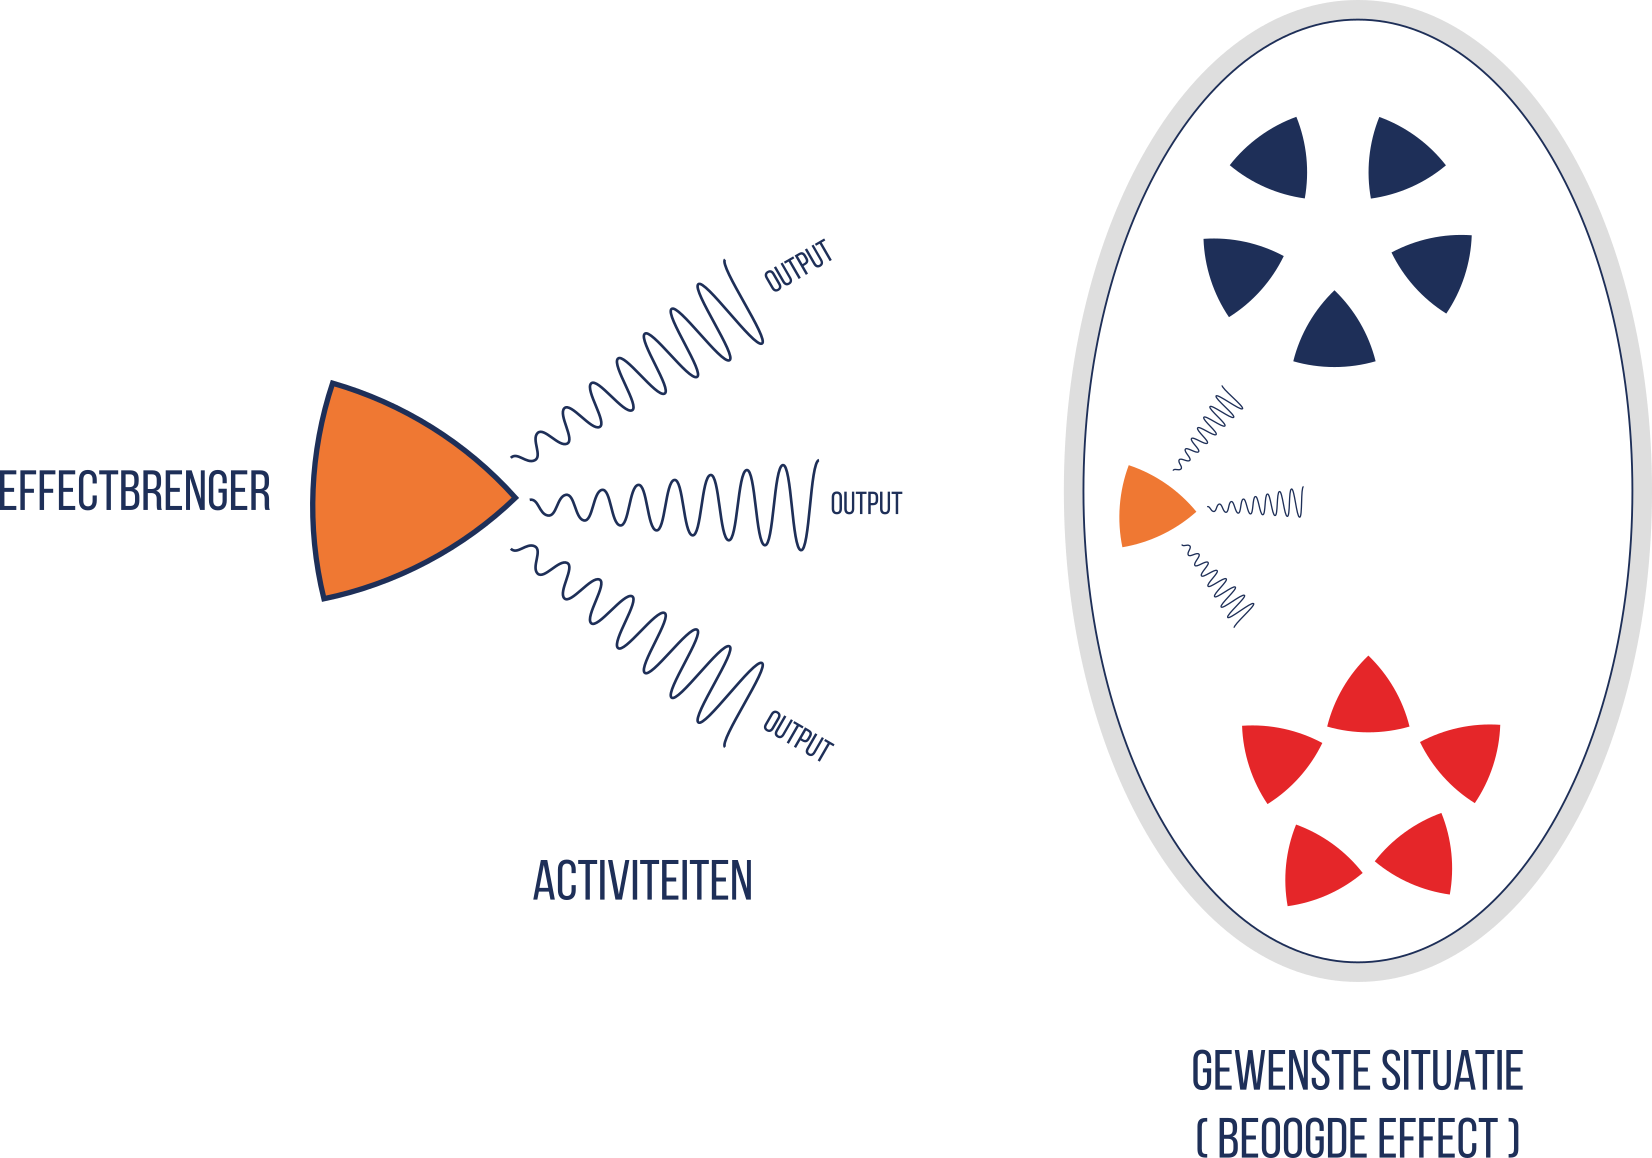
\includegraphics[width=450pt]{data/images/20210324-MDI-effectbrenger-ei} \caption{ }\label{fig:unnamed-chunk-19}
\end{figure}

Bij het ontwikkelen en experimenteren van nieuwe effectbrengers betrekken we het innovatieve vermogen wat buiten de Defensie organisatie ligt. Om de juiste partners te vinden is het belangrijk een duidelijke vraag te stellen. Dat begint met het spreken van eenzelfde taal en het begrijpen van je eigen behoefte. De ervaringen die we daarin maakte zijn verwerkt in het canvas `vraag articulatie.' Aan de hand van het canvas weet de trajectbegeleider, kenniswerker en ervaringsdeskundige een compleet beeld te schetsen van de probleemcontext, probleem en de uitdaging voor de organisatie. Vanuit dat beeld formuleren we samen met interne specialisten de markt-, onderzoek- of ontwerpvragen.

De centrale deelvragen in deze activiteit zijn:

\begin{enumerate}
\def\labelenumi{\arabic{enumi}.}
\tightlist
\item
  Wat is de operationele context?
\item
  Wat is het probleem of kans of risico (in de context)?
\item
  Wat is de uitdaging (voor de organisatie)?
\item
  Wat is je oplossingsrichting?
\item
  Wat is je vraag?
\end{enumerate}

In een forecasting leiden deze vragen tot een schets van de huidige context met een specifiek probleem en een beoogde effectbrenger. Ook wordt duidelijk waarom dit idee niet door de eigen organisatie of eenheid is op te lossen.

In een backcasting resulteren deze vragen in een geschetste toekomstige context (\ref{toekomstige-context}) waarin een effectbrenger zal acteren.

Vraagarticulatie leidt tot een duidelijker beeld van de beoogde effectbrenger en de positie die deze effectbrenger heeft --of kan krijgen-- in de bestaande organisatie.

\href{data/images/20200116-CDE-canvassen-vraagarticulatie.svg}{Canvas vraag articulatie}

\hypertarget{traject-organiseren}{%
\subsection{traject organiseren}\label{traject-organiseren}}

\begin{figure}
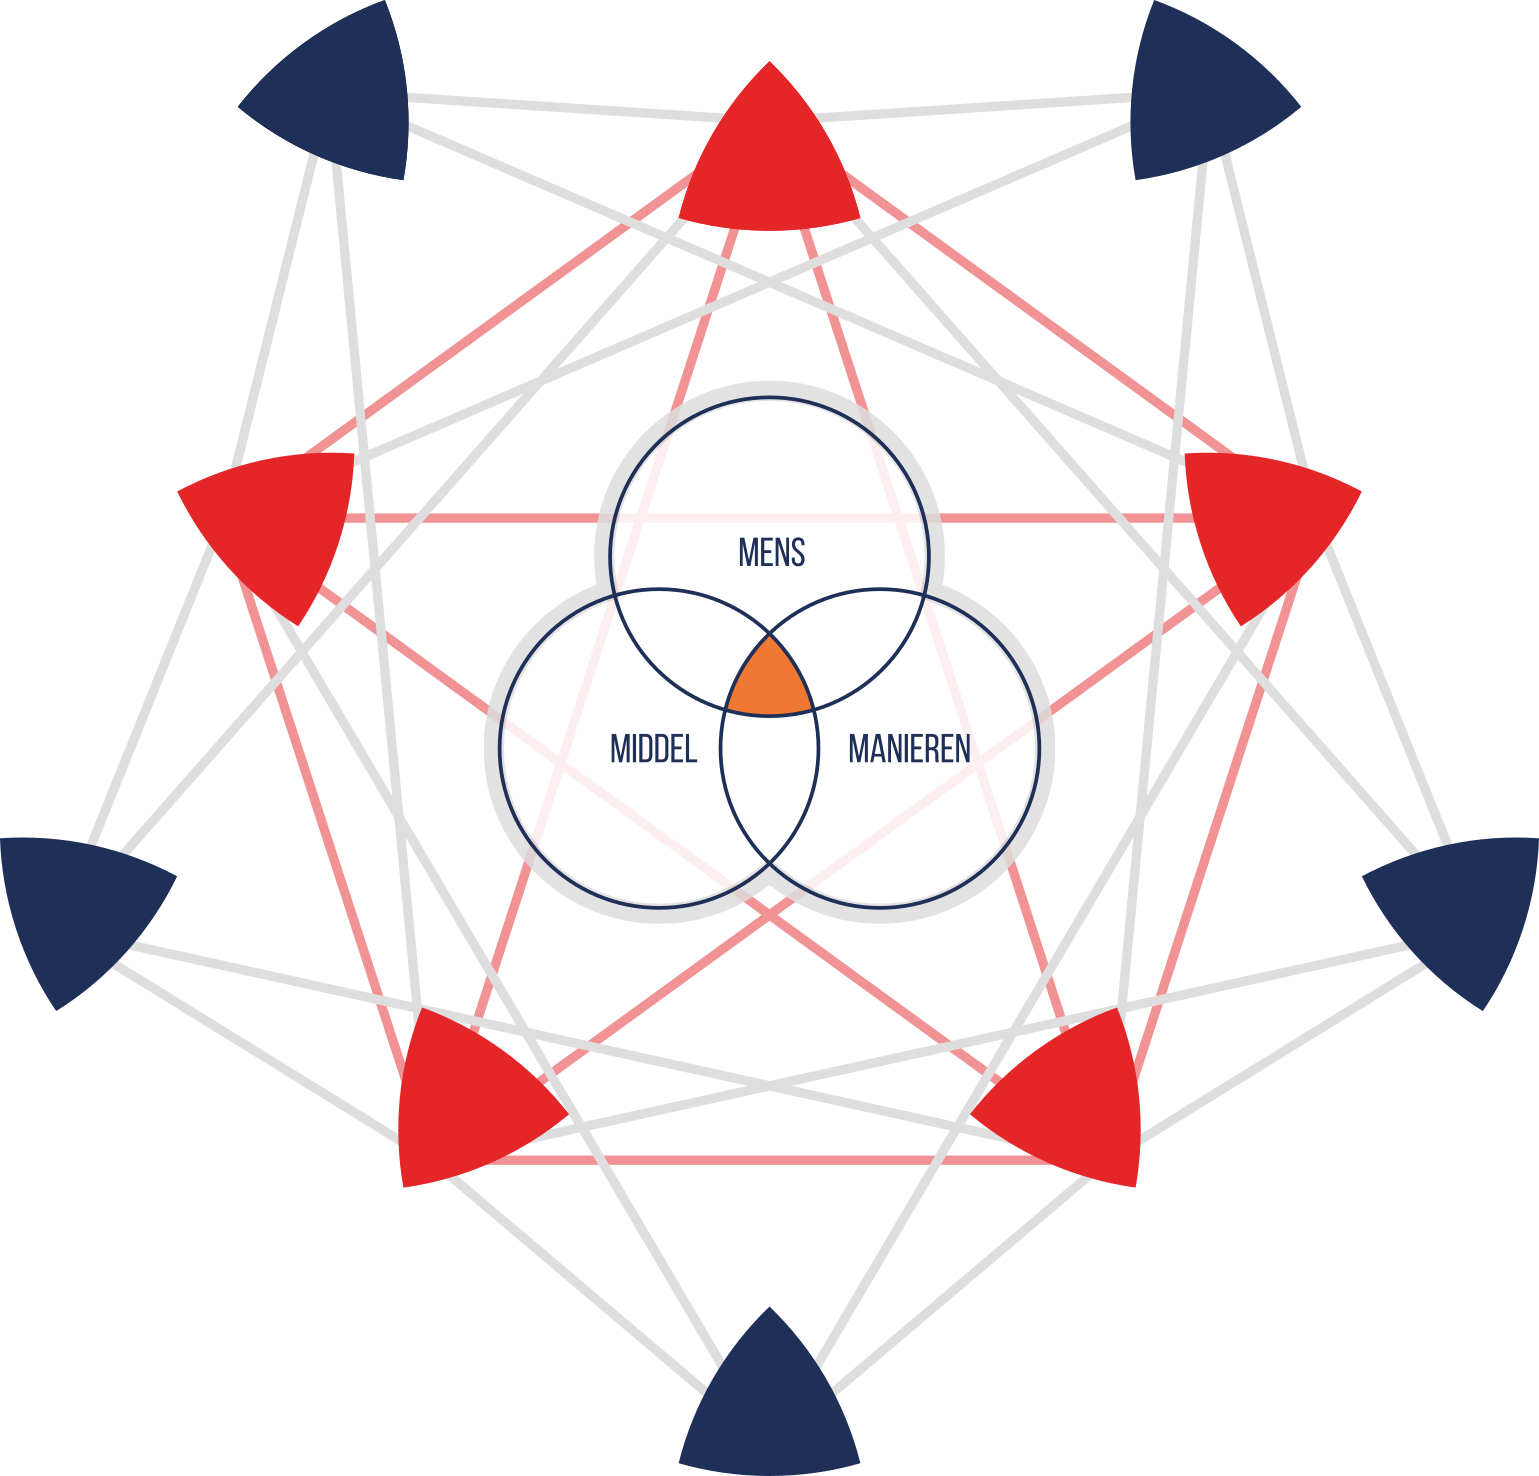
\includegraphics[width=350pt]{data/images/20210401-MDI-trajectorganiseren} \caption{ }\label{fig:unnamed-chunk-20}
\end{figure}

Rondom een ambitie of idee is een netwerk nodig wat dit idee gaat realiseren. Een tijdelijk netwerk met een eigenaar, projectleider, inkoper, producent, dienstverlener en/of kenniswerker, maar ook een experimenteeromgeving, middelen en/of kennis. Deze actoren en factoren worden samengebracht in een projectorganisatie. Zij organiseren samen alle noodzakelijke activiteiten om het idee te ontwikkelen, experimenteren en valideren.

De ervaringen om een projectorganisatie op te zetten zijn verwerk in het canvas `traject organiseren.' Aan de hand van het canvas weet de trajectbegeleider, kenniswerker en ervaringsdeskundige een `business-' of `valueproposition' te schetsen waarmee relevante actoren worden benaderd.

De centrale deelvragen in deze activiteit zijn:

\begin{enumerate}
\def\labelenumi{\arabic{enumi}.}
\tightlist
\item
  Wat zijn de benodigde key resources?
\item
  Wat zijn de key activities?
\item
  Wie zijn de key partners?
\item
  Wat zijn de voorziene kosten of investeringen?
\item
  Wat is de impact van het project op verschillende levels, contexten of niveau's?
\item
  Hoe zijn de actoren gepositioneerd in de actorenroos?
\item
  Wat zijn de relevante aspecten voor het experiment en de experimenteeromgeving?
\end{enumerate}

Traject organiseren leidt tot een duidelijker beeld van de relevante actoren, zoals kenniseigenaar, projectleider, probleem-eigenaar, werkgever (i.r.t. bedrijfsveiligheid) en experimenteer-omgeving. In deze activiteit wordt ook de `verwerving en levering' voor het project voorbereid. Adviseur worden geconsulteerd om te anticiperen op potentiële hindernissen in het vervolgtraject en de implementatie.

\href{data/images/20200116-CDE-canvassen-trajectorganisatie.svg}{Canvas traject organisatie}

\hypertarget{verwerving-en-levering}{%
\subsection{verwerving en levering}\label{verwerving-en-levering}}

Om kort-cyclisch te moderniseren moeten randvoorwaarden worden ingericht die niet beschikbaar zijn in de bestaande organisatie. Dit leidt tot een behoefte aan producten, diensten of partnerschappen. Deze worden voor de duur van het traject verworven door onze dedicated inkopers.

Een inkoopadviseur of inkoper adviseert (en bepaald) de verwervingsstrategie. De betrokkenheid van de inkoper vanaf de start van het traject zorgt voor de snelst mogelijke aanvang van de wettelijke procestijd. Met deze korte lijn krijgen we snelheid en houden we controle in de verwerving en levering. Ook zorgen korte lijnen en nauwe samenwerking met inkoop voor vertrouwen en mogelijkheden om andere dan de meest geeigende inkoopstrategiëen toe te passen.

Voor een betrouwbaar inkoopproces is het noodzakelijk om binnen de wet- en regelgeving te opereren. Tot nu toe bieden de dertien inkoopstrategieën altijd een oplossing voor verwerving. De meest effectieve strategie draagt zorg voor een mogelijke implementatie van het design-concept in de toekomst.

In tegenstelling tot de meeste inkooptrajecten wordt binnen Military Design \& Innovation het inkopen, leveren en contractmanagement onder directe regie van hetzelfde projectteam uitgevoerd. Ook dit draagt bij aan de voortgang van het traject.

\hypertarget{regisseren}{%
\section{regisseren}\label{regisseren}}

onder constructie:
traject- en procesregie en projectbegeleiding.

\hypertarget{continue-dialoog}{%
\subsection{continue dialoog}\label{continue-dialoog}}

\begin{figure}
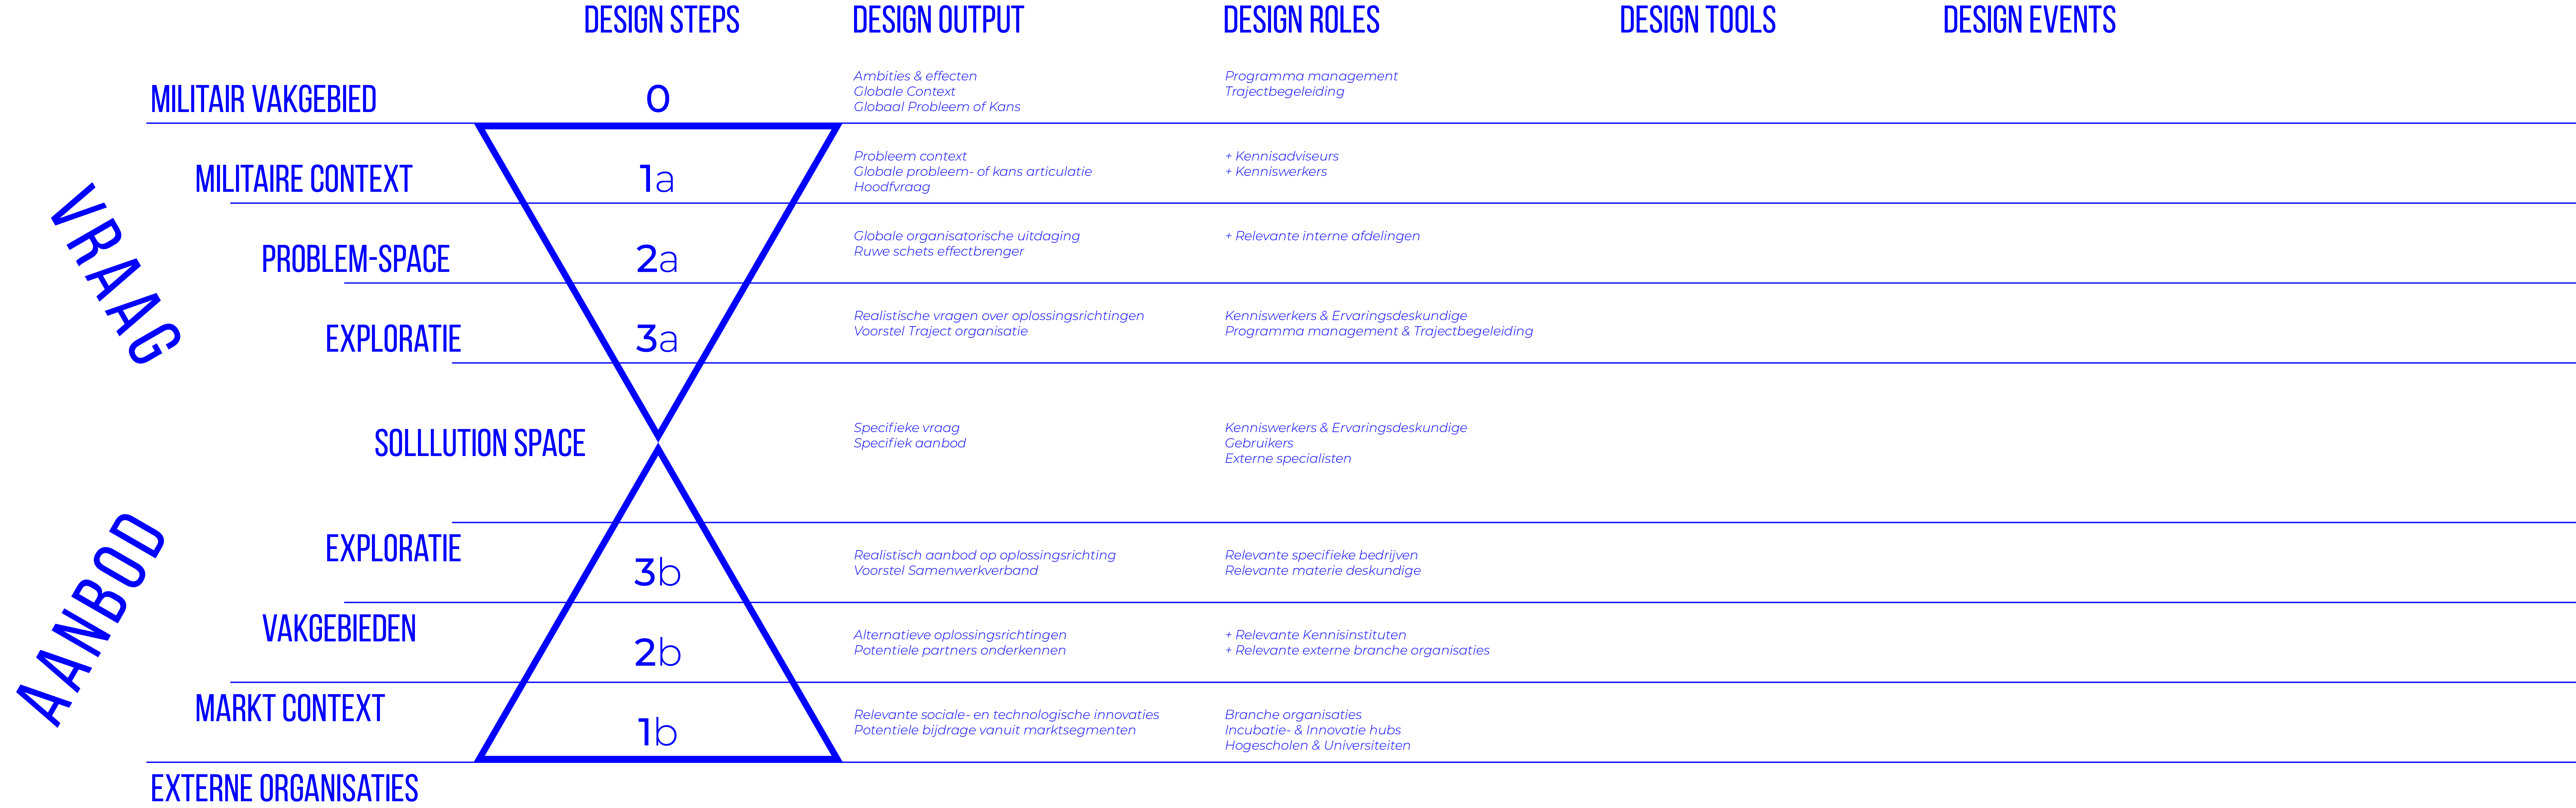
\includegraphics[width=116.58in]{data/images/20200426-CDE-designproces_vraag-aanbod-exploratie_blauwdruk-v2} \caption{Eerste schets van het concept vraag-aanbod exploratie zoals toegepast in de dialoog }\label{fig:vraag-aanbod}
\end{figure}

Met de `continue dialoog' worden externe partijen in een vroegtijdig stadium betrokken in een thematisch programma of bij een technisch vraagstuk. De `continue dialoog' kent een aantal stadia waarin het vraagstuk steeds concreter wordt met hulp van de externe partijen. Figuur \ref{fig:vraag-aanbod} visualiseert een dialoog naar vraagarticulatie en aanbodspecificatie. Het toelopen van de lijnen naar het middelpunt suggereert het convergerend werken in een aantal werksessies of stappen naar het punt waarop de vraagarticulatie en aanbodspecificatie elkaar vinden.

Afhankelijk van het vraagstuk en de context worden relevante partijen door SBID-medewerkers gekoppeld aan de dialoog. De verantwoordelijk programma-manager voert de regie in de dialoog en draagt deze in een latere fase over aan de trajectbegeleider.

\hypertarget{cde-routines}{%
\chapter{CD\&E routines}\label{cde-routines}}

\begin{figure}
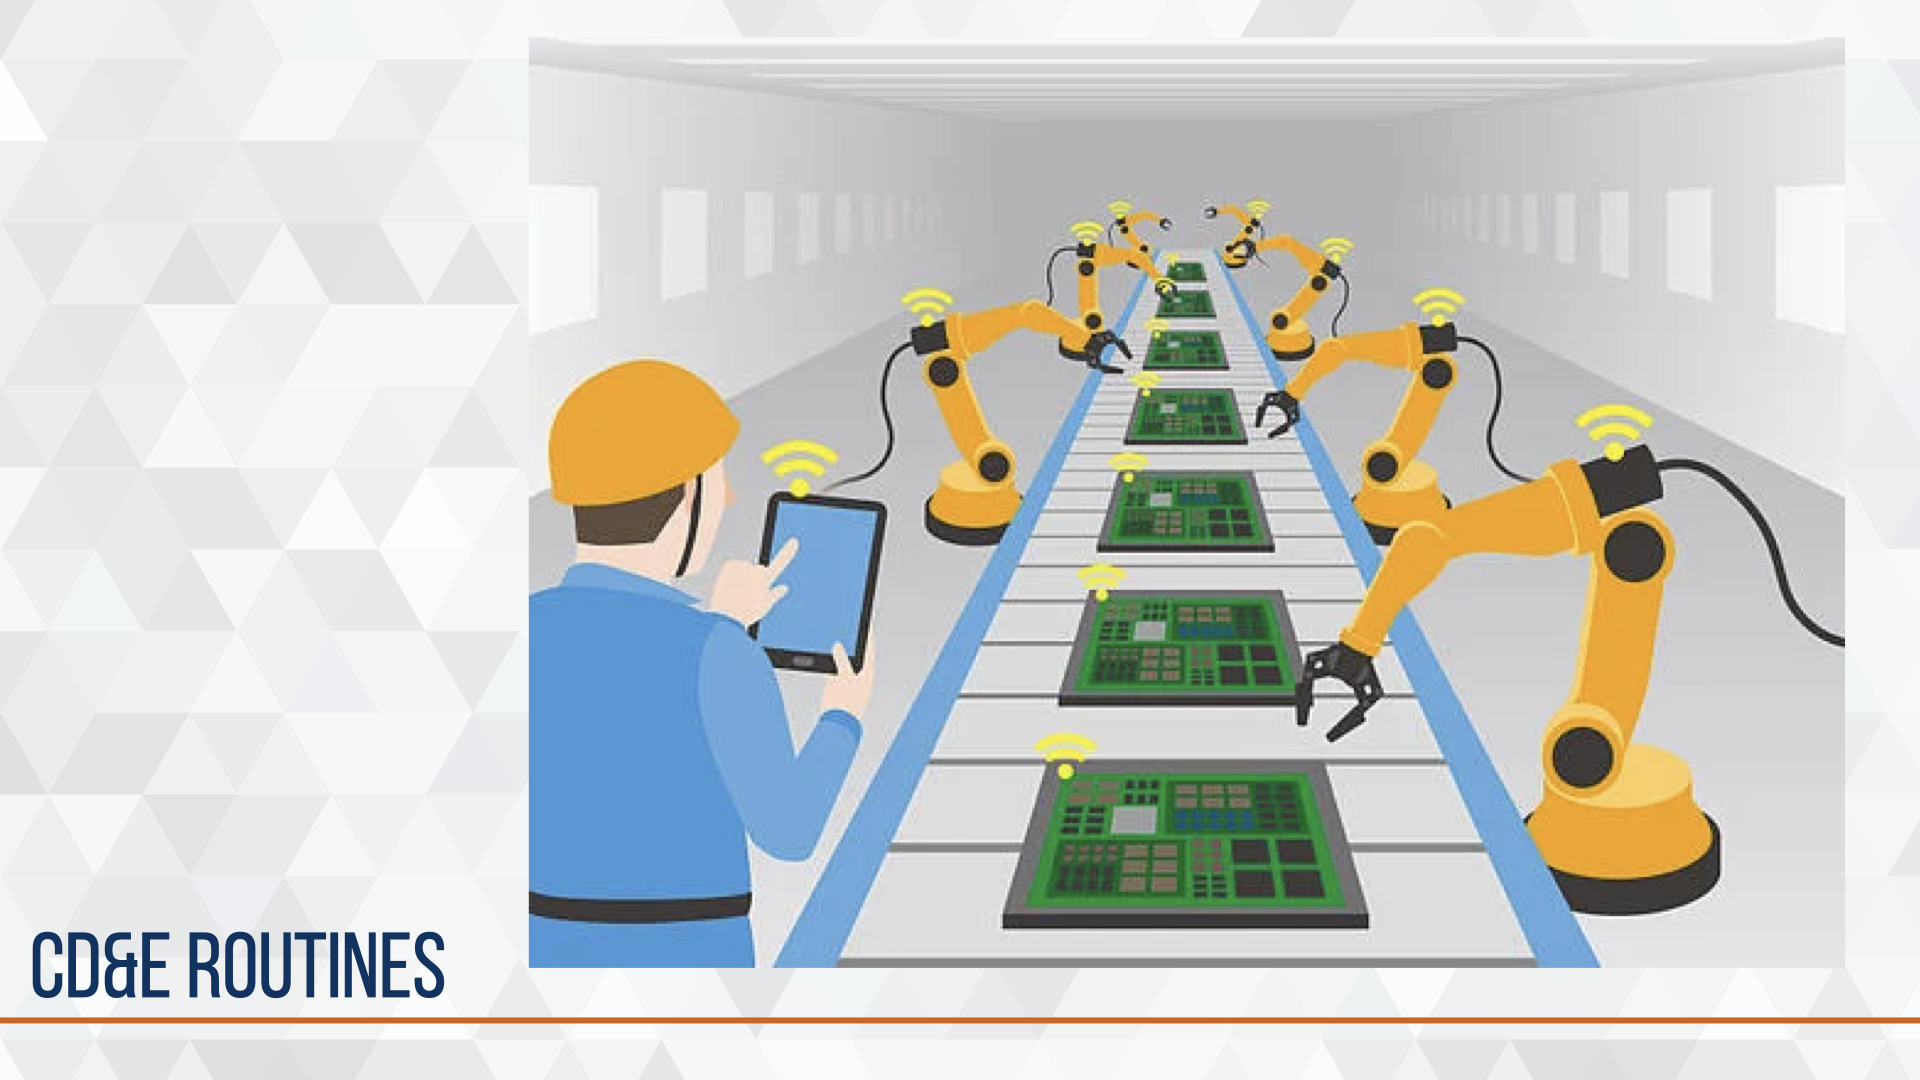
\includegraphics[width=26.67in]{data/keynote-slides/20200430-CDE-Designprocess/20200430-CDE-Designprocess.034} \caption{ }\label{fig:unnamed-chunk-22}
\end{figure}

In 2019 was het CD\&E- budget gestegen tot €20M en was het portfolio voor het eerst groter dan het budget, €24M in 200+ projecten. We hebben ons gedwongen tot het ---laten--- maken van keuzen over de noodzaak, urgentie en haalbaarheid van de lopende projecten en nieuwe voorstellen. Dit proces betekende een herijking van de CD\&E-inspanningen en vroeg om het beschouwen op de toetsingscriteria en fundamentele vragen over responsibility, accountability, projectduur en waarden van een project voor de organisatie.

Daarbij moet in ogenschouw genomen worden dat we een bureaucratische overheidsorganisatie zijn en derhalve te maken hebben met kenmerken als `ministeriële verantwoordelijkheid,' 'continue verantwoording van uitgaven' en `aanbestedende dienst.' Ook de signaalwerking naar de eigenaren van de projecten is van belang. Initiatieven mogen niet worden ontmoedigt maar alles goedkeuren behoorde tot het verleden.

Een herijkingsproces diende daardoor reproduceerbaar en uitlegbaar te zijn aan alle betrokken partijen tot aan de Minister. Het proces droeg ook bij aan een besluitvormingsproces voor de fase na herijking, zo ontstond uit de herijking een aantal routines om ook nieuwe voorstellen langs eenzelfde meetlat te leggen.

\hypertarget{communicatie-in-het-cde-traject}{%
\section{communicatie in het CD\&E-traject}\label{communicatie-in-het-cde-traject}}

\begin{figure}
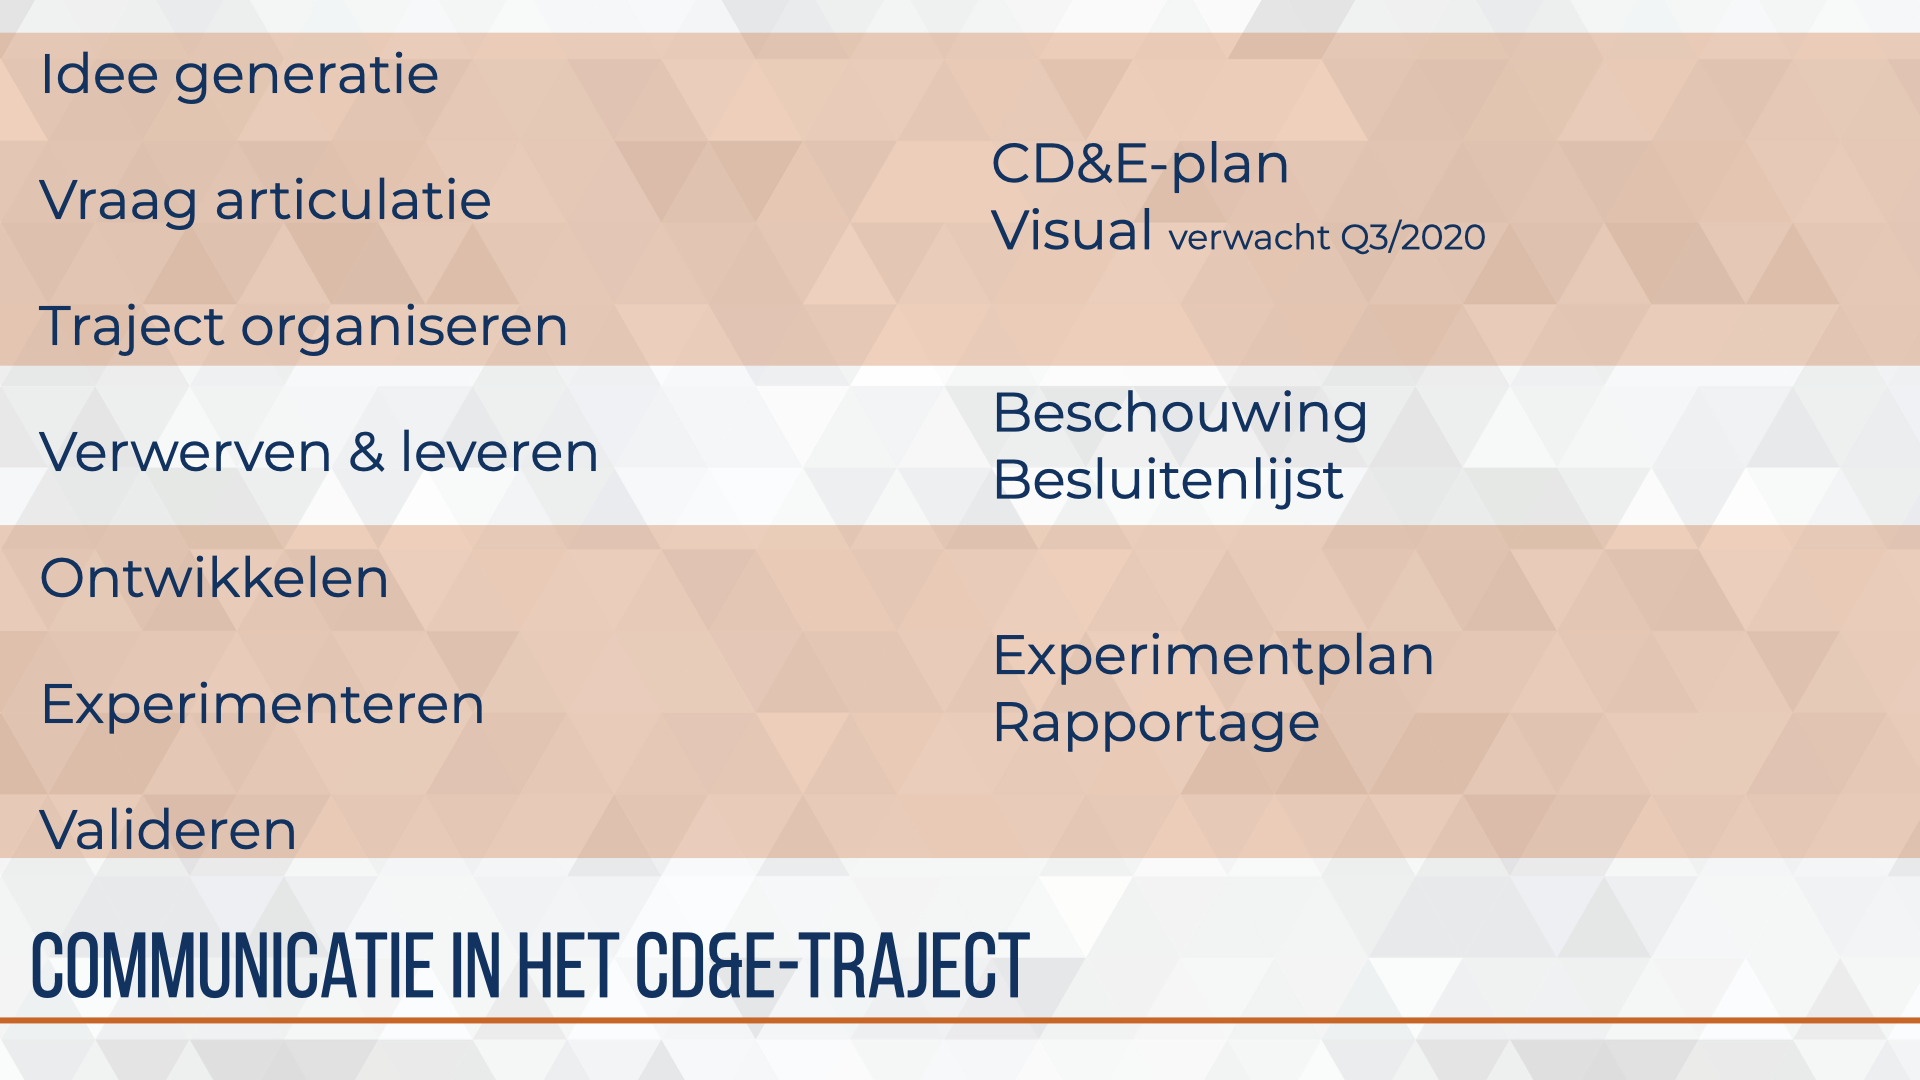
\includegraphics[width=26.67in]{data/keynote-slides/20200430-CDE-Designprocess/20200430-CDE-Designprocess.035} \caption{ }\label{fig:unnamed-chunk-23}
\end{figure}

Om alle belanghebbende te kunnen informeren over het vraagstuk, de aanpak en de uitkomsten worden een aantal documenten gebruikt.
Een CD\&E-plan beschrijft of visualiseert voornamelijk het probleem, probleem-context, vraag, betrokken partijen, projectorganisatie, beoogde effect en globale aanpak voor ontwikkelen, experimenteren en valideren.
Een experimentplan kan later worden opgesteld en beschrijft of visualiseert in detail het experiment en validatie methode. Dit is voornamelijk bedoeld ten behoeve van de project-uitvoering.
Een rapportage communiceert de uitkomsten van een project en moet kunnen dienen als input voor de implementatie.

Na goedkeuring wordt een eventueel verwervingsproces uitgevoerd.

Tijdens het gehele proces wordt de voortgang bewaakt door de trajectbegeleider zodat er één persoon is die van begin tot eind zicht heeft op de ontwikkelingen.

\hypertarget{besluitvorming-trajectvoorstellen}{%
\section{besluitvorming trajectvoorstellen}\label{besluitvorming-trajectvoorstellen}}

\begin{figure}
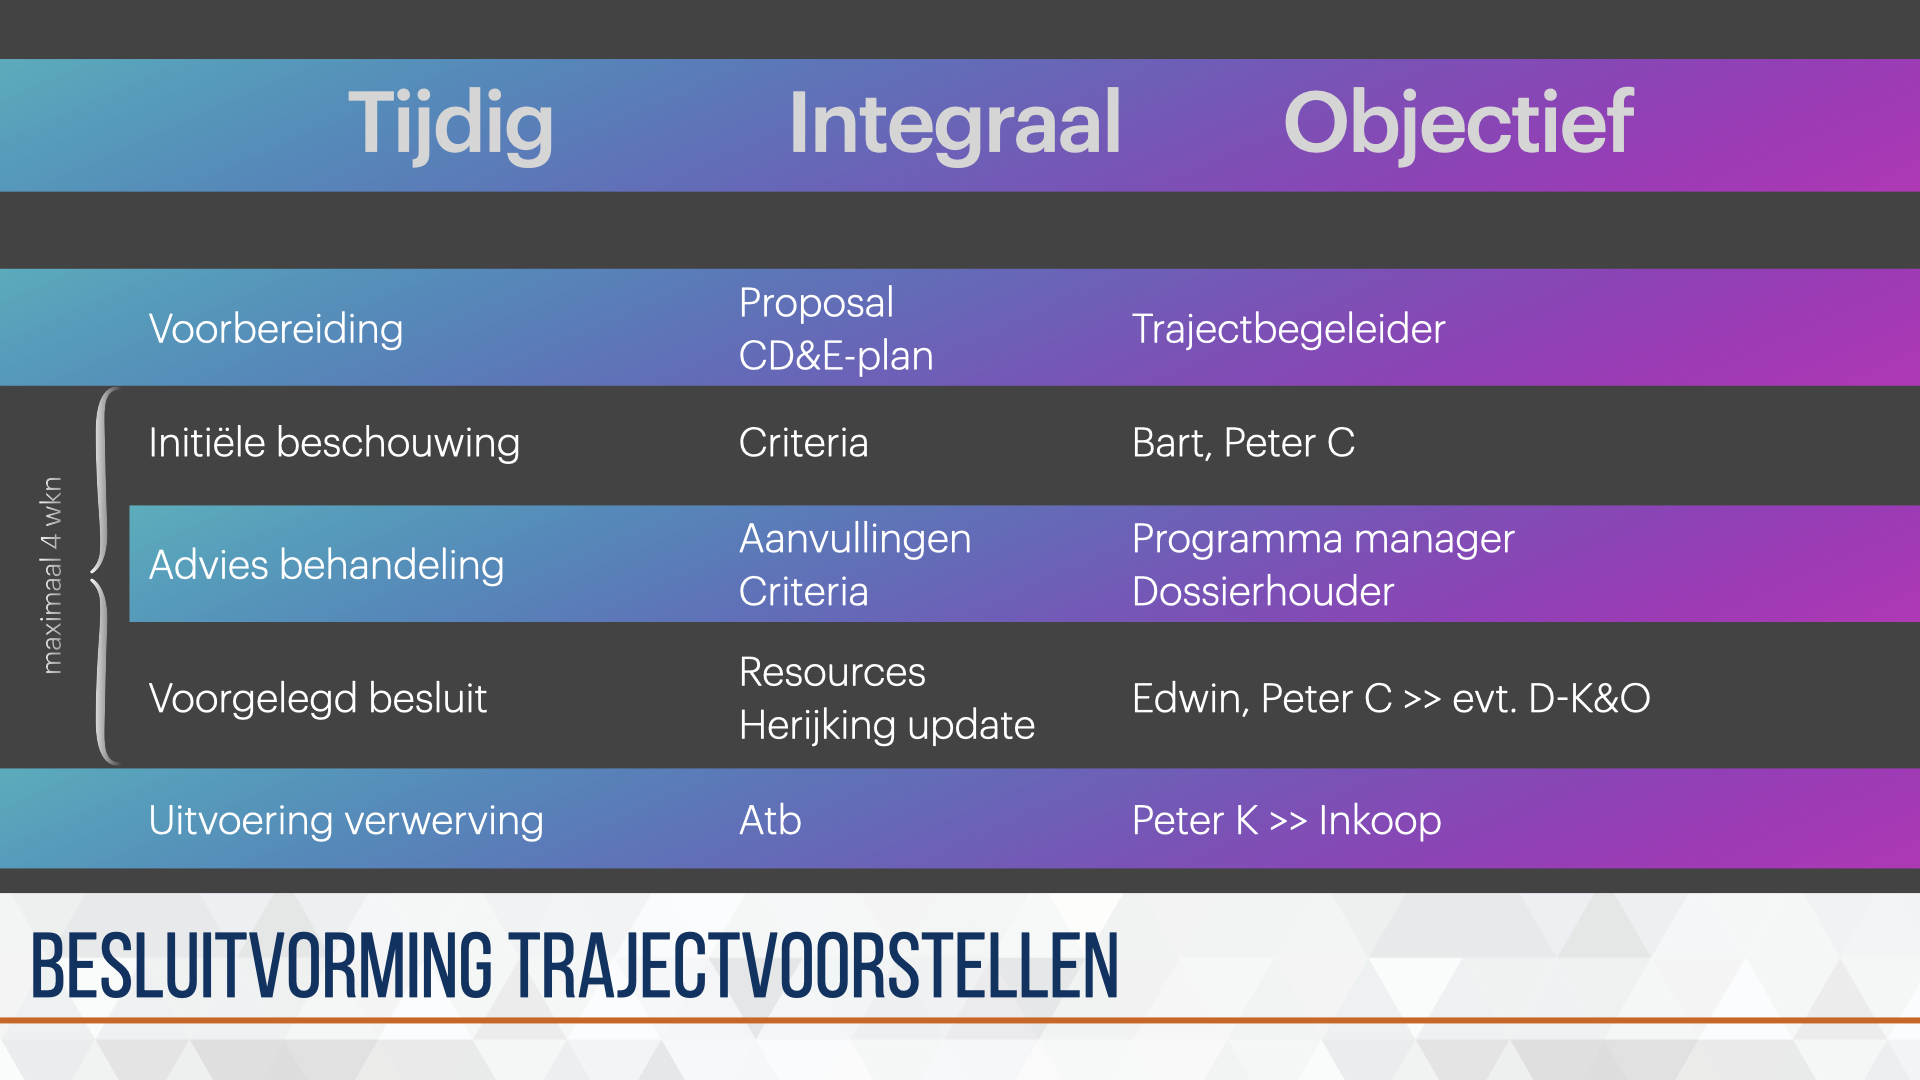
\includegraphics[width=26.67in]{data/keynote-slides/20200430-CDE-Designprocess/20200430-CDE-Designprocess.037} \caption{ }\label{fig:unnamed-chunk-24}
\end{figure}

Voorafgaand aan de besluitvorming wordt een stafadvies opgesteld door de CD\&E trajectbegeleider, S\&P dossierhouder en CD\&E programma-manager. Dit advies ontstaat door het beschouwen van het project-voorstel op de toetsingscriteria en wordt voorbereid en samengevat door de teamleider trajectbegeleiding. De focus ligt op noodzaak en urgentie van het voorstel ten opzichte van staande beleid en visie, veel gebruikte referenties zijn de visie C-LAS ``Veiligheid en vooruitzien'' en het Operationeel kader landoptreden (OKL). Na de inhoudelijke beschouwing worden eventuele financiële middelen toebedeeld.

Besluitvorming over een traject ligt in principe bij de Directeur Kennis \& Ontwikkeling, dankzij de getoonde systematische aanpak is het vertrouwen gegeven om dit binnen CD\&E te beleggen.

\hypertarget{toetsingscriteria}{%
\section{toetsingscriteria}\label{toetsingscriteria}}

\begin{figure}
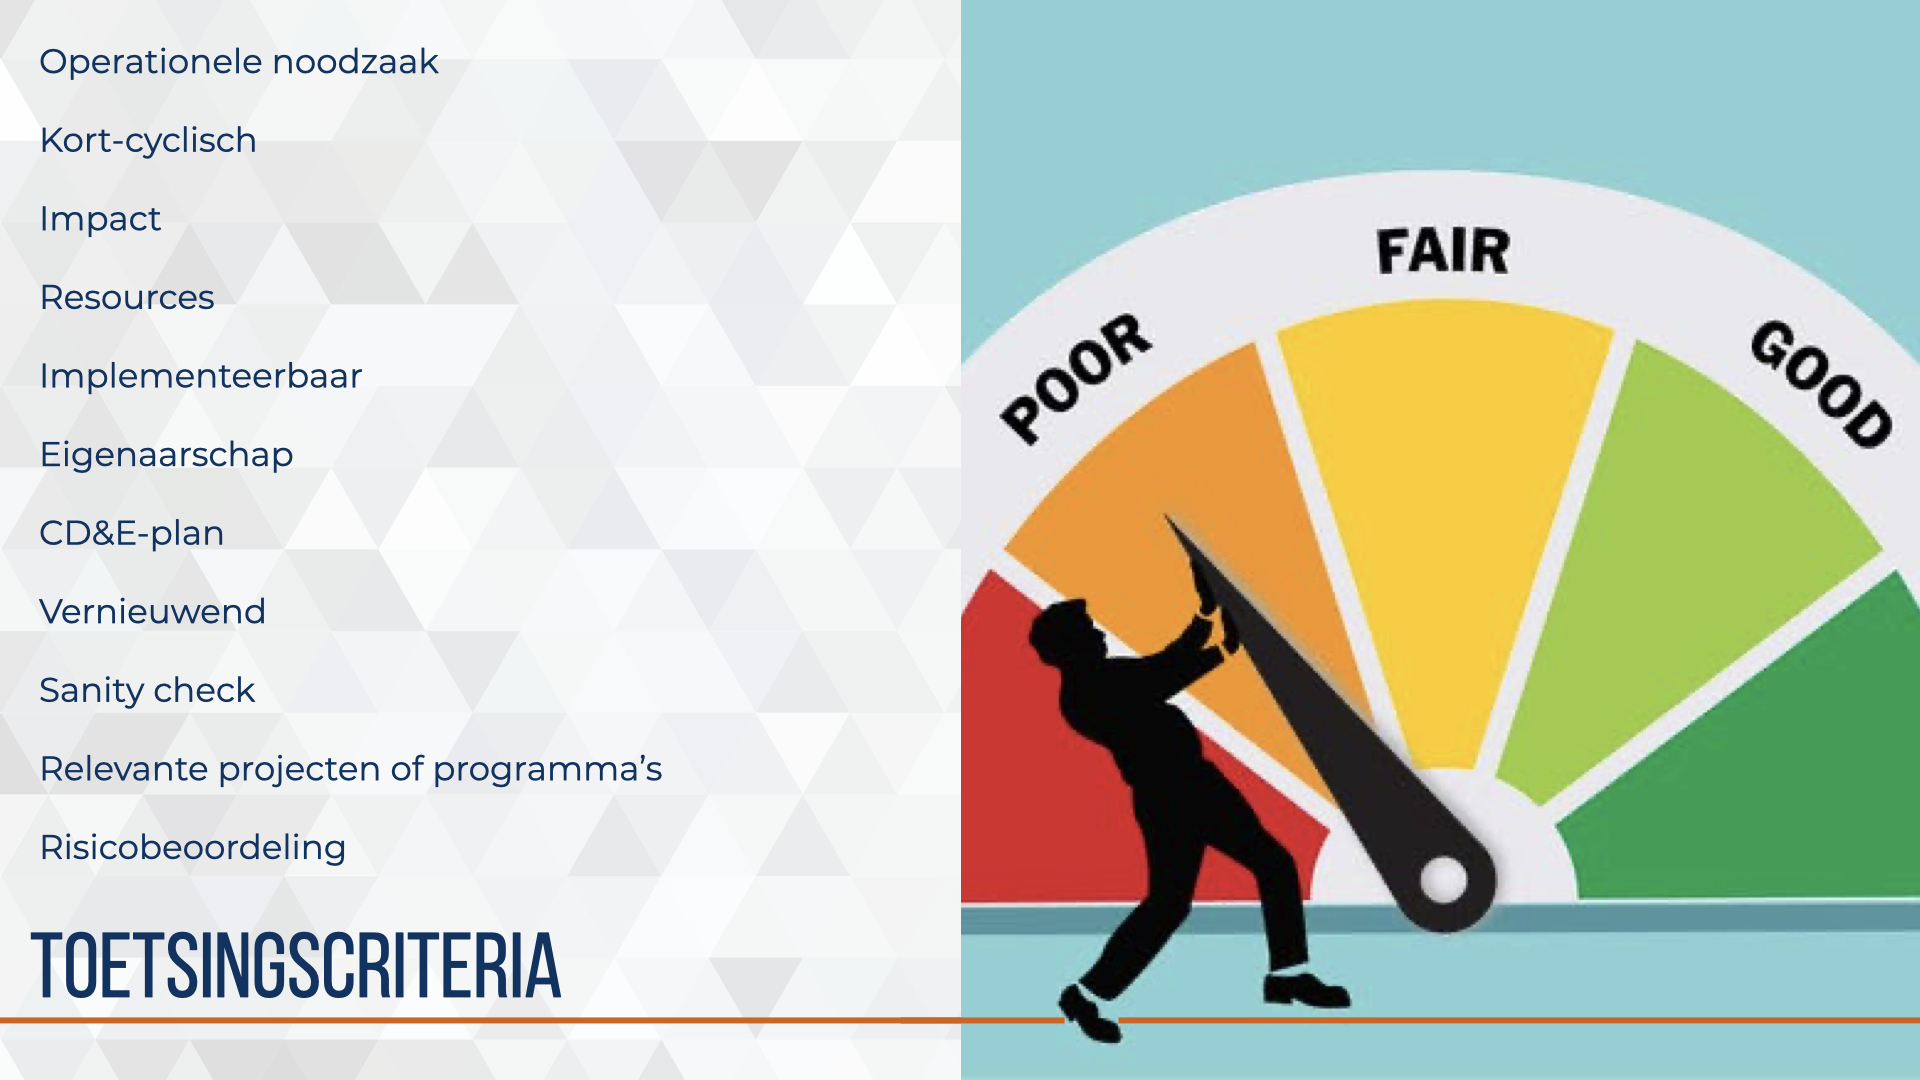
\includegraphics[width=26.67in]{data/keynote-slides/20200430-CDE-Designprocess/20200430-CDE-Designprocess.038} \caption{ }\label{fig:unnamed-chunk-25}
\end{figure}

\hypertarget{cde-process}{%
\chapter{Ontstaansgeschiedenis en doorontwikkeling}\label{cde-process}}

\begin{figure}
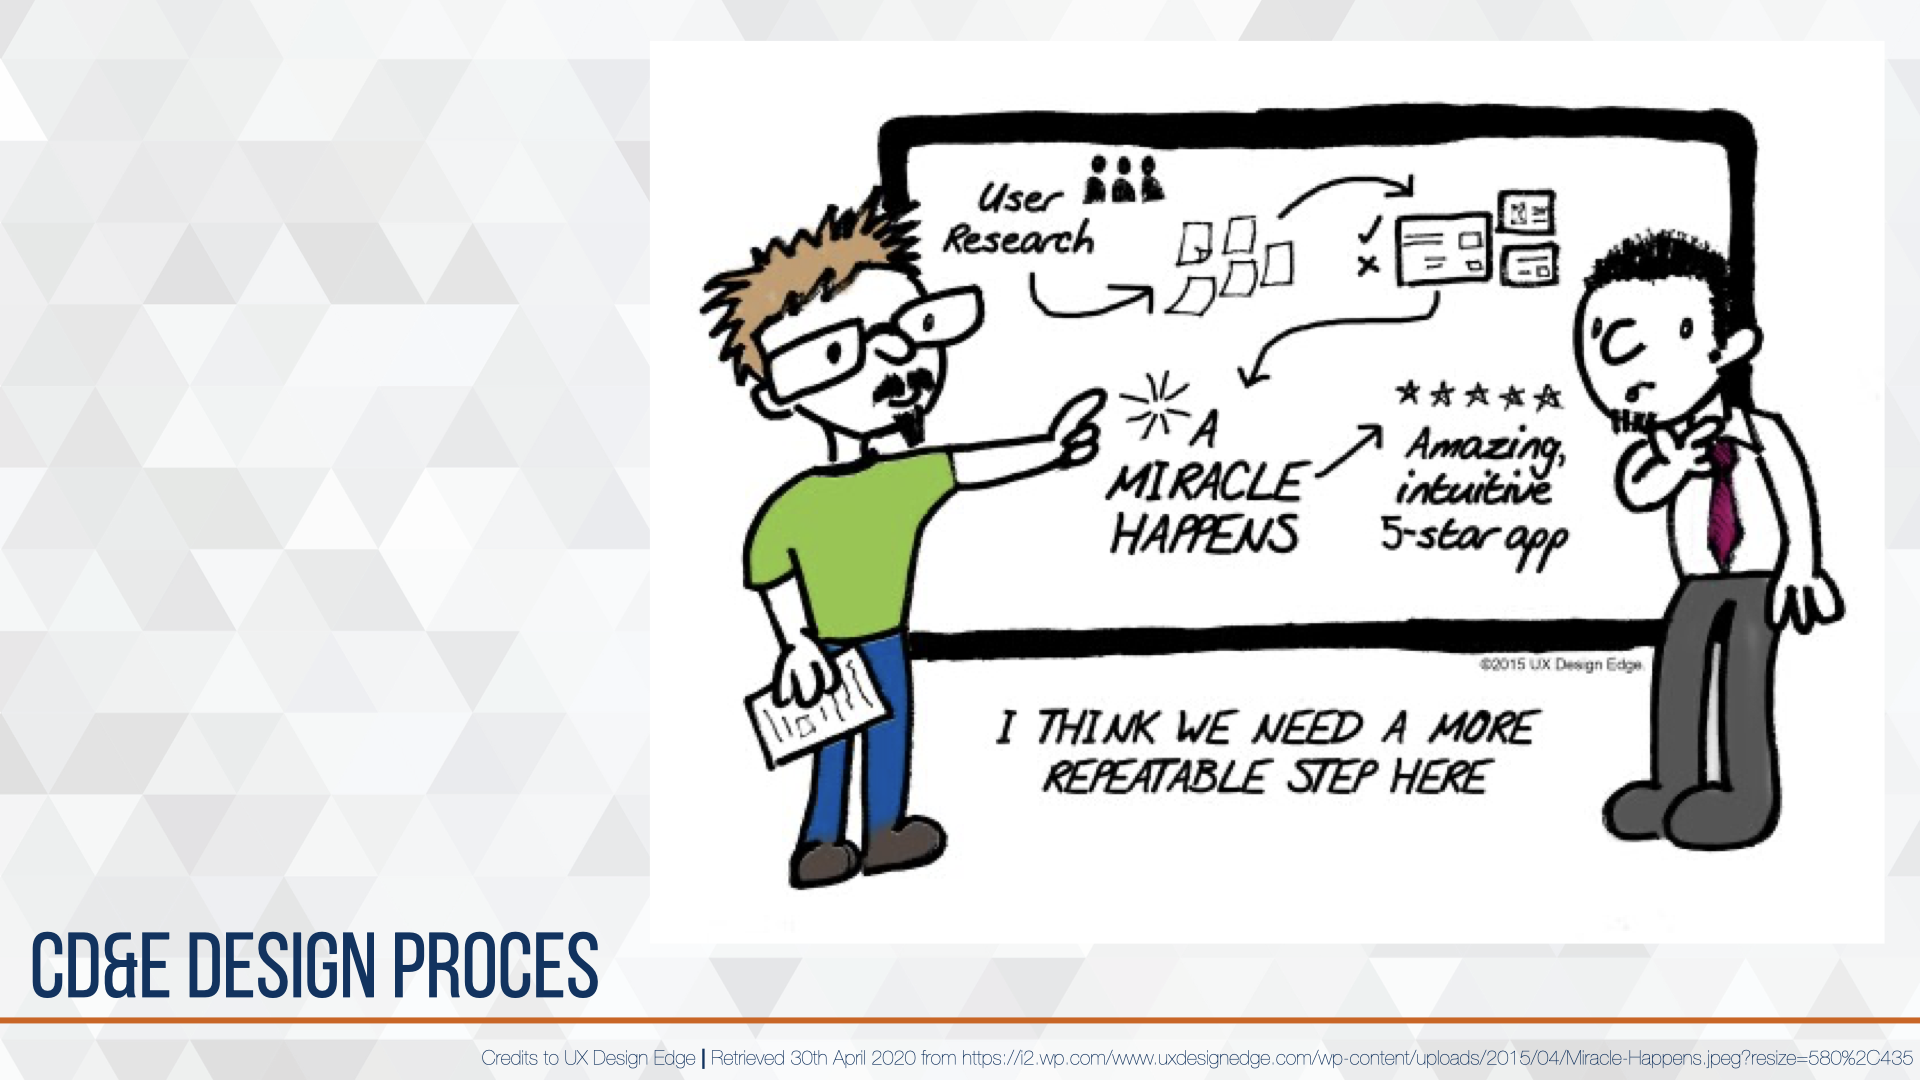
\includegraphics[width=26.67in]{data/keynote-slides/20200430-CDE-Designprocess/20200430-CDE-Designprocess.018} \caption{ }\label{fig:unnamed-chunk-26}
\end{figure}

De organisatorische uitdaging die de kenniswerker en de trajectbegeleiding hebben ligt vooral in de Hoe-vragen. Op welke manier kan de beoogde effectbrenger worden ontworpen, ontwikkeld, getest en geïmplementeerd in de bestaande Landmacht organisatie? Er is geen pasklaar antwoord, maar door de vele trajecten is wel een rode draad te ontdekken en zijn een aantal activiteiten, methoden en instrumenten die effectief blijken en vaker terug komen.

Vanuit deze kennis, vaardigheid en ervaring is het CD\&E design proces ontwikkeld, en wordt het nog regelmatig aangepast, verbeterd en uitgebreid.

Hierna volgen de verschillende bouwstenen die gebuikt kunnen worden om het design proces vorm te geven. De bijzondere volgorde waarin de bouwstenen worden gepresenteerd zijn het meest effectief in de bureaucratische overheidsorganisatie Defensie die tevens als Aanbestedende dienst wordt gekenmerkt in de aanbestedingswet.

\hypertarget{position-into-crafstmen}{%
\section{position into crafstmen}\label{position-into-crafstmen}}

\begin{figure}
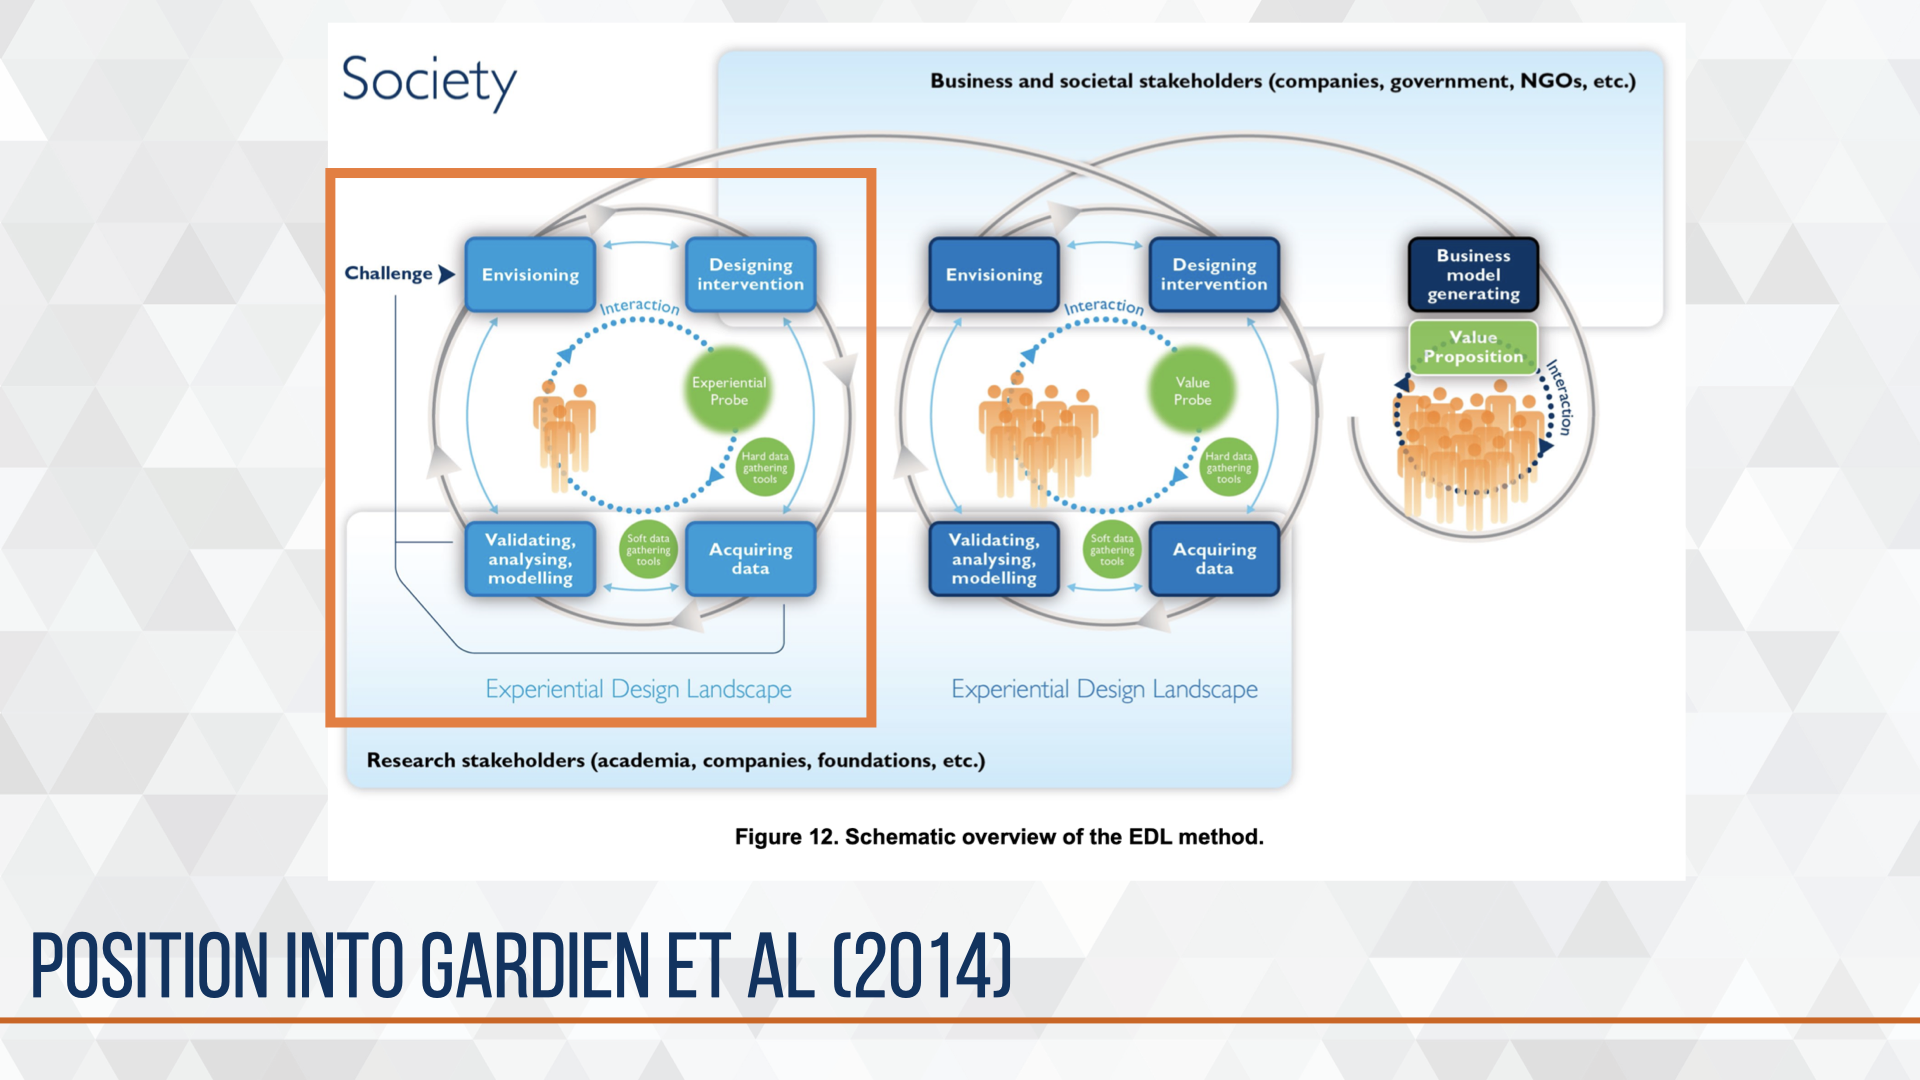
\includegraphics[width=26.67in]{data/keynote-slides/20200430-CDE-Designprocess/20200430-CDE-Designprocess.019} \caption{Het Military Design proces gepositioneerd in het EDL method.}\label{fig:unnamed-chunk-27}
\end{figure}

Positioning the proces into the frame of \protect\hyperlink{ref-gardien_changing_2014}{Gardien et al.} (\protect\hyperlink{ref-gardien_changing_2014}{2014}).

\hypertarget{cde-framework-2017-2018-descriptive}{%
\section{CD\&E framework 2017-2018 (descriptive)}\label{cde-framework-2017-2018-descriptive}}

\begin{figure}
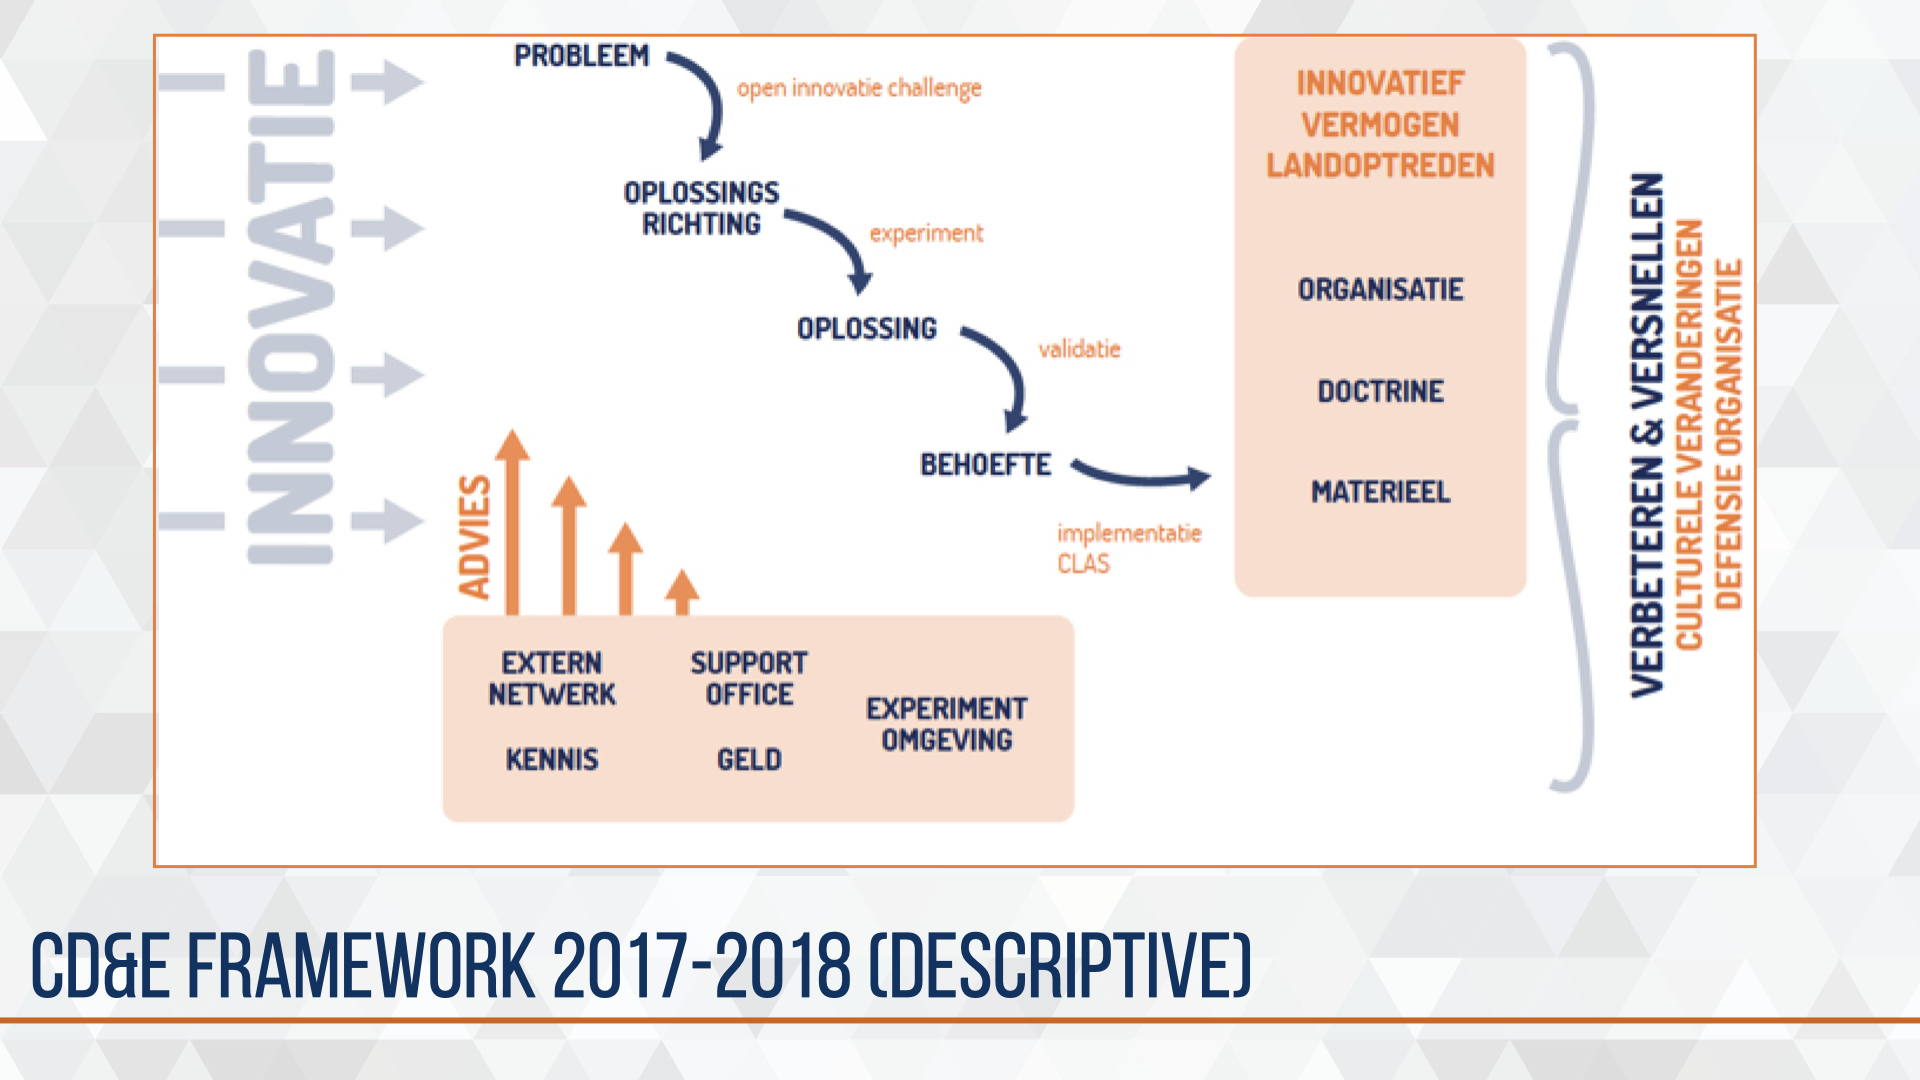
\includegraphics[width=26.67in]{data/keynote-slides/20200430-CDE-Designprocess/20200430-CDE-Designprocess.020} \caption{Eerste schets van het CD\&E design model uit 2018. }\label{fig:unnamed-chunk-28}
\end{figure}

De eerste schets van een framework van de inspanningen voor kort-cyclisch moderniseren voor het landoptreden. In het midden vier fase en stappen om te komen van een probleem naar een implementatie. Onderaan de schets de toenmalige middelen en diensten die door CD\&E beschikbaar werden gesteld. De inspanningen waren gericht op het binnen halen van de externe innovatie (links) en via één of meerdere fase en stappen te brengen naar het vergroten van het innovatief vermogen in het landoptreden op de aspecten organisatie, doctrine en/of materieel. Deze inspanningen dragen uiteindelijk ook bij aan het verbeteren en versnellen van processen en procedures binnen de organisatie met de wens om zelfs culturele verandering te initiëren.

Het eerste framework werd gebruikt in een aantal projecten en bij het intern communiceren ---en eenheid van opvatting creëren--- over de initiatieven voor kort-cyclisch moderniseren in het landoptreden.

Als methodiek is het model van \protect\hyperlink{ref-klinkers_navigeren_2014}{Klinkers et al.} (\protect\hyperlink{ref-klinkers_navigeren_2014}{2014}) toegepast waarin de auteurs spreken van drie licenties. Licence to represent, licence to operate \& licence to innovate.

Vanuit reflection in action ontstond het design-keten-proces, een basis template voor een CD\&E-plan en een gemeenschappelijke taal.

\hypertarget{design-keten-proces-2018-2019}{%
\section{design-keten-proces 2018-2019}\label{design-keten-proces-2018-2019}}

\begin{figure}
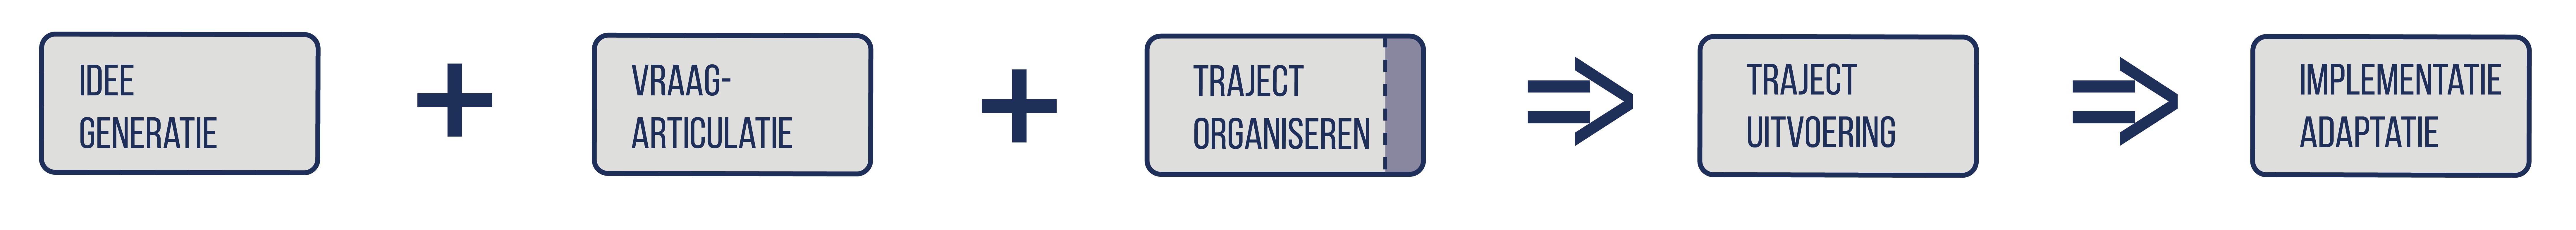
\includegraphics[width=122.31in]{data/images/20190710-CDE-designproces_bouwstenenKeten} \caption{Eerste opzet van MD\&I activiteiten.}\label{fig:unnamed-chunk-29}
\end{figure}

Groei zorgt voor nieuwe uitdagingen, mogelijkheden en mensen. Het aantal moderniseringsvraagstukken steeg en werd gecompliceerder waardoor de noodzaak voor meer trajectbegeleiders ontstond, deze rol werd met prioriteit gevuld. Daarmee ontstond de noodzaak om de opgedane kennis, vaardigheid en ervaring te borgen. Hiervoor is het eerste design-keten-proces en bijhorende canvassen ontworpen, getest en geïmplementeerd in het team.

Voor het ontwerp is gebruik gemaakt van de ervaringen van vier trajectbegeleiders die enige ervaring hadden opgedaan in de periode 2015-2018 met het opstarten en organiseren van moderniseringsvraagstukken.

Bij het testen is gebruik gemaakt van vier nieuwe trajectbegeleiders zonder ervaring op nieuw ingebrachte vraagstukken. Deze vier nieuwe trajectbegeleiders werden opgeleid, getraind, begeleid en gecoacht door één ervaren trajectbegeleider.

Trajecten van idee naar implementatie zijn uniek.
Ieder traject een andere keten van bouwstenen.

\textbf{de eerste canvassen}

\begin{figure}
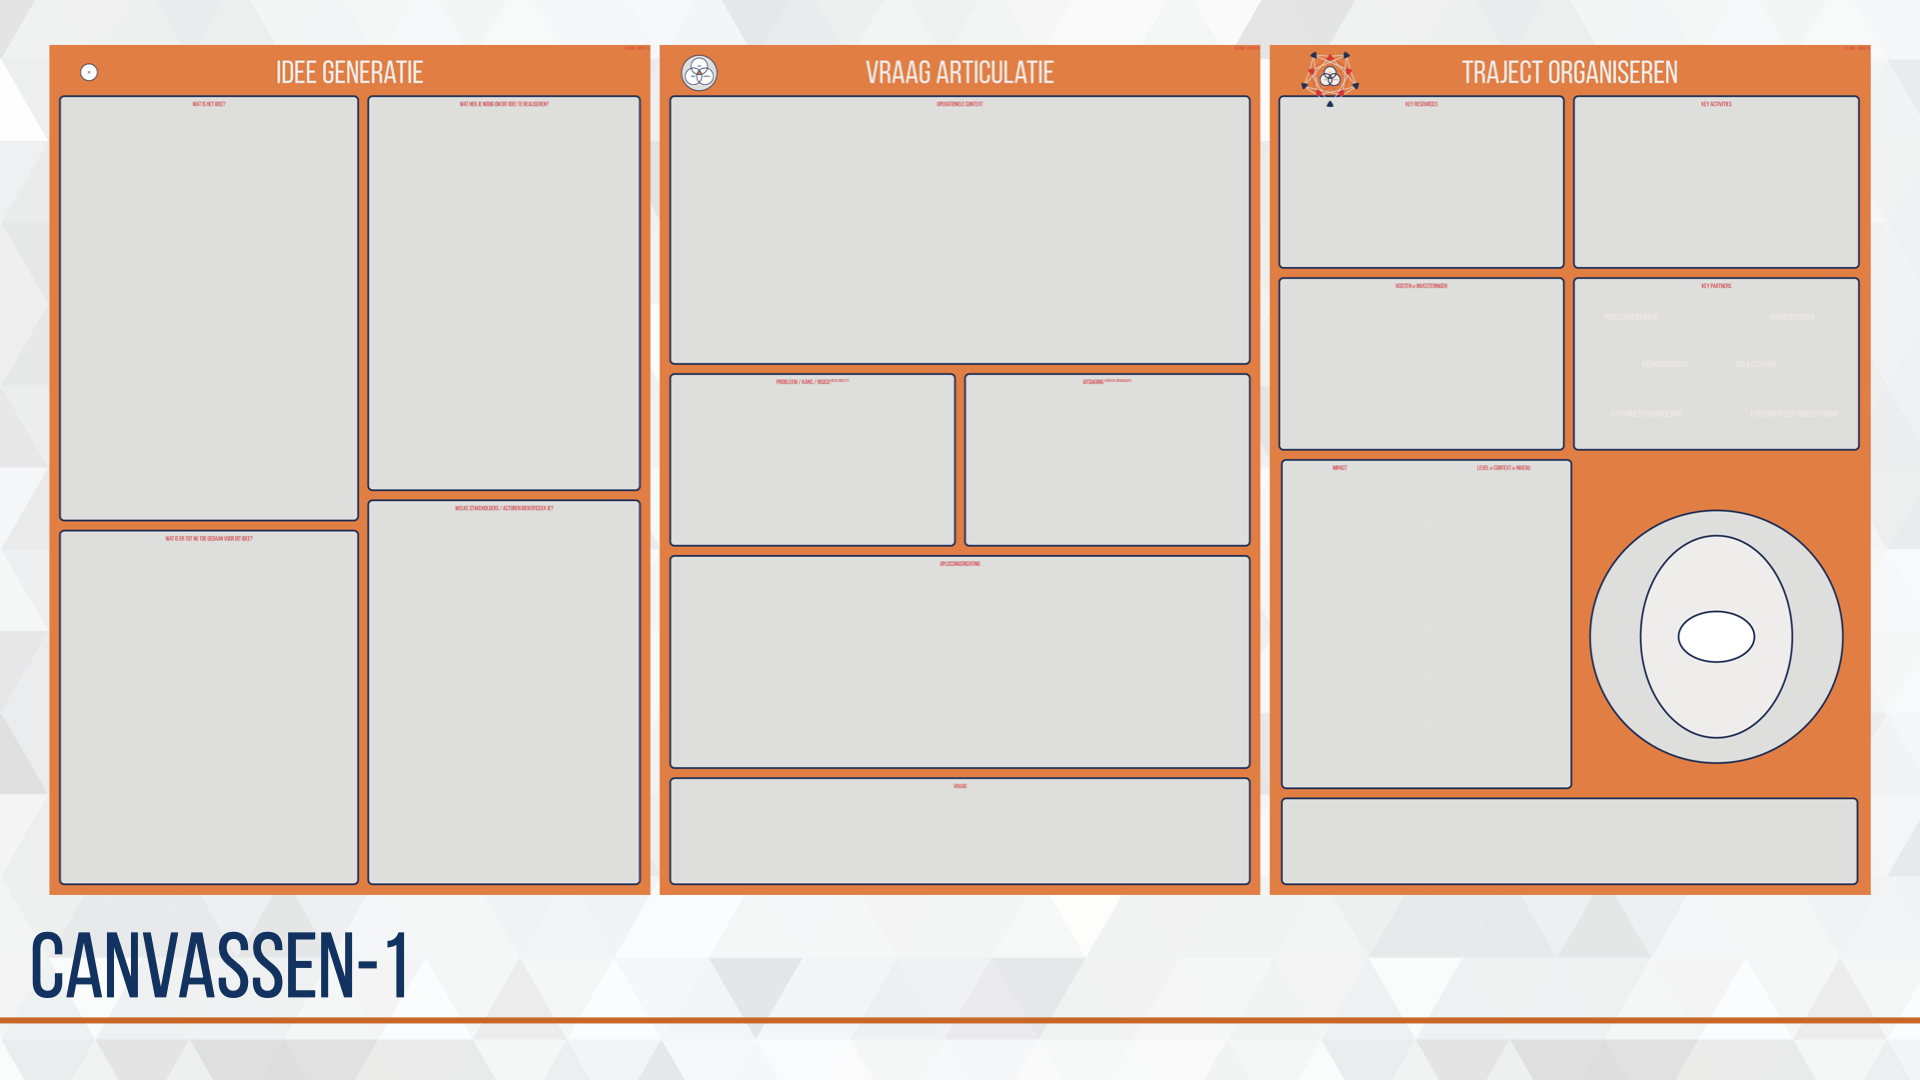
\includegraphics[width=26.67in]{data/keynote-slides/20200430-CDE-Designprocess/20200430-CDE-Designprocess.023} \caption{Eerste canvassen prototype.}\label{fig:unnamed-chunk-30}
\end{figure}

\textbf{toetsingscriteria}

\begin{figure}
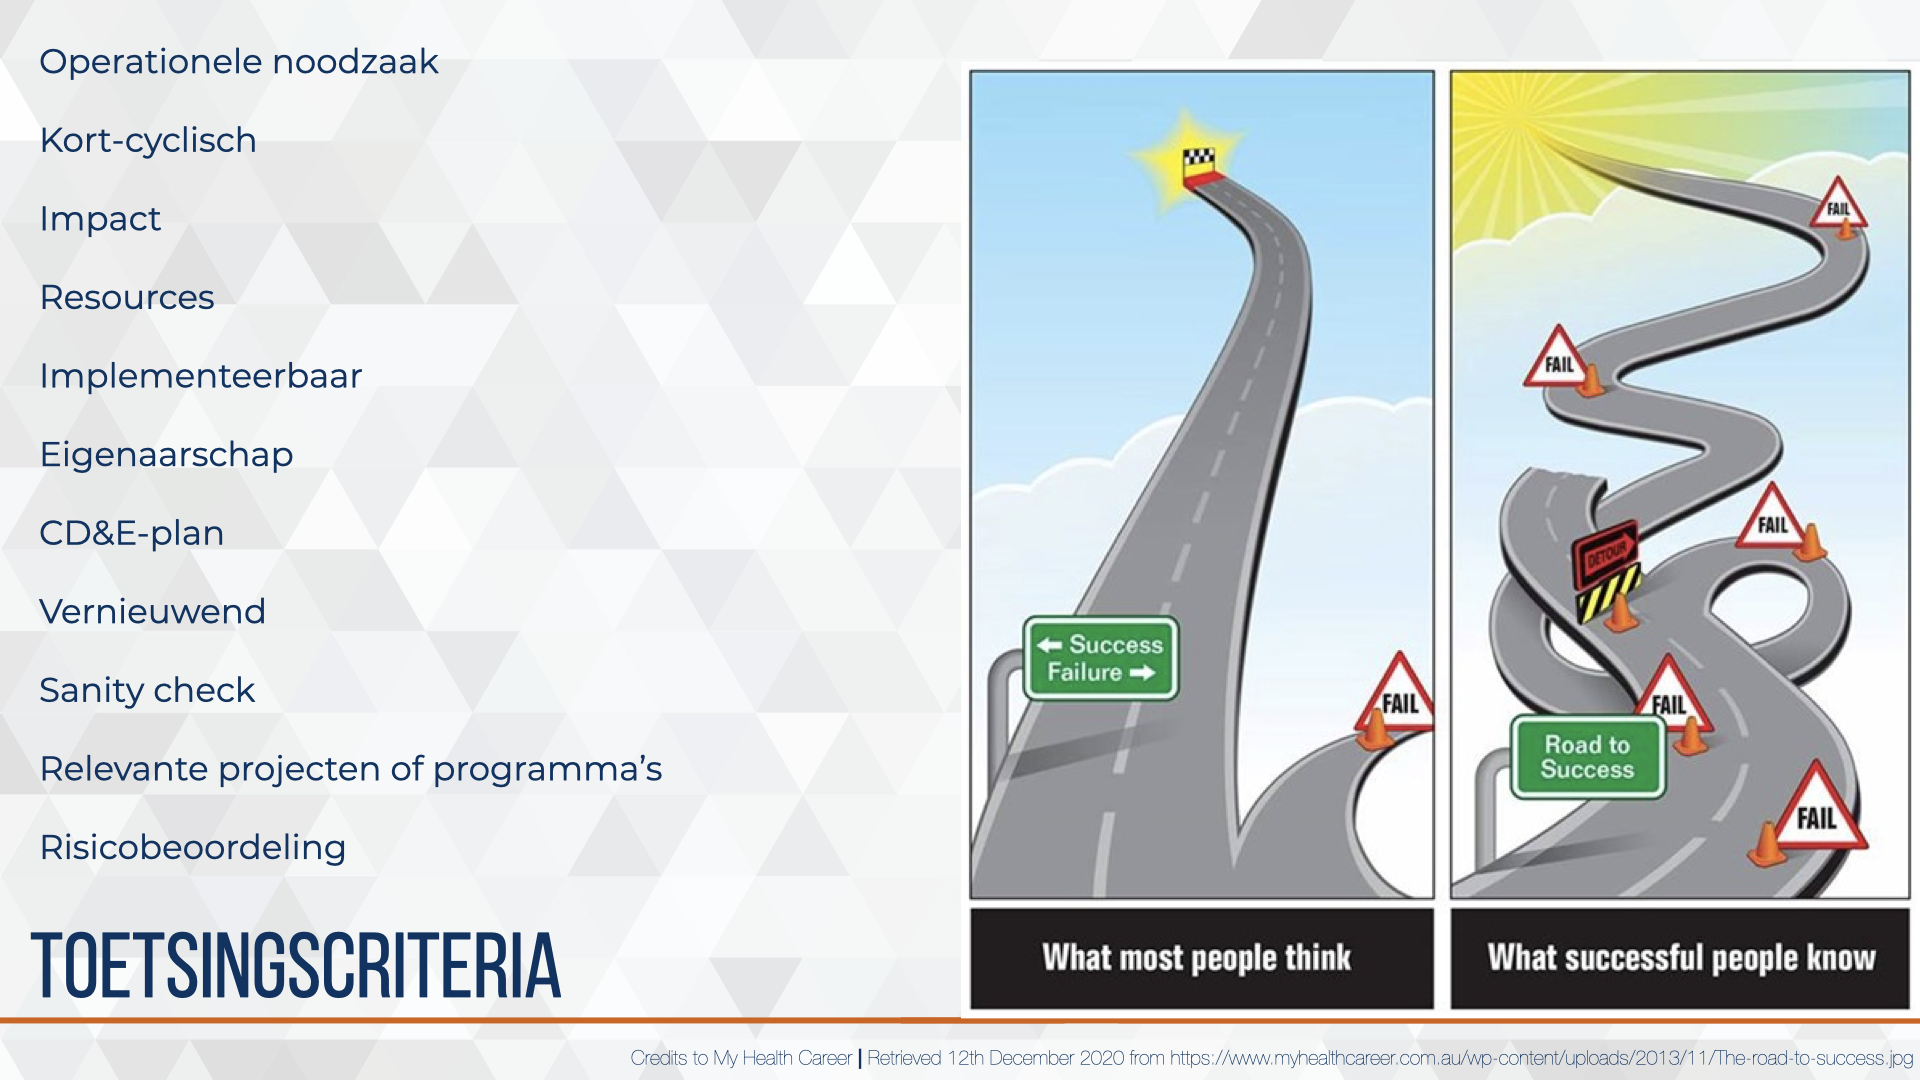
\includegraphics[width=26.67in]{data/keynote-slides/20200430-CDE-Designprocess/20200430-CDE-Designprocess.024} \caption{De indicatoren voor Military Design \& Innovation.}\label{fig:unnamed-chunk-31}
\end{figure}

Naast de canvassen en het mindmodel waren een aantal indicatoren opgesteld. Deze kregen helaas de naam selectie- of toetsingscriteria wat geen recht deed aan de kracht van indicatoren maar verwerd tot een binair goed/fout controle mechanisme. De indicatoren waren door mij opgesteld als reminder of checklist, ze moeten zijn overdacht en besproken in het proces. De mate waarin de indicator is doorgevoerd in het traject kan iets zeggen over de succesfactor op basis van eerdere kennis en ervaring.
\textbf{variaties op denkmodellen}

\begin{figure}
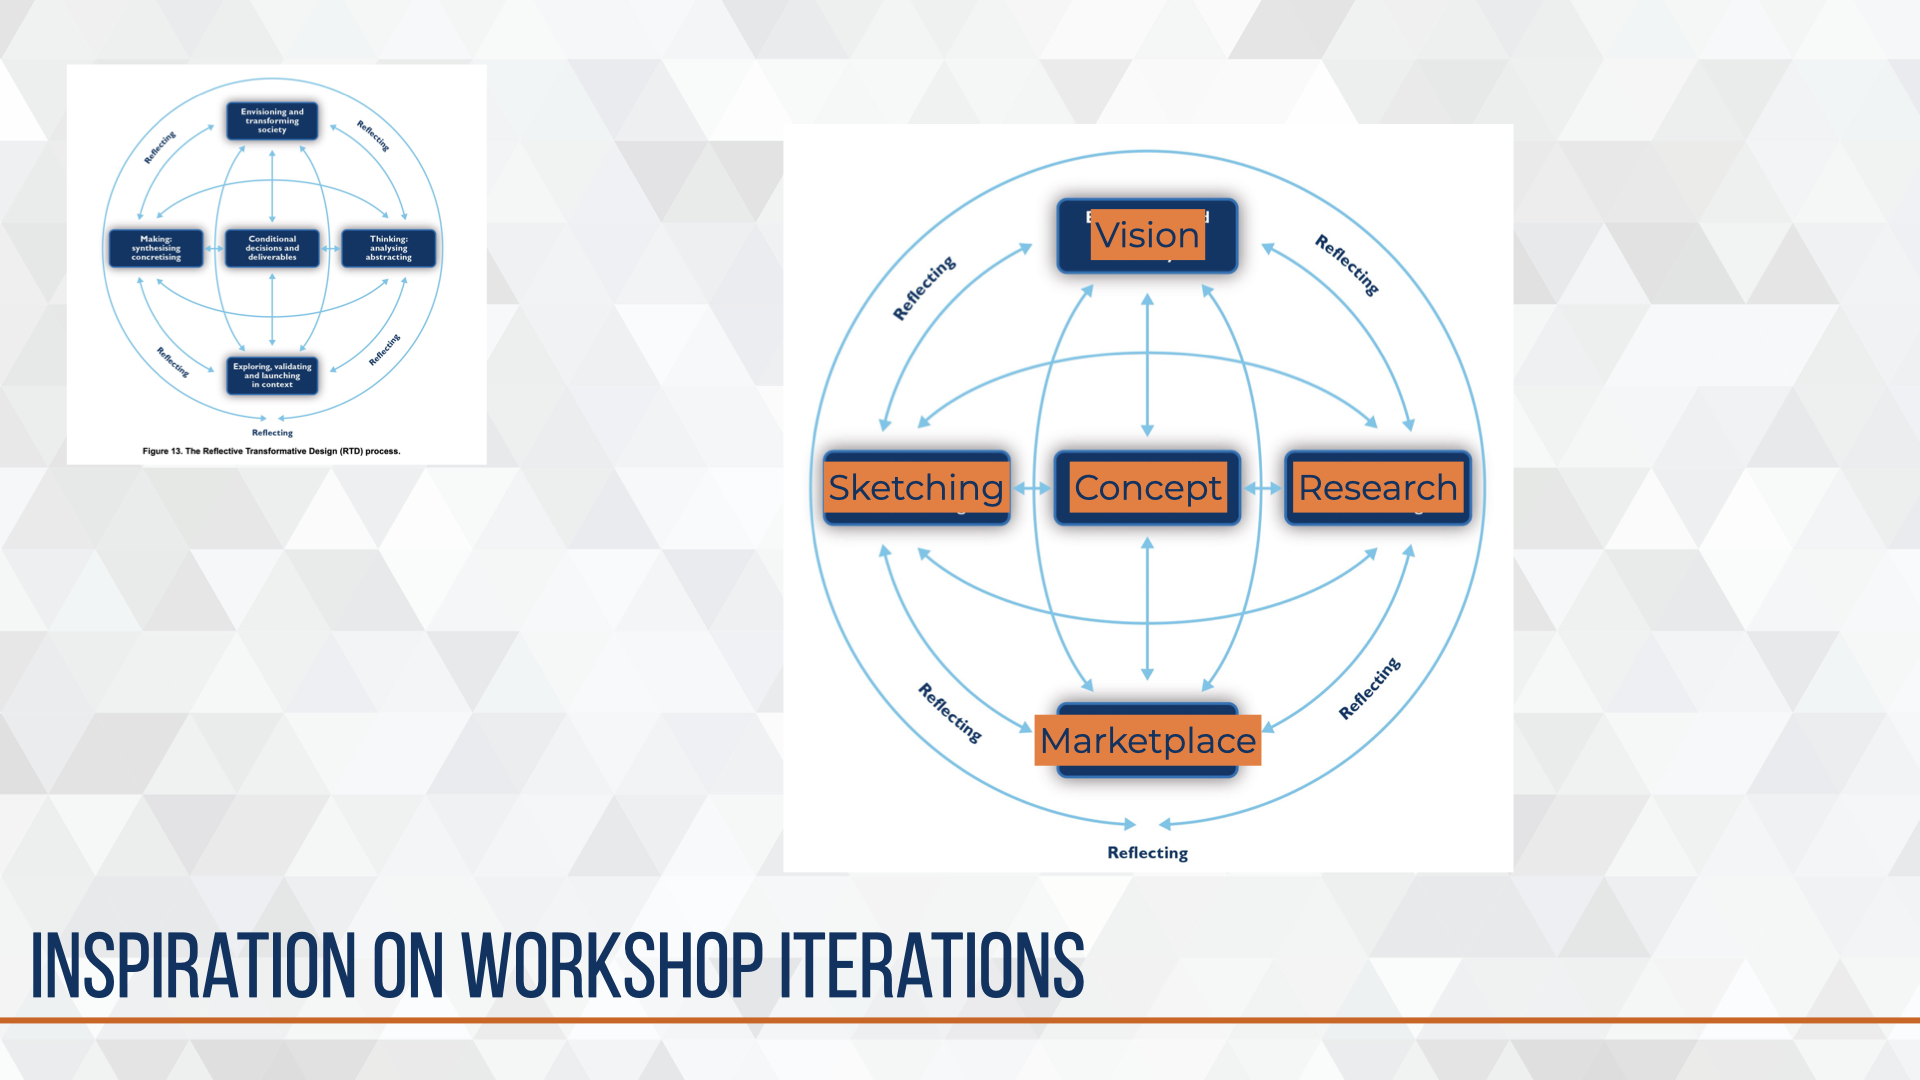
\includegraphics[width=26.67in]{data/keynote-slides/20200430-CDE-Designprocess/20200430-CDE-Designprocess.024-1} \caption{Het RTDP-process is gebruikt als inspratie en methode om het MD\&I te ontwikkelen.}\label{fig:unnamed-chunk-32}
\end{figure}

\textbf{laatste ontwerp canvassen}

\begin{figure}
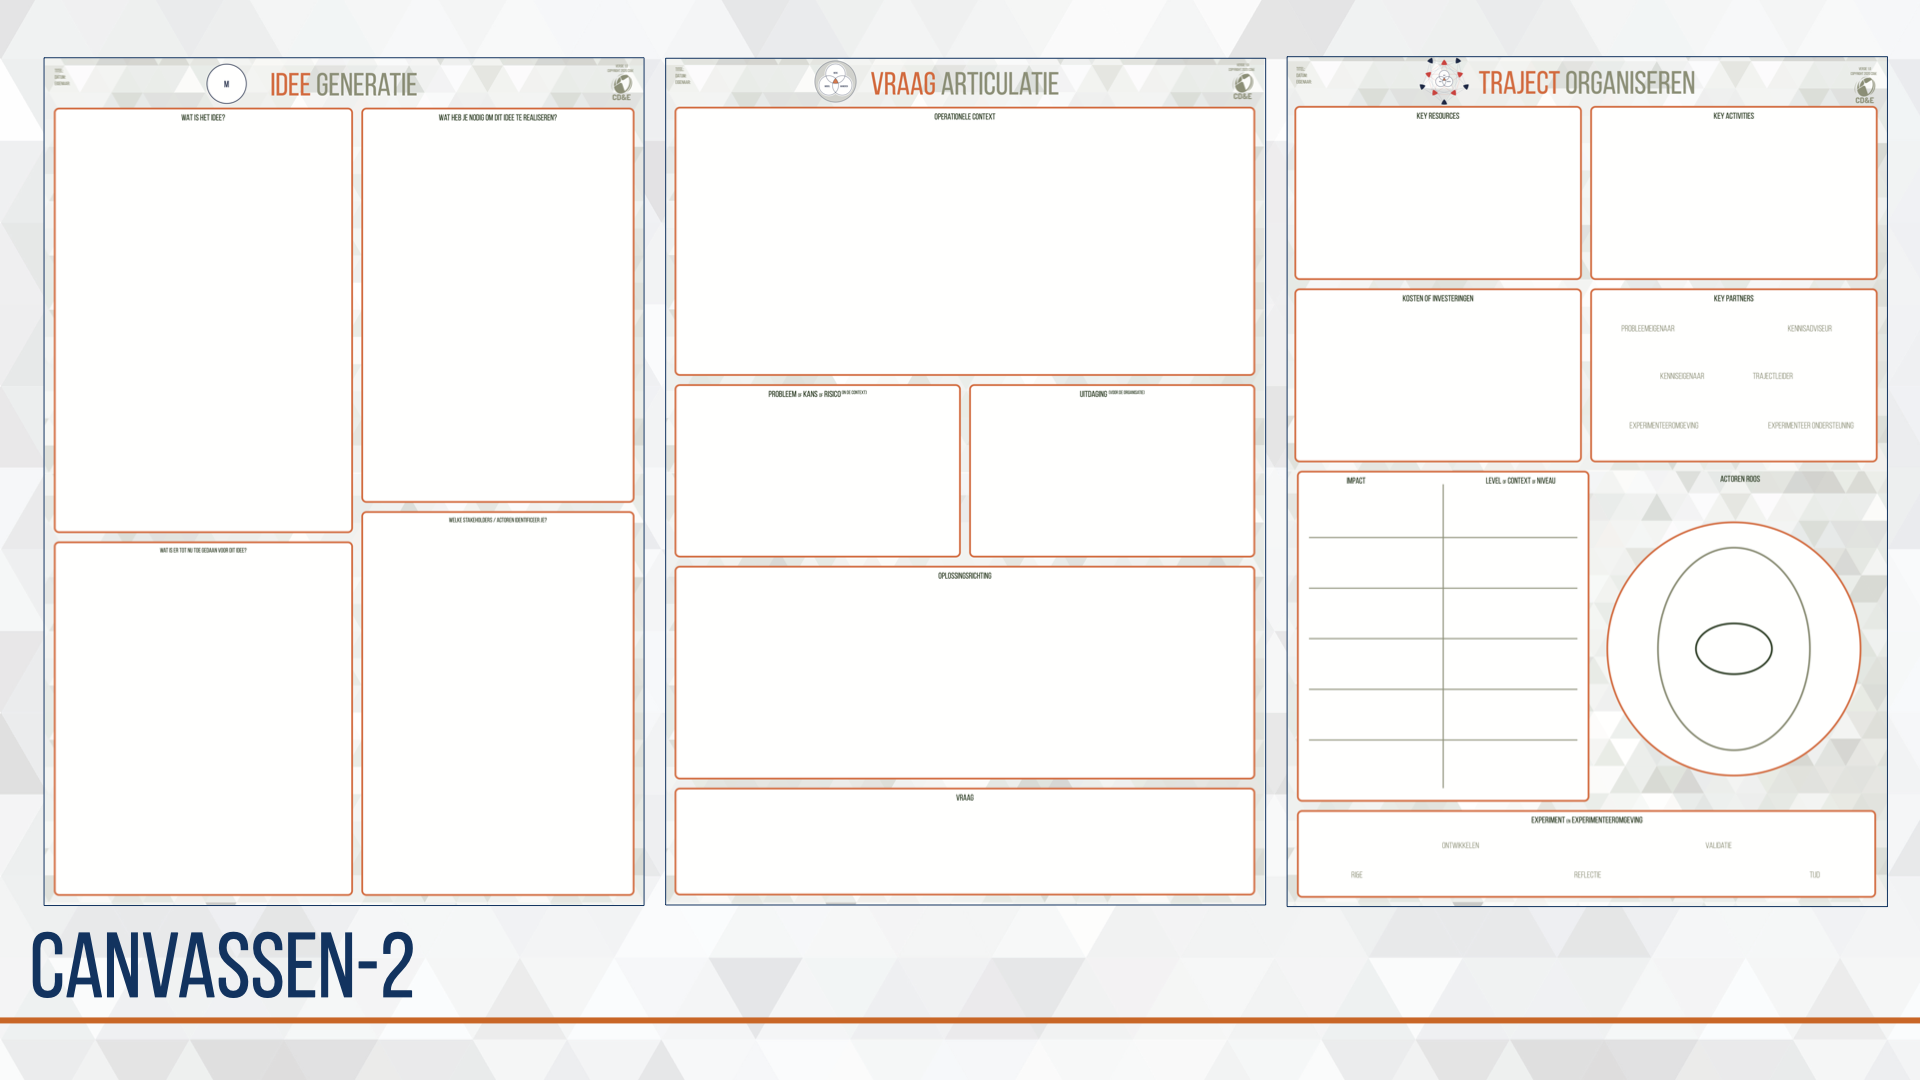
\includegraphics[width=26.67in]{data/keynote-slides/20200430-CDE-Designprocess/20200430-CDE-Designprocess.025} \caption{Final ontwerp canvassen.}\label{fig:unnamed-chunk-33}
\end{figure}

\hypertarget{design-keten-proces-2019-2020}{%
\section{design-keten-proces 2019-2020}\label{design-keten-proces-2019-2020}}

\begin{figure}
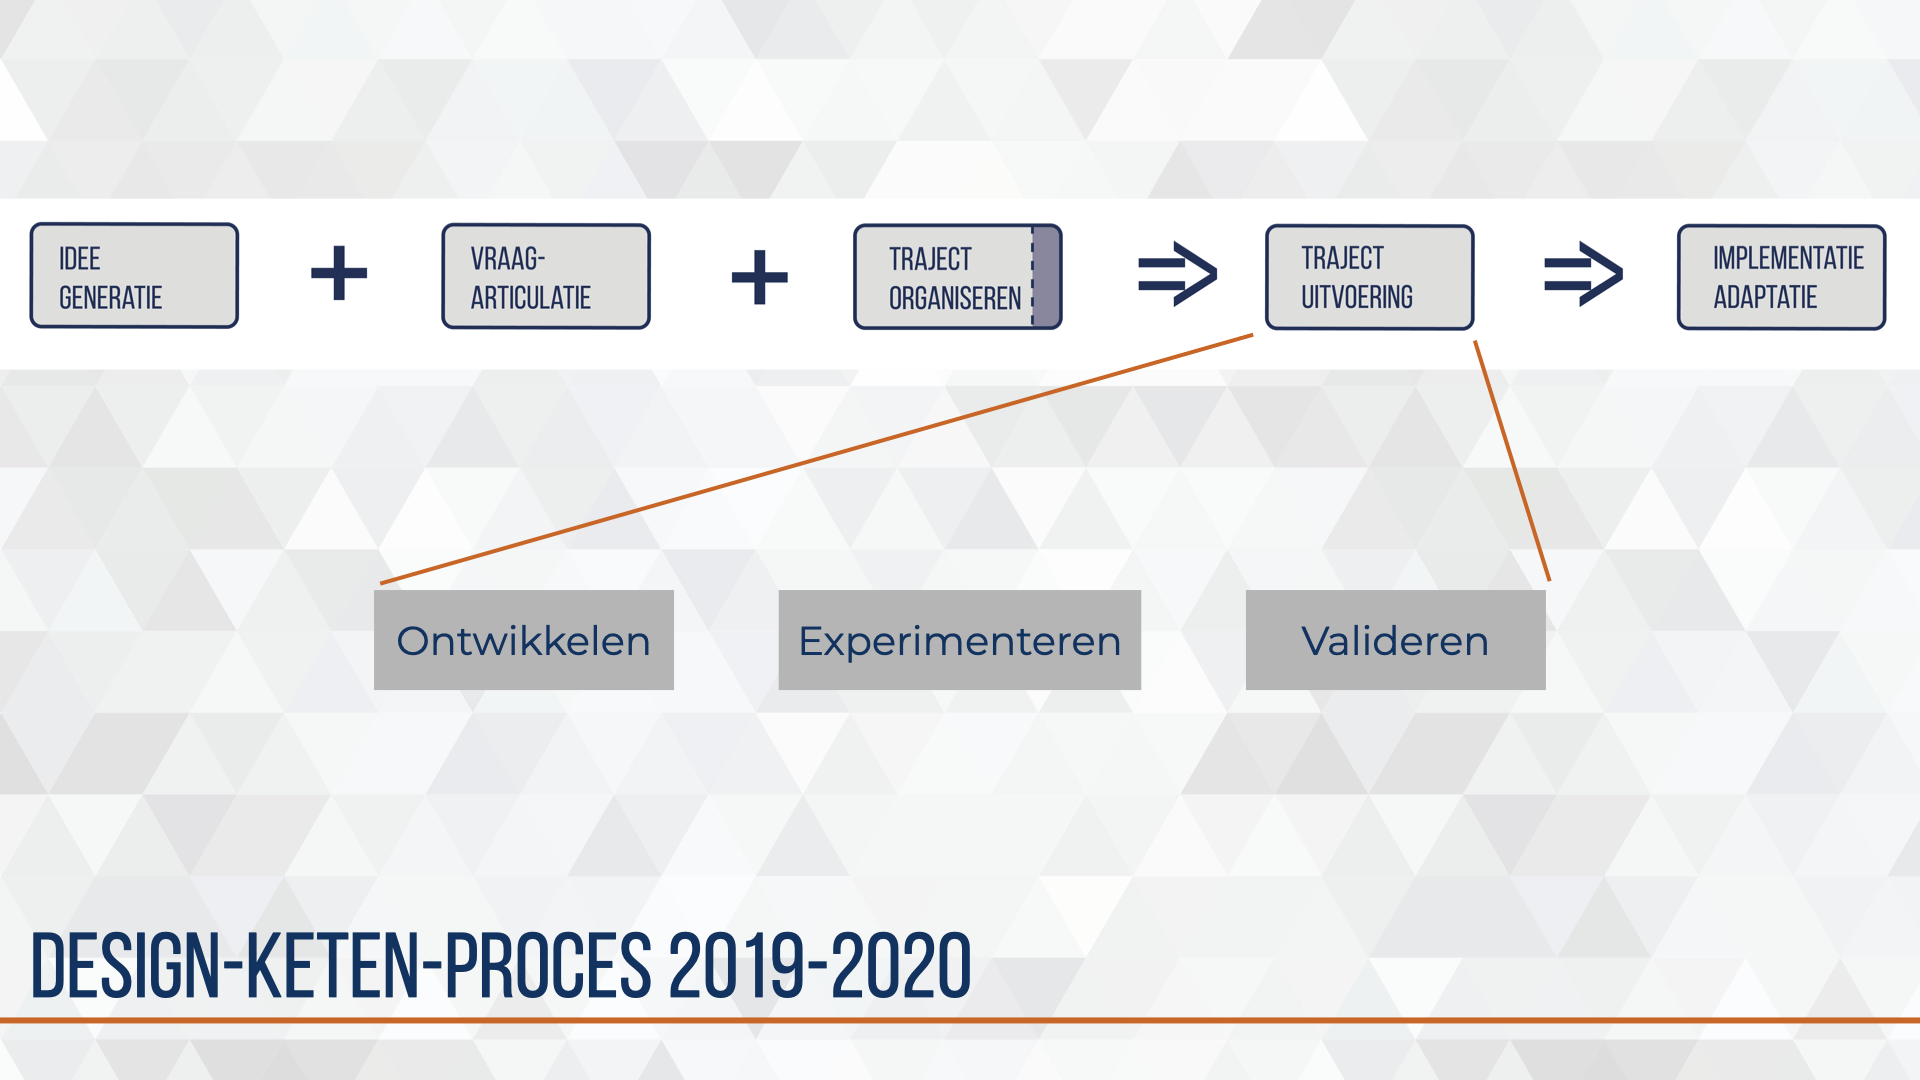
\includegraphics[width=26.67in]{data/keynote-slides/20200430-CDE-Designprocess/20200430-CDE-Designprocess.026} \caption{Verdieping van de uitvoering in drie activiteiten in 2019. }\label{fig:unnamed-chunk-34}
\end{figure}

Bij het toenemen van vraag naar CD\&E faciliteiten en -steun groeide het aantal trajecten. Hierdoor konden de CD\&E-medewerkers reflection in action toepassen op de wijze waarop hun werk wordt verricht. Hieruit komen het CD\&E design keten proces, de rol van Trajectbegeleiders en de ontwikkeling van instrumentarium om het werk en het proces te ondersteunen. Deze werden getest en verder verdiept door het opleiden en begeleiden van nieuwe CD\&E-medewerkers die gedurende twee jaar het team kwamen versterken.

Het woord traject is geïntroduceerd om het discours en de mindset te richten op het onderscheidende van deze aanpak ten opzichte van een standaard landmacht project aanpak. Het traject start met een idee en eindigt bij succesvol doorlopen tot formele opname in de organisatie.

Ieder traject van idee naar implementatie is uniek en bestaat uit een keten van bouwstenen specifiek voor het voorliggend vraagstuk.

\begin{figure}
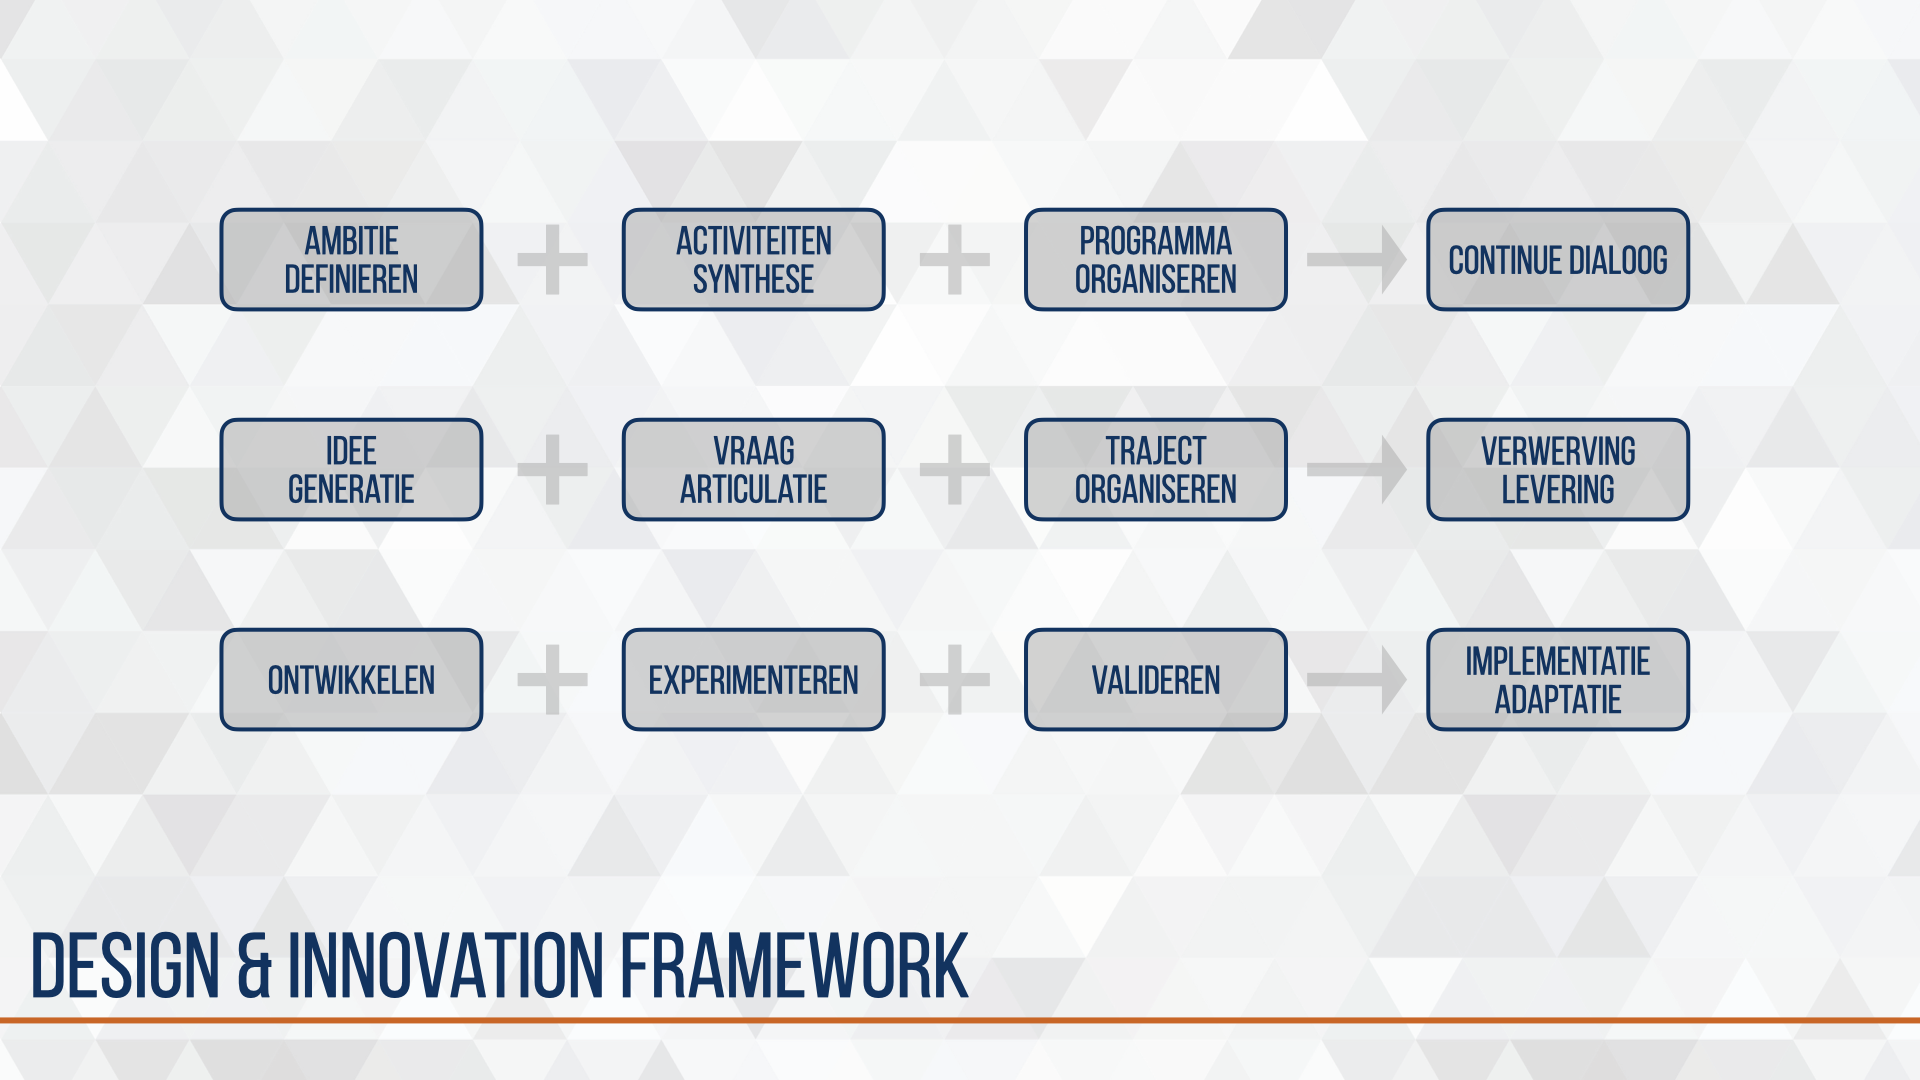
\includegraphics[width=26.67in]{data/keynote-slides/20200430-CDE-Designprocess/20200430-CDE-Designprocess.027} \caption{ }\label{fig:unnamed-chunk-35}
\end{figure}

\hypertarget{refs}{}
\begin{CSLReferences}{1}{0}
\leavevmode\vadjust pre{\hypertarget{ref-awti-2014}{}}%
Adviesraad voor het Wetenschaps- en Technologiebeleid. (2014). \emph{De kracht van sociale innovatie}.

\leavevmode\vadjust pre{\hypertarget{ref-context}{}}%
Context. (n.d.). In \emph{Oxford Online Dictionary}. \url{https://www.lexico.com/definition/context}

\leavevmode\vadjust pre{\hypertarget{ref-gardien_changing_2014}{}}%
Gardien, P., Djajadiningrat, T., Hummels, C., \& Brombacher, A. (2014). \emph{Changing your {Hammer}: {The} {Implications} of {Paradigmatic} {Innovation} for {Design} {Practice}}. \emph{8}(2), 22.

\leavevmode\vadjust pre{\hypertarget{ref-klinkers_navigeren_2014}{}}%
Klinkers, L., Bosboom, F., Königs, M., \& Robertus, H. (2014). Navigeren op waarden: Nieuw gereedschap voor complexe opgaven. \emph{Bestuurswetenschappen}, \emph{68}(2), 92--106. \url{https://doi.org/10.5553/Bw/016571942014068002008}

\end{CSLReferences}

\end{document}
